\documentclass[brazil,ruledheader]{abnt}
\usepackage[T1]{fontenc}
\usepackage[utf8]{inputenc}
\usepackage[brazilian]{babel}
\usepackage[num]{abntcite}
\usepackage{graphicx}
\usepackage{picinpar}
\usepackage{multicol}
\usepackage[small,bf]{caption}
\usepackage{amsthm}
\usepackage{epigraph}

\makeindex

\newtheorem{teorema}{Teorema}[chapter]
\newcommand{\conferir}{\textbf{(conferir)}}

%%Citações entre colchetes
\renewcommand{\cite}[1]{[\citeonline{#1}]}
\makeatletter
\ifthenelse{\boolean{ABCIbiblabelonmargin}}
{
  \renewcommand{\@biblabel}[1]%
  {\ifthenelse{\equal{#1}{}}{}{{\citenumstyle [#1]\hspace{\biblabelsep}}}}
}
{
  \renewcommand{\@biblabel}[1]%
  {%
    \ifthenelse{\equal{#1}{}}
    {}
    {%
      \def\biblabeltext{{\citenumstyle [#1]\hspace{\biblabelsep}}}%
      \settowidth{\ABCIauxlen}{\biblabeltext}%
      \ifthenelse{\lengthtest{\ABCIauxlen<\minimumbiblabelwidth}}
      {\setlength{\ABCIauxlen}{\minimumbiblabelwidth-\ABCIauxlen}}
      {\setlength{\ABCIauxlen}{0cm}}%
      {\biblabeltext\hspace{\ABCIauxlen}}%
    }%
  }%
}
\makeatother

\begin{document}

\autor{Bruna Amin Gonçalves}

\titulo{Análise do Comportamento dos Investidores na Complexidade do Mercado de
Ações}

\orientador{Prof. Allbens Atman Picardi Faria}

\instituicao{Centro Federal de Educação Tecnológica de Minas Gerais}

\local{Belo Horizonte - MG, Brasil}

\data{julho de 2011}

\capa

\folhaderosto

\newpage
\begin{center}
{\huge \emph{\textbf{Dedicatória}}} \\
\end{center}

\vfill
\hspace{.45\textwidth} % posicionando a minipage
\begin{minipage}{.5\textwidth}
\begin{espacosimples}
Aqui vem a dedicatória
\end{espacosimples}
\end{minipage}
\vfill


\newpage
\begin{center}
{\huge \emph{\textbf{Agradecimentos}}} \\
\end{center}

Aqui vão os agradecimentos.

\newpage

\vspace*{\fill}

\epigraph{Aqui vai a epígrafe}{Aqui vai o autor}

\vspace*{\fill}

\tableofcontents

\listoffigures

\begin{resumo}
 resumo
\end{resumo}

\begin{abstract}
 abstract
\end{abstract}


\chapter{Introdução}



As análises e modelagem do mercado financeiro começaram em 1900 com o trabalho
pioneiro do matemático francês Bachelier \cite{MaPaSt99}. Em 1940, Majorana
começou a se interessar por sistemas financeiros e econômicos, sendo o primeiro
a escrever um artigo sobre a analogia entre a física estatística e as ciências
sociais \cite{ChToPaAb10}. A partir de 1950, essas análises do mercado
financeiro se tornaram uma área de pesquisa de grande importância da matemática
financeira e econômica, com vários trabalhos propostos \cite{MaPaSt99}.
Em 1997, Benoit Mandelbrot lançou o livro ``Fractals and Scaling in Finance''
\cite{Ma97}, no qual estuda as flutuações da Bolsa segundo suas próprias
teorias. Propõe que o gráfico anual da Bolsa é semelhante ao mensal e este ao
diário. Essa propriedade, típica dos fractais, é chamada de
auto-autossimilaridade. Assim, foi somente a partir de 1990, que vários físicos
começaram a se interessar por esse assunto interdisciplinar \cite{ChToPaAb10},
demonstrando interesse explícito sobre a investigação na economia. Utilizando
ferramentas e paradigmas de sua própria disciplina, eles criaram uma nova área,
a ``Econofísica`` (com a cooperação de matemáticos e economistas). A palavra
``econofísica'' refere-se a uma fusão das palavras economia e física.

A econofísica aplica ideias, métodos e modelos da física estatística e de
sistemas complexos para analisar e quantificar dados advindos de fenômenos
econômicos. Seu objetivo é entender o comportamento dos agentes e das
instituições econômicas, como consumidores, firmas, mercados de ações e câmbio
para, eventualmente, fazer previsões. Alguns de seus principais focos são os
preços dos ativos (ações, taxas de câmbio e mercadoria) e a distribuição de
riqueza. Pode-se dizer que tudo o que é abordado nos estudos de economia também
pode ser estudado pela econofísica. Um assunto de extrema importância em
economia são as bolsas de valores, pois permitem uma canalização rápida das
poupanças para transformação em investimentos, possibilitando às empresas que
vendem suas ações utilizar esses investimentos na criação de novos
empreendimentos e trazendo, como consequência, novos postos de trabalho, maior
consumo, mais dinheiro em circulação. Em síntese, provocam o aquecimento da
economia. 
Devido à sua importância e contínua expansão, o mercado financeiro requer grande
investimento em recursos humanos para se quantificar e minimizar os riscos das
instituições financeiras envolvidas.

Fatores psicológicos podem causar impactos e crises nos mercados financeiros.
Logo, a investigação para se compreender o comportamento de investidores no
mercado de ações, atualmente, tem-se tornado foco de pesquisas de estudiosos em
economia \cite{ChToPaAb10,So02,WeYiFaWa03,BaHaKhRa10,FaYiWaWe09}. Tal
motivação está relacionada também a fatos históricos de grandes quedas de
mercados, que causaram grandes catástrofes financeiras em algumas partes do
mundo. Antes de cada colapso, os economistas dizem que a economia está no melhor
dos mundos. Bolsas sobem mais e mais. Isso explica por que uma crise pega a
maioria das pessoas, especialmente os economistas, totalmente de surpresa. Duas
importantes teorias da economia tentam investigar esses fatores psicológicos. 

Segundo a economia neoclássica \cite{So02}, os investidores são racionais e
incorporam imediatamente as novas informações do mercado, processando-as para
encontrarem os preços justos e, assim, tornar o mercado eficiente. Mas um novo
campo, chamado de finanças comportamentais, incorpora conceitos da psicologia,
sociologia e outras ciências, visando à aproximação da teoria de finanças a
realidade dos mercados financeiros. Pesquisas empíricas vêm mostrando que o
comportamento dos investidores muitas vezes foge à racionalidade. No
comportamento racional, não caberiam traços psicológicos como excesso de
confiança, indecisão, exagero e, portanto, não abriria a possibilidade para a
ocorrência de crises.

O mercado de ações pode ser comparado a um ecossistema complexo, pois
trata-se de um sistema dinâmico em que cada indivíduo (investidor) busca
assegurar a própria sobrevivência (investimento). Modelos que avaliam o
comportamento de multidões têm sido desenvolvidos para se compreender melhor a
dinâmica dos agentes no mercado financeiro.

Nos modelos econômicos atuais, o agente representativo é
perfeitamente racio\-nal e tem como objetivo maximizar suas ações. Modelos
baseados em agentes, com origem na física estatística, conseguem ir além das
teorias do protótipo dos ``agentes'' da economia tradicional.

Recentemente \cite{WeYiFaWa03,BaHaKhRa10,FaYiWaWe09}, foi proposto um modelo de
autômato celular, uma técnica comum em física estatística, para simular um
mercado de ações artificial e estudar como a psicologia dos investidores
interfere no mercado de ações, considerando dois tipos de comportamento: 
imitadores, que são influenciados pela
preferência da maioria de seus vizinhos, e os anti-imitadores, que adotam a
posição contrária da maioria dos vizinhos. Para validar os modelos propostos,
foram utilizadas técnicas oriundas da física estatística \cite{MaSt00}, como
o cálculo do expoente de Hurst, para analisar as séries temporais da dinâmica da
escolha de investimento em \cite{FaYiWaWe09}.

Neste trabalho, foi criado um mercado artificial, utilizando duas abordagens: a 
primeira os autômatos celulares (CA), para estudar o comportamento do
mercado em função da preferência dos investidores. A segunda abordagem
foi baseada
em redes complexas, para levar em conta, também, o fato de que os investidores
se relacionam por meio de redes sociais e que esses contatos podem influenciar
sua decisão. Além dos dois tipos de investidores acima, criamos mais dois tipos,
os indiferentes, aqueles que tomam suas decisões independentemente do estado da
vizinhança e o “imitador do mais rico”, aquele que imita o investidor que lucra
mais em certo estado de tempo, entre seus vizinhos.  Utilizaremos os
fractais, \emph{random walk} e as técnicas da mecânica estatística (como o
expoente de Hurst) para analisar as séries temporais do índice das ações
produzido pelo modelo e comparar os resultados com mercados reais \cite{CaTa08,
CaTa04}, a fim de verificar se os resultados possuem grau de
complexidade estatisticamente coerentes com mercados reais. 

Este projeto está dividido da seguinte forma: no capítulo
\ref{topicos-em-economia}, é feita uma breve revisão da literatura a respeito de
algumas das principais teorias da economia que analisam o comportamento do
investidor; no capítulo \ref{Métodos-de-Análise}, são apresentados os números
aleátorios, os autômatos celulares e redes complexas que são usados na
construção do modelo; no mesmo capítulo, temos o \emph{random walk}, geometria
fractal e o expoente de Hurst  que são técnicas usadas para analisar e comparar
os
resultados do mercado artificial como os mercados reais; no capítulo
\ref{modelo}, é feita a descrição do modelo; Já no capítulo \ref{resultados},
apresentam-se os resultados; finalmente no capítulo
\ref{conclusao-perspectivas}, são apresentadas as conclusões e perspectivas.   


\chapter{Tópicos em Economia}\label{topicos-em-economia}

Um dos temas mais importantes na teoria de finanças é a hipótese do mercado
eficiente (HME). No entanto, nos últimos anos esse tema passou a ser
questionado por
estudos que demonstraram evidências sobre a existência de um comportamento
anormal nos retornos de ativos financeiros (``anomalias''), devido a
aspectos comportamentais dos agentes econômicos. Ainda é incipiente o
debate sobre este assunto, com defensores da hipótese do
mercado eficiente de um lado, e do outro os adeptos da abordagem baseada em
finanças
comportamentais.
Nesta seção, serão  abordados aspectos relacionados à 
Economia que são extremamente importantes para o desenvolvimento e
entendimento deste trabalho.

\section{Arbitragem}

Geralmente, os preços dos ativos obedecem à lei do preço único, segundo a qual
em mercados competitivos os preços dos ativos equivalentes devem ser os
mesmos. Também é esperado que o preço do ativo deva ser o mesmo em todo
mundo, considerando-se que este se expressa na mesma moeda e que os custos de 
transações possam ser negligenciados. A violação da lei do preço único leva
à arbitragem, que é a compra e venda de um mesmo artigo com o fim de lucrar
com discrepâncias de preços.

Pode-se ilustrar essa concepção, através de dois
exemplos \cite{MaSt00}:

\begin{citacao}
Um quilo de laranja custa 0,60 euros em Nápoles e 0,50 USD em Miami; o
custo de armazenamento e transporte de 1 kg dessa laranja de Miami para
Nápoles é de 10 euros. Comprando 100.000 kg de laranja em Miami e
vendendo em Nápoles, é possível obter um lucro de 10.000 euros.


Um estoque é negociado em dois mercados de bolsas de valores, em cidades
com diferentes moedas, Milão e Nova York. O preço da moeda de ações é 9
USD em Nova York e 8 euros em Milão e a taxa de câmbio entre as duas
moedas é 0,80. Foram compradas 1000 ações em Nova York e vendidas em
Milão, obtendo-se, assim, um lucro (além de custos de transação) de 1000
USD.
\end{citacao}

No exemplo da laranja, se essa ação for realizada várias vezes
sistematicamente, a demanda de laranja aumentará em Miami e diminuirá em
Nápoles. Depois de um tempo, os preços, em ambas localizações, tornar-se-iam
mais racionais (preços competitivos) e, assim, não poderão fornecer oportunidade
de arbitragem. Já o segundo caso ilustra um exemplo sobre os negociadores
do mercado de câmbio, que geralmente ganham a vida tentando encontrar
oportunidades do maior lucro.

A procura de comerciantes por condições de arbitragem contribui para uma
evolução mais racional dos preços nos mercados e, consequentemente, para
a descoberta de novas oportunidades de arbitragem. Se um comerciante obtiver
lucro  na venda de certo artigo, ele provavelmente repetirá a mesma ação.

\section{Hipótese de Mercado Eficiente (HME)}

O conceito de mercado eficiente é estreitamente relacionado à ausência
de arbitragem, ou seja, é tido como um mercado ideal, sem arbitragem, mas
sua definição não se resume somente a isso. Segundo definição de acadêmicos
em finanças, o mercado altamente eficiente é determinado pelo maior número
de preços racionais de ativos negociados. As alterações dos preços de ações
podem ser devidas a diversos fatores como relatório de ganhos, 
prognóstico de desempenho da empresa, uma nova perspectiva para a evolução
da indústria, eventos políticos, ou até mesmo boatos sobre a gestão da
empresa\cite{Sc05,MaSt00}. 

A hipótese de mercado eficiente (HME) foi formulada no início do século XX
com o trabalho pioneiro de Bachelier, que propôs que os preços dos ativos
no mercado especulativo poderiam ser descritos por um processo estocástico.
Desde 1960 várias investigações empíricas têm sido devotadas para provar
a hipótese do mercado eficiente. A definição formal da HME foi feita por
Fama apenas em 1965 \cite{Sc05}. E, no final de 1980, após uma análise rigorosa,
Lo e MacKinlay, concluíram que, se os preços seguem um \emph{random walk}
(passeio aleatório), isso é condição suficiente para a HME \cite{MaSt00}.

Duas hipóteses são importantes para a HME: a primeira diz que os preços
do mercado seguirão um \emph{random walk} se suas variações forem aleatórias
e independentes; já a segunda hipótese é a de que os investidores são racionais,
ou seja, imediatamente incorporam as novas informações do mercado,
utilizando-as para atualizar, em seguida, os preços dos ativos.

Três formas de HME são propostas e discutidas na literatura
econômica moderna:

A primeira, chamada forma fraca, diz que os preços atuais refletem
toda informação referente aos preços antigos, ou seja, os retornos
passados predizem retornos futuros. Sob tal ponto de vista, nenhum
investidor poderia obter retornos em excesso, mediante a análise de
preços passados. Assim, informações contidas nos preços passados não
seriam relevantes para obter um retorno em excesso.

Na segunda forma, que é chamada semi-forte, investiga-se se todas as
informações públicas são refletidas no nível atual. Ou seja, preços não
refletem apenas as informações passadas, mas também as informações públicas
como notícias e anúncios. Logo, nenhum investidor poderia obter retorno
em excesso fazendo operações baseadas nas análises de relatórios anuais
de empresas, notícias públicas ou outras fontes de informação publicadas.

Já na terceira forma, chamada forma forte, consideram-se todos os fundamentos
do mercado (informações públicas e não-públicas) na análise, ou seja, todas
as informações que podem ser obtidas, inclusive as chamadas
informações privilegiadas. A forma forte da HME não encontra muitos
defensores entre os economistas, de modo que os debates sobre HME se
limitam, geralmente, às formas fraca e semi-forte.

Em 1980, com a intensificação da pesquisa nessa área, foi evidenciada
a existência de comportamentos anormais nos retornos dos ativos
financeiros. Dessa forma, esta teoria passou a ser questionada no meio
acadêmico. As observações empíricas mostram que é difícil prever mudanças
de preços, mas não impossível, contestando, assim, a hipótese de
mercado eficiente.

A teoria da complexidade algorítmica \cite{MaSt00}, definida sobre o
conjunto de strings binários, foi desenvolvida por Kolmogorov e Chaitin, em
meados de 1960. Para  ilustrar esta concepção, suponha que se queira transportar
informações sobre realizações científicas e sociais de raças humanas para
regiões fora do sistema solar. Entre as informações, será colocado o valor de
pi com 125.000 pontos e o valor das séries temporais de valores diários
do Dow-Jones com 125.000 dígitos. Para minimizar o armazenamento e transmissão
de tempo é necessário usar duas sequências numéricas em algoritmos
específicos. No armazenamento dos dígitos do pi foi encontrado um algoritmo
de custo barato, cujo valor é extremamente pequeno. Em contraposição,
um algoritmo com eficiência comparável não foi encontrado para o
índice Dow-Jones.

O resultado dessa experiência explica-se pelo fato de que uma série de
símbolos dentro da teoria da complexidade algorítmica é considerada
imprevisível se as informações não puderem ser comprimidas. As séries
temporais de mudança de preço no mercado financeiro carregam uma
grande quantidade de informação não redundante, o que dificulta a extração de
um sub-conjunto de informações econômicas associadas a alguns
aspectos específicos. Se uma determinada informação afeta o preço, o mercado
não é completamente eficiente.

Essa teoria ajuda compreender o comportamento de uma série temporal
financeira, pois retrata a clara conexão entre a hipótese de mercado eficiente
e a imprevisibilidade de ações de retorno.

A racionalidade também passou a ser questionada por Keynes, para quem um
``espírito animal'' governa o comportamento dos investidores, ou seja, eles
não podem ser completamente racionais. Ações de diferentes
investidores, aparentemente racionais, podem variar significativamente levando
a diferentes percepções de mercado e eventos \cite{Sc05}. Além disso, os
investidores poderão ter diferentes recursos para a aquisição e processamento
de novas informações. No próximo capítulo será apresentada a teoria de
finanças comportamentais.

\section{Finanças Comportamentais}

Teorias sobre o comportamento humano importadas da psicologia e da sociologia
têm ajudado a dar maior sustentação teórica aos estudos empíricos sobre
a dinâmica dos mercados financeiros. Assim, auxiliando-se da incorporação
de conceitos dessas áreas à economia, busca-se compreender as
decisões financeiras dos indivíduos através da análise da hipótese de que
os mercados refletem os pensamentos, emoções e ações de pessoas reais.

Na teoria tradicional, aspectos psicológicos do investidor são ignorados. O
mundo é
composto por agentes que pressupõem que os preços nos mercados
financeiros incorporam todas as informações disponíveis; sendo assim, o preço do
ativo representa a melhor
estimativa do  valor dos ativos que estão sendo negociados. Estudos empíricos
têm mostrado que existem inúmeras situações em que os agentes não se
comportam segundo a racionalidade prevista pela HME. Geralmente, um
investidor racional tenta otimizar suas ações, mesmo que a racionalidade tenda
a ser dificultada por vieses cognitivos, emocionais e influências sociais.

O principal objetivo dos acadêmicos que atuam no campo  das
finanças comportamentais é mostrar que existem limites à racionalidade
que ocorrem com frequência signi\-ficativa para provocar implicações
econômicas relevantes. Visam, ademais,  incorporar tais limitações ao estudo
da teoria econômica a fim de promover maior entendimento dos fenômenos
econômicos no campo teórico.

Thaler, da Universidade de Chicago, foi um dos primeiros e mais fortes
defensores da economia comportamental \cite{So02}. Através de seus estudos,
ele questiona a economia neoclássica onde os mercados são eficientes e as
pessoas são racionais. Thaler observou e relatou o comportamento de alguns
colegas supostamente racionais: No primeiro exemplo, ele cita o caso de um
amigo que, para economizar \$ 10 corta seu próprio gramado, mas admitiu que
nunca concordaria em cortar o gramado vizinho em troca dos mesmos \$ 10 ou
até mais. De acordo com o conceito de custo de oportunidade, um ganho de \$
10 para cortar um gramado vizinho é a mesma coisa que pagar alguém para cortar
o seu próprio gramado. O segundo exemplo é de um amigo que deixou de ir a um
jogo de basquete por causa de uma tempestade de neve. Tal amigo comentou que
se tivesse comprado os bilhetes, ele teria ido. Esse problema se refere a
custos irrecuperáveis; afinal, o dinheiro já estaria pago. Já em um
terceiro exemplo, uma garrafa de vinho que custa \$ 50 pode parecer muito cara
para  comprar em um jantar informal em casa. Mas se a pessoa já possuir
tal garrafa, provavelmente a usará em tal refeição. Resumindo, pessoas não
se comportam como a economia racional prevê.

Uma anomalia chamada de ``desconto hiperbólico'' \cite{So02} refere-se à
inversão
de preferência: quando as pessoas estão para receber certo dinheiro, elas são
capazes de planejar, muito racio\-nalmente, quanto gastar imediatamente e
quanto guardar. Isso está de acordo com a teoria econômica, que argumenta
que pessoas estão dispostas a poupar e adiar gastos. Mas, quando o
dinheiro realmente chega, muitas vezes é gasto imediatamente. Em outras
palavras, quando os sacrifícios estão em fase de planejamento, a
racionalidade predomina. Tais preferências, negligenciadas pela
economia neoclássica, têm implicações importantes para poupança dos
investidores.

Essas análises reforçam a idéia de que os consumidores não são
completamente racionais, mas sim influenciados por suas emoções.
Tal comportamento também pode ser observado nos investidores do mercado de
ações.

No mercado de ações o preço de um ativo, em dado instante de tempo, é
determinado a partir do equilíbrio entre oferta e demanda: se houverem
mais pessoas ``comprando'' do que ``vendendo'' ações, os preços serão conduzidos
para cima e vice-versa. Para que haja uma redução (ou aumento) nos preços,
é necessário que os investidores que pretendem comprar (ou vender) estejam
em minoria.

Quando o investidor imita a opção da maioria que está comprando (ou
vendendo) lucrará apenas se o preço subir (ou descer). Quando o investidor
está mantendo, não tem lucro nem prejuízo.

Um fato interessante no mercado de ações é a existência de comportamento
de ``rebanho'', ou ``manada``, dos investidores. Tal característica ocorre
quando muitas pessoas tomam a mesma decisão, devido à tendência a imitar as
ações dos outros. O termo rebanho, obviamente, refere-se ao
comportamento semelhante observado em grupos de animais.

Nos últimos anos, os físicos têm mostrado que grande parte do comportamento
de manada observados em animais pode ser entendida a partir da ação de leis
simples  de interação entre os animais. No que diz respeito aos seres
humanos, sabe-se que quanto menos informação a pessoa tiver, mais forte é
sua tendência a seguir o consenso, ou seja, as pessoas imitam quando
falta informação. Todos os investidores, em quase todo o mundo, estão
organizados em uma rede de família, de amigos, colegas e outros que são as
fontes
de opinião e influenciam uns aos outros localmente através desta
rede. Caracteriza-se como efeito cascata, ou dominó (o mesmo que efeito manada)
quando certo indivíduo
escolhe imitar a ação da multidão ao invés de agir de acordo com suas
informações e se tal decisão for repetida por outras pessoas tornando
esse processo repetitivo.

Às vezes uma estratégia de negociação não é suficiente para saber (ou
adivinhar) a direção do mercado. Existem sutilezas que especificam a forma como
um  investidor vai comprar ou vender uma ação. Por exemplo, um investidor
que quer ficar à frente dos outros investidores, para comprar a ação por um
preço melhor, vai querer sair do mercado antes dos outros, ou seja, antes de
uma inversão da tendência. Dessa maneira, vai ser contrário aos seus
vizinhos (quando a maioria estiver comprando a pessoa vai vender e quando
a maioria estiver vendendo a pessoa vai comprar). Assim, ele estará em minoria
no mercado. Isto leva a uma classe de comportamento contrária à baseada
na imitação, denominada anti-imitação. Podem ocorrer problemas na
utilização desses tipos de informações passadas para tomar a decisão de
comprar, por exemplo, quando a pessoa acredita que os outros investidores
não estarão comprando e se todos também usarem esse mesmo conjunto de
regras, esta pessoa não estará mais em minoria. 

Nos mercados reais, o comportamento dos agentes nem sempre é totalmente
imitador ou anti-imitador. Existem aqueles que têm o seu próprio ponto de
vista, ou seja, investidores que possuem opinião própria (ou
informações privilegiadas). A representação real do mercado exige, portanto, uma
combinação de
todas estas características dos investidores.

\chapter{Métodos de Análise}\label{Métodos-de-Análise}

Nesta seção, serão apresentados  tópicos necessários para análise resultados
como  números aleatórios,  autômatos celulares
e conceitos sobre redes complexas; propriedades da geometria dos fractais, o
\emph{random
walk} e
outras técnicas da mecânica estatística com a finalidade de verificar o grau
de complexidade do mercado de ações proposto.

\section{Números Aleatórios}

Não há como gerar uma sequência realmente aleatória no computador, pois sua
precisão é finita devido ao número limitado de bits.  Assim, alguns critérios
foram estabelecidos para julgar a qualidade dos geradores de números aleatórios:

\begin{itemize}
\item distribuição dos números gerados uniformemente ao longo de um intervalo;
\item números gerados devem ser estatisticamente independentes entre si;
\item o valor de um número, na sequência, não deve afetar o valor do próximo
número;
\item a geração desses números deve ser rápida, de modo a poupar recursos
computacionais para as simulações em si;
\item se forem especificadas as mesmas condições iniciais, a sequência de
números aleatórios gerada deve ser sempre a mesma;
\end{itemize}

O algoritmo deve executar da mesma maneira em diferentes tipos de computadores,
ou seja, a mesma sequência de números aleatórios deve ser gerada em diferentes
tipos de computadores com as mesmas condições iniciais.

Existem diferentes métodos de geração de números aleatórios. Quase todos os
compiladores  incluem, nas suas bibliotecas, geradores de
números
aleatórios. A qualidade desses geradores é variável. Os principais fatores que
devem ser levados em consideração são o custo computacional para gerar uma
sequência e o limite de confiabilidade do gerador. No nosso trabalho optou-se
pelo uso do método linear congruente, que será explicado abaixo.

\subsection{Método Linear Congruente}

O mais conhecido algoritmo para geração de sequências pseudo-aleatórias de
inteiros é o método linear congruente \cite{KlGo06,Fi}:

\begin{equation}
\label{eq:mlc}
 I_{n+1}=(AI_n+C)\bmod{M},n \geq 0
\end{equation}
onde $M$ é o módulo, $0 \leq A<M$ é o multiplicador, $0 \leq C<M$ é o incremento
e $I_0<M$ é a semente. 

No caso em que $C \neq 0$, o gerador congruente é misto, e para $C=0$, o gerador
congruente é multiplicativo. A relação recursiva \ref{eq:mlc} gera o próximo
número inteiro. Para se obter uma variável aleatória uniformemente distribuída,
no intervalo $[0, 1]$, deve-se dividir $I_n$ por $ M:Z_n=\frac{I_n}{M} $.

Esse método pode gerar uma boa sequência de números aleatórios; contudo, se os
valores das constantes não forem selecionados corretamente, depois de algumas
interações, a sequência irá repetir-se sem gerar todos os números possíveis, no
intervalo $[0,M]$.

Se $A$, $C$ e $M$ são corretamente selecionados, a sequência pode chegar a um
comprimento máximo $M$, distribuídos aleatoriamente no intervalo de 0 a $(M-1)$.
O teorema \ref{te:mlc}, a seguir (demonstrado por Hull e Dobell em 1962
\cite{HuDo62}), mostra as condições necessárias para os valores ideais de $A$,
$C$ e $M$.

\begin{teorema}
\label{te:mlc}
 O método linear congruente tem um período $M$ se, e somente se:
\begin{enumerate}
\item[i.] $C$ e $M$ são primos entre si.
\item[ii.] $B=(A-1)$ é múltiplo de $P$, para todo $P$ primo divisor de $M$.
\item[iii.] Se $M$ for múltiplo de 4, então $B$ tem que ser múltiplo de 4.
\end{enumerate}
\end{teorema}

Na linguagem $C$, temos à disposição $2^{31}$ números inteiros, $A =
843314861$ e $C = 453816693$ são números mágicos \cite{St93} que permitem
que o método acima sorteie cada um dos $2^{31}$ números disponíveis
exatamente uma vez antes que a sequência volte a se repetir.

\section{Autômatos Celulares}

Os autômatos celulares (CA's) foram propostos por John Von Neumann e Ulam, na
década
de 60, como uma possível idealização para modelar a auto-reprodução
biológica. São sistemas dinâmicos, discretos, de simples construção, utilizados
como  modelos matemáticos para investigar a auto-organização de sistemas
em diferentes áreas, tais como \cite{Fa02,Bo04,Wo83}: mecânica
estatística, reações químicas, dinâmicas de populações, computação, biologia,
geologia, medicina, até problemas em teoria dos números. São capazes de
descrever sistemas que exibem complexidade mesmo a partir de elementos
simples. De modo geral, consistem de uma rede uniforme (ou vetor) onde o
estado é representado como uma variável discreta em cada sítio (célula). O
estado em um passo de tempo é determinado pelo estado da vizinhança no
passo anterior e as regras de transição podem ser determinísticas
ou probabilísticas \cite{Fa02,Wo83}. 

O interesse no estudo dos (CA's) tem crescido nos últimos anos, fato que
se deve ao sucesso em descrever uma vasta gama de fenômenos nos mais
variados sistemas, pertencentes a diferentes áreas do conhecimento. Todas as
aplicações  hoje existentes foram baseadas nos trabalhos de John Vou
Neumann, John Holton Conway e Stephen Wolfram \cite{CaCa08}. Algumas das
implementações propostas serão abordadas, resumidamente, a seguir.

\subsection{Regras de Evolução (Transição)}

Nos autômatos celulares, $Z^N$ representa a dimensão e $Z_L$ representa
o conjunto de inteiros, no modulo $L$. Se o conjunto de vértices é $Z^N_L$, o
autômato celular possui condições periódicas de contorno.

Para um autômato celular em uma dimensão, as regras são definidas a seguir:
$S^t(i) \in Q$ representa o estado do sítio $i \in Z$ no tempo $t \in N$. A
regra de evolução local é definida pela função: $f: Q^{R_e+R_d+1} \rightarrow
Q$, tal que: 

\begin{equation}
S^{t+1}(i)=f(S^t(i-R_e),S^t(i-R_e+1),\dots,S^t(i+R_d)),
\end{equation}
onde $R_e$ e $R_d$ são, respectivamente, os alcances à esquerda e à direita da
regra $f$. No caso em que $R_e=R_d=R$ é chamado de alcance da vizinhança.

Já em duas dimensões, existem mais possibilidades de vizinhança. $S^t(i,j)$
representa o estado do autômato $(i,j)$ no tempo $t \in N$. O estado
$S^{t+1}(i,j)$, no sitio $(i,j)$, no tempo $t+1$, é determinado pelo estado  dos
vizinhos no tempo $t$, ou seja:

\begin{equation}
 S^{t+1}(i,j)=f\left( \begin{array}{ccc} S^t(i-R_1,j-R_2) & \dots &
S^t(i+R_1,j-R_2) \\ S^t(i-R_1,j-R_2+1) & \dots & S^t(i+R_1,j-R_2+1) \\ \dots &
\dots & \dots \\ S^t(i-R_1,j+R_2) & \dots & S^t(i+R_1,j+R_2) \end{array}\right)
\end{equation}

Onde $f:Q^{(2R_1+1)x(2R_2+1)}\rightarrow Q$ é um autômato celular de duas
dimensões com regra de evolução local.

\subsection{Autômatos Celulares Determinísticos}

Após terem sido propostos por Von Neumann, na década de 1960, os
CA's determinísticos só vieram a ser estudados em detalhes por Stephen Wolfram
em 1983 \cite{Wo83}.

Nos CA’s de Wolfram, o conjunto de vértices é definido em $Z_L$, o estado de
cada
sítio é representado pelos valores binários 0 ou 1  a vizinhança do sitio $i$
no tempo $t$ é composta pelos sítios, $i - 1$ e $i + 1$, ambos no mesmo instante
de tempo.  Assim, a evolução desse autômato depende, deterministicamente, dos
estados de três sítios, ou seja,
$S^{ t+1}(i)=f(S^t(i-1),S^t(i),S^t(i+1))$.\- Dessa forma, existem $2^{2^3}=256$
regras locais diferentes, pois a evolução de cada sítio é determinada por três
sítios tendo duas representações possíveis 0 ou 1; assim o número total de
combinações para uma vizinhança é $2^3$. A regra 50, cujo valor binário é
00110010, está exemplificada na tabela \ref{tab:tab1} e na figura
\ref{fig:arvore}.

\begin{table}[!h]
\centering
\begin{tabular}{|c|c|c|c|c|c|c|c|}
\hline
 000 & 001 & 010 & 011 & 100 & 101 & 110 & 111 \\
\hline
0 & 1 & 0 & 0 & 1 & 1 & 0 & 0 \\
\hline
\end{tabular}
\caption[Regra local possível para um autômato celular.]{Regra local possível
para um autômato celular, na primeira linha é
descrita as oito combinações possíveis para uma vizinhança de três sítios de
estados binários e, na linha de baixo é apresentada a representação binária da
regra 50.}
\label{tab:tab1}
\end{table}
\begin{figure}
\centering
\begin{tabular}{cc}
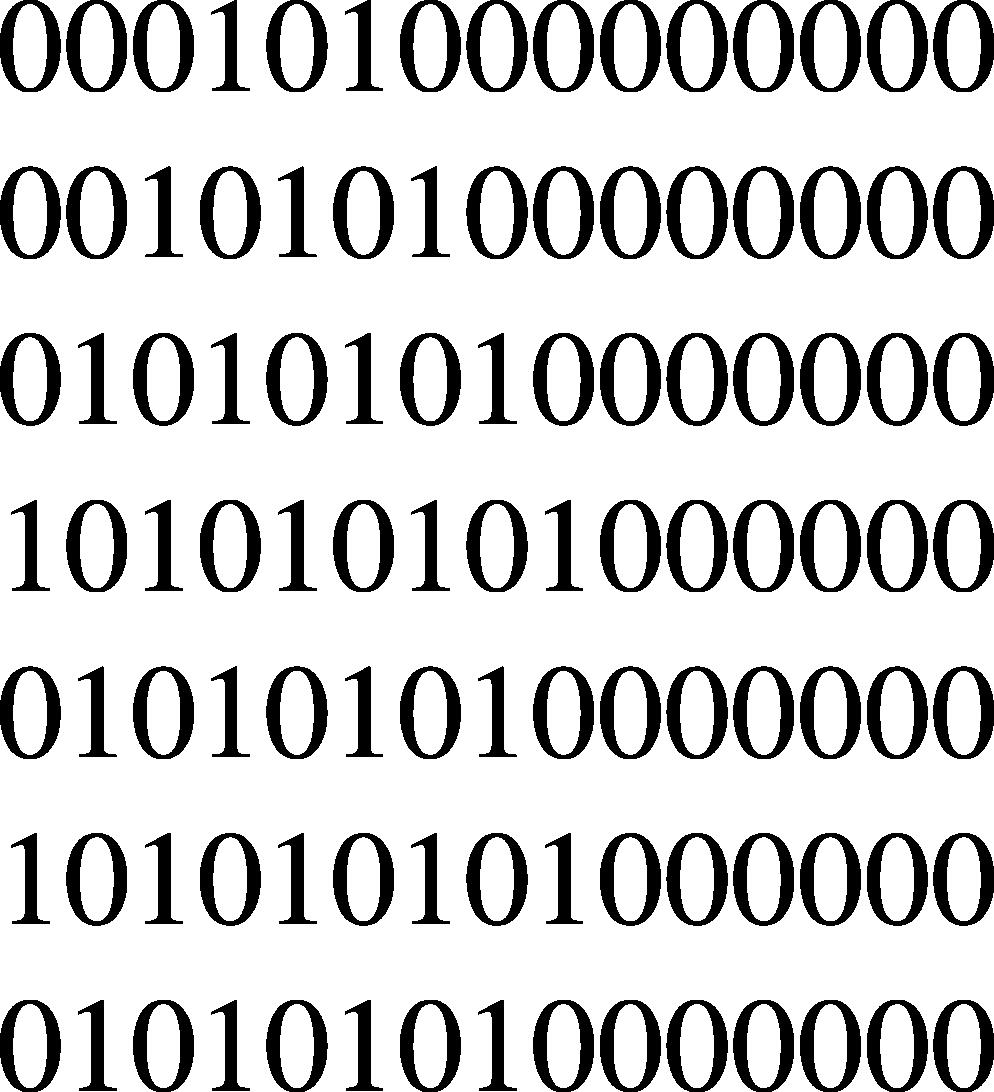
\includegraphics[width=.3\linewidth]{Figuras/figura51.jpg} &
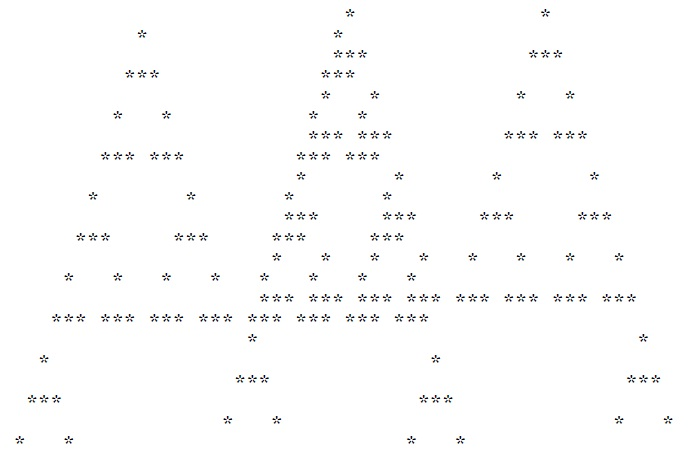
\includegraphics[width=.4\linewidth]{Figuras/figura2.jpg} \\
(a) & (b) \\
\end{tabular}
\caption [Evolução temporal e padrão do autômato]{(a) Evolução temporal do
autômato pela regra 50. A partir das regras
da tabela \ref{tab:tab1}, todos os sítios são atualizados
simultaneamente a cada passo de tempo. (b) Padrão reproduzido pela regra 22. O
estado 1 é representado pelo asterisco e o estado 0 pelo espaço vazio.}
\label{fig:arvore}
\end{figure}


Wolfram verificou todas as regras possíveis, classificando os padrões em
quatro tipos: homogêneo, periódico, caótico e complexo \cite{Wo83}.  Além
disso, sua classificação demonstra que tais regras podem levar a uma espécie
de auto-organização, o que contribui, inicialmente, para uma maior compreensão
do fenômeno de formação espontânea de padrões.

\subsection{Jogo da Vida}

John Holton Conway, em 1970, criou o ``jogo da vida'' \cite{CaCa08,Be}, um
autômato celular que utiliza regras locais para simular alterações em populações
de seres vivos. Nesse modelo, cada célula nasce ou morre de acordo com o estado
das células vizinhas e o jogo apresenta grau elevado de complexidade com
vários cenários possíveis. Os resultados visuais são complexos e
imprevisíveis. Dependendo da situação inicial, mudanças de comportamento
podem surgir.

No jogo da vida, em volta de cada célula são consideradas oito células
vizinhas. O estado de uma célula é representado pelos valores binários 0 ou 1,
que  representam a célula morta e a célula viva, respectivamente. As regras
do jogo são as seguintes:

\begin{enumerate}
\item Qualquer célula, com dois ou quatro vizinhos vivos, continua no mesmo
estado
para a próxima geração.
\item Qualquer célula viva, com menos de dois vizinhos vivos, morre por solidão.
\item Qualquer célula viva, com mais de quatro vizinhos vivos, morre de
superpopulação.
\item Qualquer célula morta, com exatamente três vizinhos vivos, renasce.
\end{enumerate}

\begin{figure}[!h]
 \centering
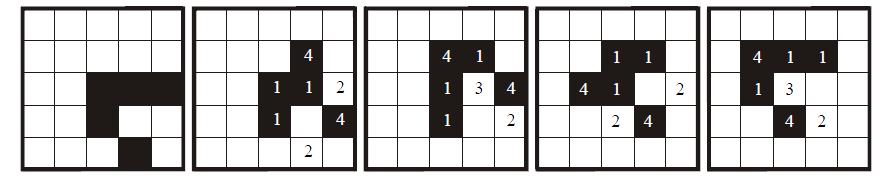
\includegraphics[width= 0.9 \linewidth]{Figuras/figura1.jpg}
\caption [Exemplo de transição do jogo da vida]{Exemplo de transição do jogo da
vida. Os números representam a regra
aplicada no passo anterior e da evolução ao longo do tempo.}
\label{fig:JogoDaVida}
\end{figure}

Os comportamentos semelhantes observados foram classificados em três tipos:
objetos estáveis, onde as configurações iniciais não tendem sofrer modificações
ao longo do tempo; objetos oscilatórios, onde as configurações iniciais, depois
de um determinado período, voltam as suas formas originais. Já o terceiro tipo,
denominado \emph{gliders}, as configurações ciclicamente repetem suas formas,
porém em posições diferentes e se movem através da grade. 



\section{Redes Complexas}

Stanley Milgram, na década de 80, realizou um experimento nos Estados
Unidos, levando em consideração que o número de pessoas conhecidas é
relativamente pequeno em relação à população, e concluiu que duas
pessoas escolhidas aleatoriamente estão ligadas de alguma forma uma à outra
por um caminho de mais ou menos 6 conhecidos, esse fenômeno ficou conhecido
como ``rede de pequeno mundo`` e tem sido verificado em diversas redes sociais
\cite{Bo04,AlBa02}. A propriedade de pequeno mundo
caracteriza a maioria das redes complexas, como por exemplo, os grandes atores
de Hollywood estão na distância média de três atores um do outro e os produtos
químicos 
 são normalmente separados por três reações. Podemos citar como
exemplos de redes, as redes neurais, as redes elétricas, as vias aéreas, as
redes sociais (Orkut, Facebook, MSN,\dots), as rede de contatos sexuais humanos,
redes de citações, etc \cite{Bo04,AlBa02}. Tais exemplos representam alguns dos
motivos que levaram
a
comunidade científica a estudar a topologia de redes complexas. O estudo de
redes
complexas tem se baseado na teoria dos grafos, especificamente em grafos
aleatórios. Grafos aleatórios foram estudados primeiramente pelos matemáticos
húngaros Paul Erdõs e Alfréd Rényi. O modelo de Erdõs – Rényi, que será
apresentado abaixo, tem sido usado para geração de redes complexas durante
décadas. Mas como a
topologia dessas redes é baseada em grafos aleatórios, é necessário desenvolver
ferramentas e medidas para capturar em termos qualitativos os princípios
subjacentes à organização. Vários avanços favoráveis à pesquisa de redes tem
surgido nos últimos anos e a informatização  dos dados em todos os campos levou
ao surgimento de grandes bases de dados da topologia de várias redes reais; o
aumento da capacidade computacional permitiu investigar redes com milhões de
nós (assim explorando questões que antes não poderiam ser resolvidas); a
quebra perceptível de fronteiras entre as disciplinas oferecem as
pesquisadores o acesso a diversas bases de dados, permitindo-lhes descobrir
as propriedades genéricas de redes complexas. Nas seções a seguir
serão apresentadas algumas propriedades de grafos \cite{Bo04,AlBa02}.

\subsection{Grafos}

Um grafo $G$ é um conjunto de pontos (vértices ou nós) conectados por linhas
(arestas), $G(V,A)$, onde $V$ é conjunto de vértices e $A$ conjunto de arestas.
Outra notação usada para representar o conjunto de vértices $V$ e de arestas $A$
de um grafo $G$ é respectivamente $V(G)$ e $A(G)$. Um grafo $H$ é um subgrafo de
$G$ se $V(H) \subset V(G)$ e $A(H) \subset A(G)$.

Em grafos dirigidos, tem-se que dois nós $x$ e $y$ são ditos adjacentes, ou
vizinhos, se existe uma aresta unindo-os. O conjunto de todos os nós adjacentes
ao vértice $x$ é a vizinhança $N(x)$ de $x$. Já em grafos não dirigidos, a
aresta que está ligando $x$ e $y$ é representada por ${x, y}$ e os nós $x$ e $y$
são ditos adjacentes.

A ordem e o tamanho de um grafo $G$ são respectivamente o número de nós $|V(G)|$
e o número de arestas $|E(G)|$. Assim, a notação $G(N,M)$ representa um grafo de
ordem $N$ e tamanho $M$. O grafo é vazio se $M = 0$ e completo se cada um dos
seus dois nós são adjacentes, assim $M = \left(
\begin{array}{c}N\\2 \end{array}\right) $.

Um ciclo de ordem $K$ é um circuito fechado de arestas $K$, em que cada duas
arestas consecutivas possuem somente um nó em comum, por exemplo, o triângulo é
um ciclo de ordem 3 e o retângulo um ciclo de ordem 4.

As árvores são o oposto do ciclo, e não podem formar um anel fechado. Um grafo é
uma árvore de ordem $k$ se tem $k$ nós, $k-1$ arestas e nenhum subgrafo é um
ciclo.

Os grafos $G_1(V_1,A_1)$ e $G_2(V_2,A_2)$ são isomorfos se existe uma função de
bijeção $f: V_1 \rightarrow V_2$ tal que  $\{x,y\} \in A_1$ se, e somente se,
$\{f(x),f(y)\} \in A_2$ para todo $x,y \in V_1$. Grafos isomorfos têm a mesma
ordem e mesmo tamanho. O grau $d(x)$ do nós $x$ é o número $|N (x)|$ de nós
adjacentes a $x$. No grafo direcionado, o grau de entrada é $d_{in}(x)$ e o grau
de saída $d_{out}(x)$ do nó $x$, representam, respectivamente, o número de
arestas de entrada e saída.  Um grafo em que todos os vértices são regulares
(vértices com a mesma medida) é um grafo regular.

A sequência alternada $(x_0, e_1, x_1, e_2, \dots, e_l,x_l)$ de nós $x_i$ $(i =
1,2,\dots,l)$ e arestas  $e_j=(x_{j-1},x_j)$  $(j = 1,2,\dots,l)$  é um caminho
de tamanho $l$ juntando o nó $x_0$ ate o $x_l$. 

\begin{figure}[!h]
 \centering
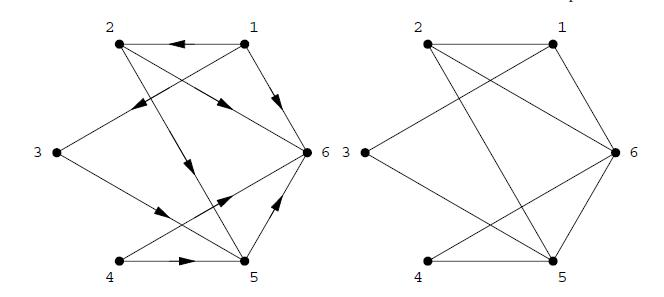
\includegraphics[width= 0.9 \linewidth]{Figuras/figura3.jpg}
\caption[Exemplo de grafos dirigidos e não dirigidos]{Exemplo de grafos
dirigidos e não dirigidos, ambos, com 6 vértices e
9 arestas. Retirada \cite{KlGo06}.}
\label{fig:ExemploGrafos}
\end{figure}

\begin{figure}[htb]
 \centering
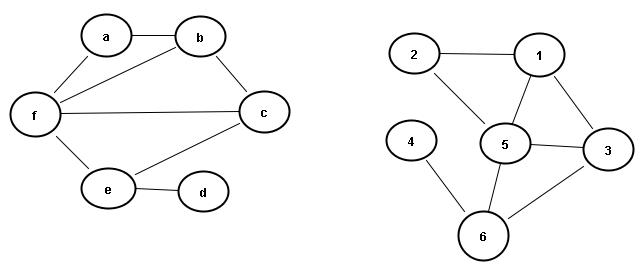
\includegraphics[width= 0.9 \linewidth]{Figuras/figura4.jpg}
\caption [Exemplo de dois grafos isomorfos]{Exemplo de dois grafos isomorfos. A
correspondência é dada pela função
$\{(a \rightarrow 2),(b \rightarrow 1),(c \rightarrow 3),(d\rightarrow
4),(e \rightarrow 6),(f \rightarrow 5)\}$}
\label{fig:ExemploGrafosIsomorfos}
\end{figure}

 A distância entre $x$ e $y$ é definida como o menor comprimento do caminho
para unir $x$ e $y$. O caminho em que as extremidades coincidem, ou seja, $x_0 =
x_l$ é denominado ciclo.

Um grafo é dito conexo se, para cada par de nós distintos $(x, y)$, existe um
caminho que os junta.  Uma árvore é um grafo conexo
sem ciclos.

\begin{figure}[!h]
 \centering
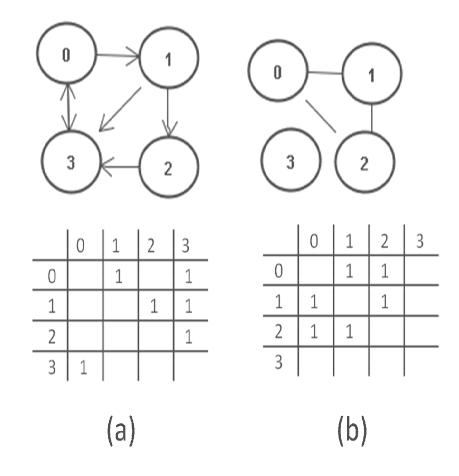
\includegraphics[width= 0.4 \linewidth]{Figuras/figura6.jpg}
\caption[Matriz de adjacência] {(a) Matriz de adjacência de um grafo dirigido.
(b) Matriz de adjacência de um grafo não dirigido.}
\label{fig:ExemploGrafoDirigido}
\end{figure}


Um grafo G de ordem N pode ser representado por uma matriz de adjacência $NxN$,
cujos elementos $a_{i,j}$ são determinados pela seguinte relação:
$a_{i,j}\left\{  \begin{array}{rcl}
1 & \rightarrow & (i,j) \in A \\ 
0 & \rightarrow & (i,j) \mbox{\hspace{.3em}}\mathcal{69}\mbox{\hspace{.3em}} A 
\end{array}\right.$


Essas propriedades dos grafos são importantes para a compreensão de redes
aleatórias. 

\subsection{Teoria dos Grafos Aleatórios-O Modelo de Erdõs e Rényi}

Em redes com topologia complexas, os princípios de organização são
desconhecidos. Por esse motivo os grafos
aleatórios são usados em seu estudo, pois suas arestas são distribuidas
aleatoriamente. A teoria de
grafos aleatórios foi introduzida pelos matemáticos húngaros Paul Erdõs e Alfred
Rény.


No modelo de Erdõs e Rényi, um grafo aleatório com $N$ nós conectados possui
$n$ arestas que são escolhidas aleatoriamente a partir de $\frac{N(N-1)}{2}$
possibilidades.  Assim o número possível de grafos com $N$ nós e $n$ arestas é
dada pela combinação simples $C^n_{\left[\frac{N(N-1)}{2}\right]}$, formando um
espaço probabilidade em que cada realização é equiprovável. O número esperado de
arestas, denotado por $E(n)$, é determinado de acordo com uma probabilidade de
ocupação $p$, definida como uma função do tamanho do sistema, onde $p$
representa a fração das arestas que estão presentes a partir de
$\frac{N(N-1)}{2}$ possibilidades.  Assim, o valor esperado do número total de
arestas é $E(n)=p \cdot \left[ \frac{N(N-1)}{2} \right]$. Em um grafo totalmente
conectado $p\rightarrow 1$.

A probabilidade de distribuição desse processo de um grafo
$G_o$ com $N$ nós é dado pela distribuição binomial:   $P(G_o)
= p^n(1-p)^{\frac{N(N-1)}{2} - n}$. A teoria dos grafos aleatórios estuda as
propriedades do espaço probabilidade dos grafos com $N$ nós,  $N \rightarrow
\infty$.

Em grafos com valores crescentes de $N$ e mesmo valor de $P$, conterá mais
arestas.

A maior descoberta de Erdõs e Rényi foi que muitas propriedades importantes de
grafos aleatórios aparecem de repente, denominadas genericamente como
propriedades emergentes
$Q$. Essas tais propriedades possuem uma probabilidade crítica $p_c(N)$. A
probabilidade que um grafo com $N$ nós conectado com probabilidade $P=p(n)$
tenha propriedades $Q$ é:

\begin{equation}
 \lim_{N\rightarrow \infty}P_{N,p}(Q)=\left\{\begin{array}{rcl}0 &
\mbox{se}&  \frac{p(N)}{p_c(N)}\rightarrow 0\\1 & \mbox{se}&
\frac{p(N)}{p_c(N)}\rightarrow \infty\end{array}\right.
\end{equation}

Essa probabilidade crítica é familiar em percolação.

\subsection{Subgrafos}

A 1$^a$ propriedade de grafos aleatórios estudada por Erdõs e Rényi (1959) foi a
emergência de subgrafos. Um grafo $G_1$ com um conjunto de $P_1$ nós $E_1$
arestas, é um subgrafo de um grafo aleatório $G=\{P,E\}$, se
todos os nós de $P_1$ são nós de $P$ e todas as arestas de $E_1$ são também
arestas de $E$. 

Os subgrafos completos de ordem $K$ possuem  todas as possíveis
$\frac{k(k-1)}{2}$ arestas conectadas. Para se determinar a probabilidade
crítica $P_c(N)$ que marca o aparecimento de subgrafos com $K$
nós e $L$ arestas, utiliza-se o seguinte processo; seja um grafo aleatório
$G=G(N,P)$ e um sub- grafo $F$ com ($K$,$L$). A principio $G$
pode conter diversos subgrafos $F$. Sabemos que os $K$ nós podem ser escolhidos
a partir de $N$ nós de $C_N^K$ maneiras e as $L$ arestas são conectadas com
probabilidade $P^L$. Permutando os $K$ nós é possível obter $K!$  novos grafos
(o valor correto é $\frac{K!}{a}$, onde $a$ é o numero de grafos que são
isomórficos). Assim o número esperado de subgrafos $F$ contidos em $G$ é:

\begin{equation}
E(X)=C^K_N\frac{K!}{a}P^L \cong \frac{N^KP^L}{a}
\end{equation}

A equação indica que se $P(N)N^{\frac{K}{L}}\rightarrow 0$, com $N\rightarrow
0$,
o
número esperado de subgrafo $E(X)\rightarrow 0$. Contudo,o número médio de
subgrafo é finito se
$P(N)=cN^{-\frac{K}{L}}$,  denotado por
$\lambda =\frac{c^L}{a}$, indicando que a função pode ter probabilidade crítica.

A probabilidade que $G$ contenha pelo menos um subgrafo $F$ é dado por:

\begin{equation}
P_p(G\supset F)=\sum_{r=1}^\infty P_p(X=r)=1-e^{-\lambda}
\end{equation}

Para valores de $P$ satisfazendo $PN^{\frac{k}{L}}\rightarrow \infty$ a
probabilidade $P_p(G\supset F)$ converge para 1. Assim a probabilidade crítica
que cada grafo contenha um subgrafo com $K$ nós e $L$ arestas é representada
por: 

\begin{equation}
P_c(N)=cN^{-\frac{K}{L}}
\end{equation}



\subsection{Distribuição dos Graus}

Em 1959, Erdos e Rényi, foram os primeiros a estudar o grau máximo e mínimo da
distribuição de um grafo aleatório.  Em um grafo aleatório com probabilidade de
conexão $P$ e grau $k_i$, o nó $i$ segue a distribuição binomial com
parâmetros $N - 1$ e $P$:

\begin{equation}
P(k_i=k)=C_{N-1}^k p^k(1-p)^{N-1-k},
\label{eq:distribuicao-dos-graus}
\end{equation}

ou seja, o número de maneiras em que $k$ arestas podem ser
adicionadas a partir de um determinado nó.  No estudo do grau de distribuição de
um grafo é necessário estudar o número de nós com grau $k$, $X_k$. Logo o
principal objetivo é determinar a probabilidade em que $X_k$  assume um
determinado valor $P(X+k=r)$.

O valor esperado de número de nós com grau $k$ é $E(X_k) = NP(k_i=k) =
\lambda_k$.

Substituindo em \ref{eq:distribuicao-dos-graus} tem-se que:

\begin{equation}
\lambda_k=NC_{N-1}^k p^k(1-p)^{N-1-k}
\end{equation}


Na derivação da condição de existência de subgrafos, a distribuição de
$X_k$ valores, $P(X_k = r)$, aproxima-se da distribuição de Poisson:

\begin{equation}
\label{eq:poisson}
P(X_k=r)=e^{-\lambda_k\frac{\lambda_k^r}{r!}}
\end{equation}

Como a distribuição de Poisson decai rapidamente para valores maiores de $r$, a
equação \ref{eq:poisson} implica que $X_k$ não diverge muito do resultado
aproximado $X_k=NP(k_i=k)$ ,  válido somente se os nós são independentes. Logo a
distribuição binomial é uma boa aproximação da distribuição do grau de um grafo
aleatório.

\begin{equation}
\label{eq:poisson2}
P(k)=C_{N-1}^kp^k(1-p)^{N-1-k}
\end{equation}

Para $N$ grande a equação \ref{eq:poisson2}, pode ser substituída pela
distribuição de Poisson

\begin{equation}
\label{eq:distribuicao-poisson}
P(k)\approx e^{-pN\frac{(pN)^k}{k!}}=e^{-\langle k \rangle \frac{\langle
k\rangle^k}{k!}}
\end{equation}

\subsection{Conexão de Diâmetro}

O diâmetro de um grafo é definido como a distância máxima entre qualquer par de
seus nós. Em um grafo desconectado (composto por vários clusters isolados) o
diâmetro é infinito. Mas, pode também ser definido pelo diâmetro máximo de seus
clusters. Geralmente, em grafos aleatórios, o diâmetro é pequeno, mesmo para
valores de $p$ não muito pequenos. A quantidade de nós
a partir de certo nó em uma distância $l$  não é menor que $\langle k\rangle$.
Assim, igualando
$\langle k\rangle^l$ com $N$, o diâmetro é proporcional
$\frac{\ln(N)}{\ln(\langle k \rangle)}$. Ou seja, depende do logaritmo sobre o
número de nós.

Quase todos os grafos com o mesmo $N$ e $P$ têm
precisamente mesmo diâmetro. Quando esses diâmetros de grafos com o mesmo $N$ e
$P$ variam, esse valor geralmente concentra-se em torno de
$d=\frac{\ln(N)}{\ln(pN)}=\frac{\ln(N)}{\ln(\langle k \rangle)}$.

Outra forma de caracterizar a propagação de um grafo aleatório é o cálculo da
distância média entre quaisquer pares de nós, definida por $l_{rand}\sim
\frac{\ln(N)}{\ln(\langle k \rangle)}$.

\subsection{Coeficiente de Clustering}

As redes complexas possuem um alto grau de clusterização. Considere a seguinte
hipótese: seja um nó em um grafo aleatório e seus vizinhos mais próximos, a
probabilidade que dois desses vizinhos estejam conectados é igual a
probabilidade que dois nós selecionados aleatoria\-mente estejam conectados.
Logo o coeficiente de agrupamento de um grafo aleatório é
$C_{rand}=p=\frac{\langle k \rangle}{N}$.



Na seção abaixo, será apresentado o modelo de \emph{random walk}. No contexto da
literatura da economia, para a descrição do comportamento da series temporais do
mercado financeiro.

\section{Passeio Aleatório (\emph{Random Walk})}

Em 1990, Louis Bachelier propôs em sua tese de doutorado que a trajetória das
séries
temporais dos índices do mercado de ações seguia um passeio aleatório
(\emph{random walk}) \cite{So02}. O conceito de \emph{random walk} é simples e
suas aplicações não se restringem somente à área de finanças, havendo diversas
utilizações como, por exemplo, na descrição de fenômenos naturais. Em sua versão
mais simples, o \emph{random walk} pode ser simulado através de jogadas de uma
moeda. Sornette \cite{So02} simula a trajetória dos preços do mercado de ações
através de sorteios de moedas no computador para decidir a mudança de preço, ou
seja, se sobe ou desce.

Os resultados obtidos nesse mercado artificial foram comparados com os índices
de mercados reais. Baseando-se nas análises estatísticas observadas,
Sornette reforça a hipótese que o modelo de \emph{random walk} descreve bem as
mudanças dos preços no mercado de ações.

Logo, as variações dos preços são realmente como lançamento aleatório de
moedas, ou seja, equivale a dizer que é impossível saber a direção
dos  preços entre hoje e amanhã, ou entre duas datas quaisquer. A crença é
que essa aleatoriedade é alcançada por causa da participação ativa de
muitos investidores que objetivam o aumento máximo da riqueza, 
determinada com base em informações por
ele obtidas. Na seção abaixo, será dada uma definição formal do modelo de
\emph{random walk}.

\subsection{Definição}

Na definição de passeio aleatório simples em $Z$ podemos imaginar um indivíduo
que se desloca sobre uma reta, inicialmente na origem, dando passos de
comprimentos iguais $(l)$. Esse indivíduo se move nos sítios de $Z$ e a cada
instante pode pular de um ponto $x$ para um de seus próximos vizinhos $x + 1$ ou
$x - 1$, com probabilidade $p \in [0,1]$ de pular para o sítio à sua direita e
probabilidade $q=1-p$ para o sítio à sua esquerda.  A probabilidade $P_N(m)$  de
que o indivíduo se encontre na posição $y=ml$, depois de ter dado $N$ passos, é
demonstrada abaixo.


A relação $(p\dots p)(q\dots q)=p^{N_1}q^{N_2}$ representa a probabilidade de
uma determinada sequência de $N$ passos, com  $N_1$ passos para direita e $N_2$
passos para esquerda. O número total de sequências desse tipo é obtido pelo
fator combinatório $\frac{N!}{N_1!N_2!}$.

Logo, para um total de $N$ passos a probabilidade de dar $N_1$ passos para
direita e $N_2$ passos para esquerda é dada pela distribuição binomial:

\begin{equation}
\label{eq:distribuicao-binomial}
W_N(N_1)=\frac{N!}{N_1!N_2!}p^{N_1}q^{N_2}
\end{equation}

Como $p+q=1$ e $N_1+N_2=N$. Pela definição $m=N_1-N_2$; Logo é fácil mostrar
que $P_n(m)$ é

\begin{equation}
\label{eq:distribuicao-binomial2}
P_N(m)=\frac{N!}{\left(
\frac{N+m}{2}\right)!\left(\frac{N-m}{2}\right)!}p^{\frac{N+m}{2}}q^{\frac{N-m}{
2}}
\end{equation}

O valor médio de $N_1$ é dado pela seguinte relação:

\begin{eqnarray}
\label{eq:valor-medio}
\langle N_1 \rangle &=& \sum_{N_1=0}^N N_1 W_N(N_1) \nonumber\\
&=& \sum_{N_1=0}^N N_1\frac{N!} {N_1!N_2!} p^{N_1}q^{N_2}\nonumber\\
&=& p \frac{d}{dp} \sum_{N_1=0}^N \frac{N!}{N_1!N_2!}p^{N_1}q^{N_2}\nonumber\\
&=& p\frac{d}{dp}(p+q)^N=pN(p+q)^{ N-1}\nonumber\\
&=& pN
\end{eqnarray}

Através de um procedimento análogo ao \ref{eq:valor-medio} temos o valor
médio
de $\langle N_2 \rangle = qN$. Para o cálculo da dispersão em relação à média,
é feito o mesmo procedimento, observando que:

\begin{eqnarray}
\label{eq:valor-medio-N2}
\langle N_1^2 \rangle &=& p\frac{d}{dp}\left\{
p\frac{d}{dp}\left[\sum_{N_1=0}^N \frac{N!}{N_1!N_2!}p^{N_1}q^{N_2} \right]
\right\} \nonumber \\
&=& \left( p\frac{d}{dp}\right) \{ pN(p+q)^{N-1}\} \nonumber \\
&=& pN+p^2N(N-1)
\end{eqnarray}

Assim temos:

\begin{equation}
\label{eq:valor-medio-N2-2}
\langle (\Delta N_1)^2 \rangle = \langle N_1^2 \rangle - \langle N_1 \rangle^2
= Npq
\end{equation}

Logo, o desvio padrão é $\sqrt{Npq}$. As expressões acima estão explicadas com
mais detalhes em \cite{Sa97}.

O \emph{random walk} possui propriedade de auto-similaridade, que será definida
na próxima seção a partir da geometria fractal.

\section{Geometria Fractal}

Historicamente, o interesse na geometria tem sido estimulado pelas
diversas aplicações; na descrição da natureza, por exemplo: a elipse é associada
às  órbitas planetárias, a esfera à forma da Terra etc. Contudo, as geometrias
da elipse e da esfera não podem ser aplicadas com exatidão a estas
situações físicas, pois as órbitas não são perfeitamente elípticas e a Terra
não é realmente esférica. No passado, a preocupação da matemática era com
os conjuntos e funções cujos métodos de cálculo poderiam ser aplicados.
As funções que não eram regulares eram ignoradas, consideradas apenas
como curiosidades, e vistas raramente como uma classe à qual uma teoria
poderia ser aplicável à descrição da natureza.

Nos últimos anos, essa postura vem mudando pela necessidade em reproduzir
com alto grau de exatidão estruturas complexas observadas na natureza, e
a matemática de objetos irregulares começou a ser explorada. As
formas apresentadas fornecem representações mais exatas de fenômenos do que
a geometria clássica fornecia. Em 1960, vários pesquisadores passaram a estudar
e analisar tais formas geométricas. Em 1975, Benoit Mandelbrot,
matemático polonês considerado pai da geometria de objetos
irregulares, difundiu amplamente seu estudo e a nomeou como ``Geometria
Fractal''. Sua intenção, ao criar a palavra ``Fractal``, foi unir numa só
palavra
uma classe de objetos conhecidos como ‘monstros matemáticos’, que assombraram
a carreira de muitos cientistas. O termo surgiu do latim, do adjetivo
\emph{fractus}: fragmento, fração.

Fractais são formas geométricas abstratas de uma beleza incrível, com
padrões complexos que se repetem indefinidamente, mesmos limitados a uma área
finita. Por exemplo, ao tirar uma foto  de uma pequena 
parte de uma couve-flor, observar-se-á que o pequeno pedaço é semelhante ao
todo.
Tal fenômeno está presente na natureza, como na estruturas das plantas,
das montanhas, do cérebro, etc \cite{Ja08}.

A união da teoria do Caos com a geometria  fractal tornou-se uma nova
fronteira da ciência, cujas aplicações se estendem a diversos ramos
do conhecimento: economia, física, matemática, biologia etc\dots A
literatura recente da física mostra uma variedade de objetos que são
descritos através de fractais, como nuvens, superfícies topográficas, a
orla costeira, turbulência de fluidos, e assim por diante \cite{Fa03}.

Pelas diversas formas de se apresentar, é extremamente difícil definir fractal
de um modo que atenda a todas as espécies de construção. Mandelbrot definiu
um fractal como um conjunto de Hausdorff \cite{Fa03} cuja dimensão é maior que
sua dimensão topológica e menor que a de imersão, ou seja, um conjunto $F$
é fractal se, em $F$, $D > DT$, sendo $D$ a dimensão fractal e $DT$ a dimensão
topológica do conjunto $F$.

Kenneth Falconer \cite{Fa03} propõe uma definição menos rigorosa para os
fractais: uma dada figura será considerada fractal se possuir uma estrutura fina
em qualquer escala e se sua construção for feita por outra função, que não
seja analítica,  por outra linguagem, que não seja a geométrica tradicional.
Essa figura deve também possuir alguma espécie de auto-similaridade,
sua estrutura deve ser maior que a dimensão topológica, podendo ter uma lei
de formação simples ou, às vezes, obtida recursivamente.

\subsection{Conjunto de Cantor}

George Cantor propôs um conjunto, definido como o subconjunto dos
números reais. Tal construção definiu-se um dos mais conhecidos
conjuntos fractais, o terço médio de Cantor. Ele é construído a partir de um
intervalo de unidade por uma sequência de operações de eliminação. Abaixo é
exemplificada
sua construção: Seja $E_0$ o conjunto no intervalo real $[0,1]$. O conjunto
$E_1$ é obtido através da divisão de $E_0$ em três conjuntos iguais e
retirando-se o termo do meio, ou seja, $E_1$ consiste nos intervalos
$[0,\frac{1}{3}]$ e $[\frac{2}{3},1]$. Repetindo-se o mesmo procedimento para
$E_2 $ obtém os intervalos $[0,\frac{1}{9}]$, $[\frac{2}{9},\frac{1}{3}]$,
$[\frac{2}{3},\frac{7}{9}]$ e $[\frac{8}{9},1]$. Assim, em $E_k$ é obtido pelo
mesmo processo através do intervalo $E_{k-1}$. O processo é feito
sucessivamente até que o numero $k$ tenda ao infinito. O número de intervalos de
$E_k$ é $2^k$ com comprimento $3^{-k}$. Matematicamente, o conjunto terço médio
de Cantor $E$ é o intervalo $\cap_{k=0}^\infty C_k$.

\begin{figure}[!h]
 \centering
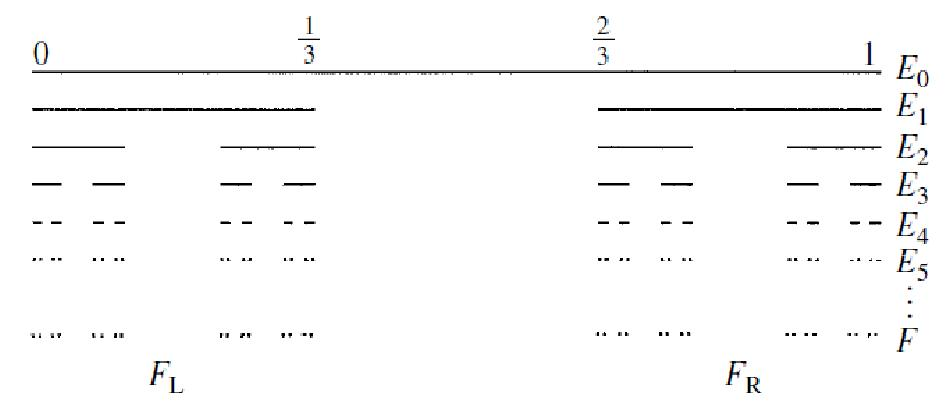
\includegraphics[width= 0.9 \linewidth]{Figuras/figura7.jpg}
\caption [Construção do conjunto fractal o terço médio de Cantor]{Construção do
conjunto fractal o terço médio de Cantor, em cada
passagem, o conunto $E_k$ é obtido através da divisão de $E_{k-1}$ em três
conjuntos iguais e retirando-se o termo do meio. Retirada de \cite{HuDo62}.}
\label{fig:Cantor}
\end{figure}

\subsection{Curva de Koch}

O matemático Niels Von Koch ficou famoso devido a um artigo que publicou em
1904, sobre uma curva sem tangentes e contínua em todos os pontos, conhecida
como curva de Koch. O procedimento para se obter a curva de Koch é similar ao do
conjunto de Cantor. Seja $E_0$ um segmento de tamanho unitário; o conjunto $E_1$
consiste na substituição do terço médio do segmento $E_0$ por um triângulo
equilátero sem a base. Para construção de $E_k$, é aplicado o mesmo processo em
$E_{k-1}$. Quando $k$ é grande, as curvas $E_{k-1}$ e $C_k$ diferem em pequenos
detalhes. O comprimento de $E_k$ é obtido pela relação
$\left(\frac{4}{3}\right)^k$, ou seja, quando $k$ tende ao infinito, $E_k$ tem
comprimento infinito, em uma área limitada.

\begin{figure}[!h]
 \centering
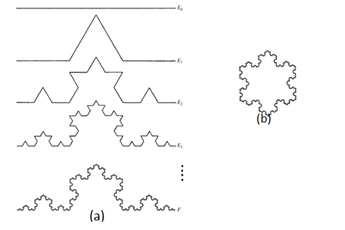
\includegraphics[width= 0.6 \linewidth]{Figuras/figura8.jpg}
\caption[Construção da curva de Koch]{(a) Construção da curva de Koch, em cada
passagem, o conjunto $E_k$
consiste na substituição do terço médio do segmento $E_{k-1}$ por um triângulo
equilátero sem base. (b) Curva de Koch construída a partir da estrela de Davi.
Retirada de \cite{HuDo62}.}
\label{fig:Koch}
\end{figure}

\subsection{Dimensão Fractal}

Um dos principais problemas em matemática é determinar o que é dimensão e suas
propriedades. Podemos enumerar diversas definições de dimensão, como euclidiana,
de
Hausdorff, fractal, topológica, etc. A dimensão topológica, $d_t$, é definida
como a soma de uma unidade à dimensão euclidiana do menor conjunto que, ao ser
subtraído de
outro conjunto conexo, deixa-o desconexo. Por definição, $d_t$ de um ponto é
igual a 0; desse modo, ao retirarmos um ponto de uma reta obteremos duas
semi-retas e, portanto, a $d_t$ de uma reta é igual a 1, $d_t$ de um plano é
igual a 2, etc\dots Já a dimensão euclidiana, $d$, corresponde à dimensão de
imersão: $d=0$ é um ponto, $d=1$ uma linha, etc.

A noção de dimensão é fundamental para a geometria fractal, e caracteriza
 como um objeto fractal preenche o espaço. A definição de Mandelbrot,
utiliza a dimensão de Hausdorff, usada no conceito matemático da medida
\cite{Fa03}.

Uma maneira de definir a dimensão fractal é utilizando o método contagem de
caixas. A medida $M$ de um objeto pode
ser feita através da contagem de caixas de exclusão linear $\rho$:

\begin{equation}
\label{eq:contagem-caixas}
M_d=N(\rho)\rho^d,
\end{equation}
onde $N(\rho)$ é o menor número de caixas de $d$-dimensionais, com extensão
linear $\rho$ suficiente para recobrir todo o objeto. Para objetos fractais, 
$N(\rho)\sim \rho^D$, para $\rho \rightarrow 0$, de tal modo que:

\begin{equation}
\label{eq:contagem-caixas2}
N(\rho)\rho^d\rightarrow \left\{\begin{array}{rcl} \infty, & \mbox{se} & d<D \\
0, & \mbox{se} & d>D
\end{array}\right.
\end{equation}

O valor da dimensão fractal pode ser obtido numericamente pela expressão:

\begin{equation}
\label{eq:contagem-caixas3}
D=\lim_{\rho \rightarrow 0}\frac{\ln N(\rho)}{\ln (\frac{1}{\rho})}
\end{equation}

Quando esse limite existir.

\subsection{Auto-Similaridade e Auto-Afinidade}

Fractais são constituídos por partes que são, de alguma forma, similares
ao todo. Esta característica é denominada auto-similaridade. A
auto-similaridade não é apenas uma propriedade dos fractais, pode ser utilizada
também para defini-los. Auto-similaridade é uma propriedade de simetria do
sistema, indicando invariância sob uma transformação isotrópica. Seja $D$ um
subconjunto fechado de $R^n$. Uma função $S:D\rightarrow D$ é definida uma
contração em $D$ se existe um número $c$ tal que $0<c<1$ e
$|S(x)-S(y)|\leq c|x-y| \mbox{\hspace{.3em}} \forall \mbox{\hspace{.3em}} x, y
\in D$. Qualquer contração é continua. 

No caso em que $|S(x)-S(y)|=c|x-y|$, o conjunto de transformação $S$ define
geometricamente conjuntos auto-similares.  Assim o conjunto é idêntico a uma
parte do
sistema original.  O terço médio de Cantor e a curva de Koch são exemplos de
figuras auto-similares. No caso de um objeto auto-afim, sua transformação de
escala é anisotrópica, ou seja, são usados diferentes fatores de redução na
dilatação de um objeto para manter a invariância de escala. Uma transformação
afim $S:R^n \rightarrow R^n$ é definida como $S(x)=T(x)+b$, na qual $T$ é uma
transformação em $R^n$ (representada por uma matriz $nxn$) e $b$ um vetor em
$R^n$. Assim, a transformação afim geral $S$ é uma combinação de translação,
rotação, dilatação e, às vezes, reflexão. Os conjuntos auto-similares são um
caso particular dos conjuntos auto-afins.

Para quantificar o grau de auto-afinidade, utiliza-se o expoente de Hurst.

\section{Expoente de Hurst}

Em sistemas descritos por funções $h(x)$ que apresentam auto-afinidade, temos a
seguinte relação:

\begin{equation}
\label{eq:rugosidade-hx}
h(x) \sim b^{-H}h(bx),
\end{equation}
na qual $H$ é o expoente de Hurst,  ou expoente auto-afim, que fornece uma
medida da como a rugosidade da função $h(x)$ varia com a escala. A equação é
obtida diretamente da definição de função auto-afim, na qual reescalamos a
direção $x$ por $bx$ e a direção de $h$ por $b^Hh$.

O expoente de Hurst é aplicável em diversas situações. Como o tema dessa
dissertação é referente à economia, será considerado o ponto de vista de sua
aplicação  no mercado financeiro.

Mandelbrot foi o primeiro a observar e considerar um comportamento de longa
memória em ativos de retorno. Essa característica tem intrigado os acadêmicos e
os profissionais dos mercados econômicos ao longo dos anos \cite{CaTa08}.
Tal interesse se deve ao fato de que resultados relacionados à existência da
propriedade de memória de longo alcance não servem apenas como evidência da
forma fraca da hipótese do mercado eficiente, mas também estão intimamente
relacionados à previsibilidade dos preços dos ativos. Se essas propriedades de
memória de longo alcance, presentes nas séries temporais dos índices dos
mercados financeiros, for persistente, a hipótese do \emph{random walk} não é
válida,
 invalidando, consequentemente, a hipótese do mercado eficiente. O expoente de
Hurst é proposto na literatura para classificar os índices das bolsas de valores
dos países e como uma medida da eficiência do mercado. Assim, através desta
metodologia, torna-se possível avaliar o grau de dependência das propriedades de
memória de longo alcance das séries temporais
\cite{CaTa08,CoVa03,CaTa04,CaCaSt04,LiAnFi09}.

Através do cálculo do expoente de Hurst $(H)$, observa-se que para
$H=\frac{1}{2}$ tem-se uma série decorrelacionada, e valores diferentes indicam
a existência de correlações de longo alcance. Quando $0.5< H <1$, a série é
positivamente correlacionada e apresenta persistência. No caso de $0< H <0.5$, a
série é negativamente correlacionada e apresenta anti-persistência. Uma série
anti-persistente possui a característica de ``reversão à média'', o que
significa que uma subida no valor da série é mais provavelmente seguida de uma
descida no valor e vice-versa. Quanto mais próximo de 0 estiver, maior a
intensidade da ``reversão à média''. Já a série persistente é uma série em que a
tendência se mantém, a direção (subida ou descida, comparado ao último valor) do
próximo valor será, provavelmente, a mesma do valor corrente.

O cálculo do expoente de Hurst pode ser feito por diversos métodos. Abaixo são
apresentados o \emph{Rescaled Range Analisis} (R/S) e o \emph{Detrended
Fluctuation Analysis} (DFA).

O método R/S é o mais conhecido e usado devido à sua simplicidade. Pode ser
descrito da seguinte maneira: o valor do índice da ação é representado por
$X(t)$ referente ao tempo $t$, e o logaritmo do retorno é representado por
$r(t)=\ln \left( \frac{X(t+1)}{X(t)}\right)$; a média dos retornos é definida
por $\overline{r}_n$, sendo obtida pelo somatório dos retornos, dividido pelo
tempo, ou seja, $\overline{r}_n=\frac{1}{t}\sum_n r(n)$, em que $n$ representa
o. número de pontos. O desvio é
$r(t)-\overline{r}_n$. A amplitude do desvio médio é:

\begin{equation}
\label{eq:amplitude-desvio}
R_n = \mbox{\emph{max}}\sum_{k=1}^n
(r(k)-\overline{r}_n)-\mbox{\emph{min}}\sum_{k=1}^n (r(k)-\overline{r}_n)
\end{equation}

O desvio padrão estimado é:

\begin{equation}
\label{eq:desvio-padrao-estimado}
S_n = \left[ \frac{1}{n}\sum_t (r(t)-\overline{r}_n)^2 \right]^{\frac{1}{2}}
\end{equation}

O método $(R/S)_n$ é dado pela divisão de $R_n$ por $S_n$. O valor do expoente
de Hurst (denotado pela letra $H$) é obtido pela relação $(R/S)_n=(n/2)^H$.

Por sua característica assintótica, o método R/S deve ser utilizado somente para
séries temporais longas. Um método alternativo para R/S é o DFA, uma técnica
mais robusta e eficiente. O cálculo do DFA para séries temporais financeiras
\cite{CoVa03} é explicado a seguir.

A sequência dos desvios médios é dada por
$D(t)=\sum_{t=1}^T(r(t)-\overline{r})$. Dividindo a série $D(t)$ em $N$
intervalos não sobrepostos $I_n$, todos de tamanho $p$, onde $n=0,1,\dots,N-1$,
em que $N$ é a parte inteira de $T/p$. Para cada $t$ pertencente ao intervalo
$I_n$, é possível obter uma reta de tendência local definida da seguinte forma:

\begin{equation}
\label{eq:reta-tendencia-local}
Y_p(t)=a_n+b_n\cdot t
\end{equation}

Onde os valores de $a_n$ e $b_n$ são encontrados pelo método de mínimos
quadrados ordinários. Usando como parâmetro $D(t)$ no intervalo $I_n$, a função
de flutuação $F_t$ é definida pelo desvio padrão:

\begin{equation}
\label{eq:desvio-padrao-flutuacao}
F(p)=\sqrt{\frac{1}{T}\sum_{t=1}^T [D(t)-Y_p(t)]^2}
\end{equation}

O valor do expoente de Hurst $H$ é obtido pela relação $F(p)\sim p^H$. O
expoente $H$ é calculado como a inclinação da reta ajustada no gráfico log-log,
usando o método dos mínimos quadrados ver no gráfico na figura
\ref{fig:grafico1}

\begin{figure}[!h]
 \centering
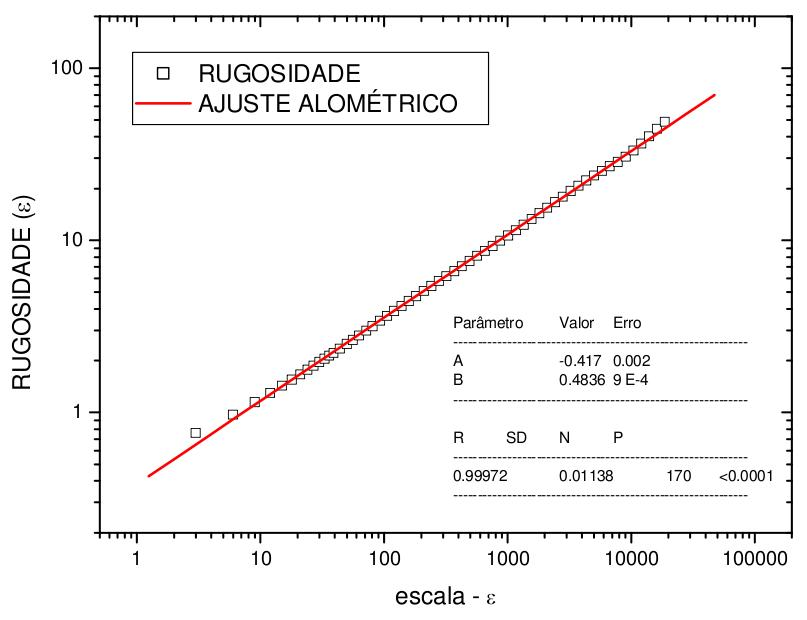
\includegraphics[width=.7\linewidth]{Figuras/figura9.jpg}
\caption[O expoente de Hurst no \emph{randow walk}] {Valor do expoente de Hurst
para uma amostra \emph{randow walk} com
100.000 pontos
pelo método DFA.}
\label{fig:grafico1}
\end{figure}


Cajueiro e Tabak \cite{CaTa08} classificaram os índices de mercados reais
utilizando o expoente de Hurst de séries temporais, empregando duas metodologias
diferentes,
sendo uma delas o método do R/S. Segundo Cajueiro e Tabak \cite{CaTa08, CaTa04},
o valor do expoente de Hurst nos mercados de ações em mercados desenvolvidos --
onde é válida a hipótese de mercado eficiente -- deve estar próximo de $H=1/2$.

O cálculo do expoente de Hurst foi empregado em 41 países da Europa, Asia,
America Latina e o Oriente Médio, no período de 1999 a 2005 \cite{CaTa08}. Com
 média de 1776 observações. Todos os índices de países foram estudados para o
mesmo período de tempo. Nos testes foram calculados o nível de significância
referente a 5\% (valores menores que 0,05 indicam rejeição da hipótese nula)
o valor do expoente Hurst igual a 0,5.

A média do expoente de Hurst, através do método R/S, para mercados desenvolvidos
foi 0,561, e para os mercados emergentes 0,597. Na América latina e Ásia, o
valor médio do expoente Hurst, foi 0,60 e 0,584, respectivamente, sugerindo
menor grau de previsibilidade na economia asiática. No entanto, o expoente de
Hurst na Tailândia foi de 0,621, o que sugere que as comparações regionais devem
ser feitas com cuidado. O menor valor encontrado foi, 0,519, nos Estados Unidos
e o maior foi  0,656 no Peru.

Em muitos países a hipótese nula da ausência de longa dependência foi
rejeitada. Nos países de mercados emergentes o $p$ - valor foi menor do que
0,05, indicando assim rejeição da hipótese nula do expoente Hurst ser igual a
$(1/2)$.  Já nos países desenvolvidos, em apenas quatro países, a hipótese
nula foi
rejeitada.  Confirmando  que o expoente de Hurst em mercados
desenvolvidos deve-se aproximar de $(1/2)$. Esses resultados empíricos sugerem
que
os
índices de mercados emergentes possuem, em média, maior dependência de longo
alcance do que os retornos dos mercados desenvolvidos. 

\chapter{Modelo}\label{modelo}

O objetivo desse capítulo é formalizar o modelo de mercado financeiro artificial
que reproduza propriedades estatísticas encontradas em séries financeiras reais.
Neste trabalho, consideraremos o mercado representado por um autômato celular,
considerando-se dois tipos de rede, a regular e a rede aleatória.  O modelo
proposto é composto por agentes com até quatro tipos de comportamento diferentes
imitadores, anti-imitadores, indiferentes e o imitador do mais rico. O
investidor possui três
estados diferentes: comprar, manter e vender, sendo representadas pelos
estados 0,1e 2, respectivamente. Abaixo será formalizado o modelo.

\section{Mercado Financeiro representado por um autômato celular}

A representação do mercado por um autômato celular é feita em uma rede de duas
dimensões, com condições periódicas de contorno, onde cada sítio representa um
investidor. A extensão linear da rede é $L=100$, com $N=10000$ sítios
(investidores). As regras de evolução são determinísticas ou probabilísticas. A
variável $S^t(i,j)$
denota a opção do  investidor no sítio $(i,j)$, no tempo $t$. Utilizamos a
vizinhança de Moore, com oito vizinhos, para rede regular. . As regras de
evolução serão diferentes para cada caso de comportamento de investimento. De um
modo geral, as regras são determinadas pelo estado predominante da vizinhança em
um dado passo de tempo. Na rede regular, a escolha do investidor no tempo  $t+1$
 é uma função do estado majoritário entre os vizinhos no tempo $t$, representada
pela equação: 



\begin{eqnarray}
S^{t+1}(i,j) & = & f(S^t(i-1,j-1),S^t(i-1,j),S^t(i-1,j+1),S^t(i,j-1),\nonumber
\\
& & S^t(i,j+1),S^t(i+ 1,j-1),S^t(i+1,j),S^t(i+1j+1))
\end{eqnarray}

\begin{figure}[!h]
\centering
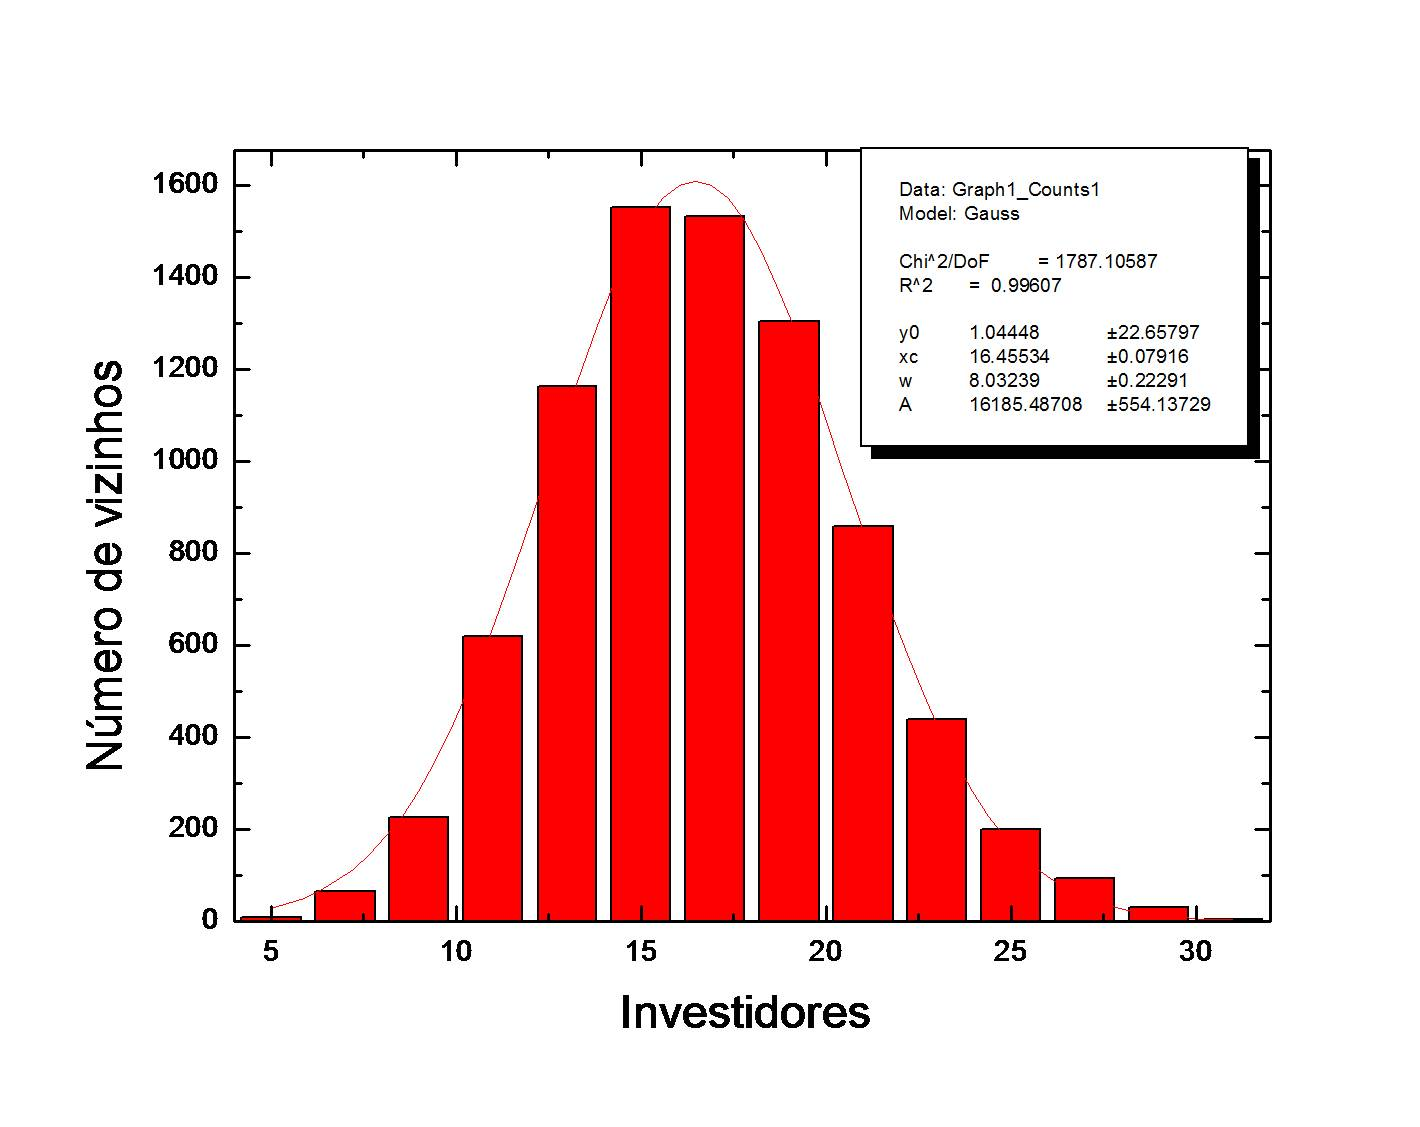
\includegraphics[width=0.8\linewidth]{Figuras/0.jpg}
 \caption{Distribuição do número de vizinhos (grau) de cada investidor
(nó) para um rede aleatória com $p=0.002$ e $L=90$.}
\end{figure}

Nas redes aleatórias, baseamos a construção da rede no modelo de Erdõs e Rényi.
A quantidade esperada de nós conectados é definida por  $E(n)=p \cdot \left[
\frac{N(N-1)}{2} \right]$, onde $N$ é o número de nós e $p$ a probabilidade de
ocupação.  No nosso modelo, optamos pela escolha do valor de $p=0,002$, e o
número de vizinhos de cada nó, ou seja, o grau de cada nó variou aproximadamente
entre 5 a 30. Tal relação esta representada no histograma da figura 4.1, e como
esperado, segue uma distribuição gaussiana.

Nas redes aleatórias, o estado do investidor no tempo $t+1$ é uma
função do estado majoritário entre os vizinhos no tempo $t$, representado pela
equação:



\begin{equation}
S^{t+1}(i,j)=f\left( \sum_{0}^{n[i,j]} S^t(a,b) \right)
\end{equation}

Onde $n[i,j]$ é o número de vizinhos do investidor $S^t(i,j)$ e $S^t(a,b)$ são
os vizinhos de $S^t(i,j)$, que são relacionados pela matriz de adjacência:

\begin{equation}
 S^t(a,b)=\left\{ \begin{array}{rcl}
1 & \rightarrow & (a,b) \in A \\
0 & \rightarrow & (a,b) \not\exists \mbox{\hspace{.2em}} A
\end{array}\right.
\end{equation}

Onde A representa a vizinhança do investidor $S^t(i,j)$.

\subsection{Agentes e suas estratégias}

No nosso modelo os agentes representam os investidores em um mercado financeiro
onde compram, vendem ou mantém suas ações a partir de estratégias de acordo com
suas características psicológicas.

Foram considerados quatro tipos de comportamento para os investidores. No
primeiro tipo, denominado ``imitador'', a escolha do investidor será idêntica
à escolha predominante de sua vizinhança no caso empate, poderá ser
considerada o estado do investidor no tempo anterior ou o estado será 
manter dependendo das hipóteses representadas abaixo.

\begin{enumerate}
 \item[I.] existir um único máximo. 

\item[II.] se $C[0]=C[1]$ e $S^t(i,j)\neq 2$ ou se $C[2]=C[1]$ e $S^t(i,j)\neq
0$ ou se $C[0]=C[2]$ e $C[0]>C[1]$
\end{enumerate}

Temos

\begin{equation}
S^{t+1}(i,j)=\left\{ \begin{array}{rl}
max[C[0],C[1],C[2]] & \mbox{se I for verdadeira} \\
S^t(i,j) & \mbox{se II for verdadeira} \\
1 &  \mbox{caso contrário}
\end{array}\right.
\end{equation}

Onde $C[i]$ com $i \in {0,1,2}$ representa a quantidade de vizinhos do sítio
$(i,j)$ que estão comprando, mantendo ou vendendo, respectivamente;

O segundo, denominado ``anti-imitador``, o investidor opta pelo contrário da
tendência predominante entre seus vizinhos. Se a escolha predominante for
manter, o anti-imitador escolherá, entre as escolhas comprar e vender, a menos
predominante. No caso de empate entre essas escolhas, poderá será considerada a
escolha do investidor no tempo anterior ou a escolha manter de acordo com a
função representada abaixo:

\begin{equation}
S^{t+1}(i,j)=\left\{ \begin{array}{rl}
min[C[0],C[2]] & \mbox{se\hspace{.7em}} C[0] \neq C[2] \\
S^t(i,j) & \mbox{se\hspace{.7em}} C[0]<C[1] \\
1 &  \mbox{caso contrário}
\end{array}\right.
\end{equation}

O terceiro tipo, denominado ``indiferente'', a escolha do investidor é
independente da tendência dos vizinhos, com probabilidade de 50\% de
mudança, sendo determinada aleatoriamente entre as três escolhas possíveis.

\begin{equation}
S^{t+1}(i,j)=\left\{ \begin{array}{rl}
0 & \mbox{se\hspace{.7em}} 0 \leq \alpha < \frac{1}{6} \\
1 & \mbox{se\hspace{.7em}} \frac{1}{6} \leq \alpha < \frac{1}{3} \\
2 & \mbox{se\hspace{.7em}} \frac{1}{3} \leq \alpha < \frac{1}{2} \\
S^t(i,j) &  \mbox{caso contrário}
\end{array}\right.
\end{equation}

Em que $\alpha$ representa um número aleatório no intervalo $[0,1]$.

O quarto tipo, denominado ``imitador do mais rico``, cada investidor irá imitar
o jogador de sua vizinhança que obteve o maior lucro, ou seja, que possui mais
dinheiro até o momento analizado: 

\begin{equation}
S^{t+1}(i,j)=S^t(a,b)
\end{equation}

Onde o investidor $(a,b)$ é determinado pela equação abaixo:

\begin{eqnarray}
S(a,b)&=&Max(D^t(i-1,j-1),D^t(i-1,j),D^t(i-1,j+1),D^t(i,j-1),\nonumber \\
&& D^t(i,j+1),D^t(i+1,j-1),D^t(i+1,j),D^t(i+1,j+1))
\end{eqnarray}

onde $D^t(i,j)$ representa a quantidade de dinheiro no tempo $t$. 
\subsection{Dinâmica  do índice do mercado }

O índice do mercado de ações é afetado a cada passo pelo comportamento
dos investidores, ou seja, pela lei da procura e oferta.  O
valor do índice inicial é 100,00.

A função definida como $Sindex[t]$ no tempo $t$ é
definida por:

\begin{equation}
Sindex[t]=\sum_{i=0}^{L-1}\sum_{j=0}^{L-1}(S^t(i,j)-1)
\end{equation}

O cálculo do índex, definida como $index[t]$ no tempo $t$ é definido como:

\begin{equation}
index[t]=index[t-1]+K\cdot Sindex[t]
\end{equation}

Onde $K$ é uma constante determinada.



\subsection{Quantidade de dinheiro e ações iniciais}

Duas situações serão consideradas. A primeira situação a quantidade de dinheiro
e ações é ilimitada. Na segunda situação a quantidade de dinheiro e ações
é limitada, sendo que cada investidor $(i,j)$ no tempo inicial começará com
R\$10.000 e 100 ações.

Para a segunda situação, foram criadas as seguintes regras: se a escolha
do investidor $(i,j)$ de acordo com seu tipo de comportamento fosse vender, no
tempo $t$, e sua quantidade de ações (representada por $A^t(i,j)$), nesse mesmo
tempo, fosse igual a zero, a sua escolha seria alterada para manter. Já no caso
em que a escolha do investidor $(i,j)$ de acordo com seu tipo de
comportamento fosse comprar, no tempo $t$, e sua quantidade de
dinheiro (representada por $D^t(i,j)$), nesse mesmo tempo, fosse igual menor do
que o preço atual do índice, a sua escolha mudaria para manter também.
Desse modo:

\begin{enumerate}
 \item[I.] $S^{t+1}(i,j)=0$ e $A^t(i,j)=0$ ou $S^{t+1}(i,j)=0$ e
$D^t(i,j)<index[t]$
\end{enumerate}

\begin{equation}
S^{t+1}(i,j)=\left\{ \begin{array}{rl}
1 & \mbox{se I for verdadeiro}\\
S^t(i,j) &  \mbox{caso contrário}
\end{array}\right.
\end{equation}

Em cada passo de tempo na situação 2, a quantidade de dinheiro $D^t(i,j)$ do
investidor $(i,j)$ é atualizada de acordo com suas escolhas.

\begin{equation}
D^{t+1}(i,j)=\left\{ \begin{array}{rl}
D^t(i,j)+index[t] & \mbox{se\hspace{.7em}} S^{t+1}(i,j)=0
\mbox{\hspace{.7em}e\hspace{.7em}} A^t(i,j)>0\\
D^t(i,j) & \mbox{se\hspace{.7em}} S^{t+1}(i,j)=1 \\
D^t(i,j)-index[t] & \mbox{se\hspace{.7em}}
S^{t+1}(i,j)=2\mbox{\hspace{.7em}e\hspace{.7em}} D^t(i,j) > index[t]\\
\end{array}\right.
\end{equation}

A quantidade de ações $A^t(i,j)$ do investidor $(i,j)$ também é atualizada de
acordo com suas escolhas.

\begin{equation}
A^{t+1}(i,j)=\left\{ \begin{array}{rl}
A^t(i,j)+1 & \mbox{se\hspace{.7em}} S^{t+1}(i,j)=2
\mbox{\hspace{.7em}e\hspace{.7em}} D^t(i,j)>index[t]\\
A^t(i,j) & \mbox{se\hspace{.7em}} S^{t+1}(i,j)=1 \\
A^t(i,j)-1 & \mbox{se\hspace{.7em}} S^{t+1}(i,j)=1
\mbox{\hspace{.7em}e\hspace{.7em}} A^t(i,j) > 0\\
\end{array}\right.
\end{equation}

\subsection{Tipos de entradas iniciais}

A influência do estado inicial para cada investidor foi estudado
considerando-se quatro
distribuições diferentes, como na figura 4.2:

\begin{enumerate}
 \item aleatória: a opção inicial de cada investidor é sorteada aleatoriamente
com probabilidade de 1/3 para cada ação (comprar, vender, manter);
\item vertical: a opção inicial do investidor é definida pela posição espacial,
com investidores nas colunas à esquerda vendendo, à direita comprando e no
centro mantendo;
\item horizontal: análogo ao caso anterior, com 1/3 dos investidores nas linhas
inferiores vendendo, 1/3 nas linhas superiores comprando e investidores
nas linhas centrais mantendo;
\item quadrado: alterna-se as opções iniciais entre os três estados possíveis em
função de um quadrado dentro do outro.
\end{enumerate}

\begin{figure}[!h]
\centering
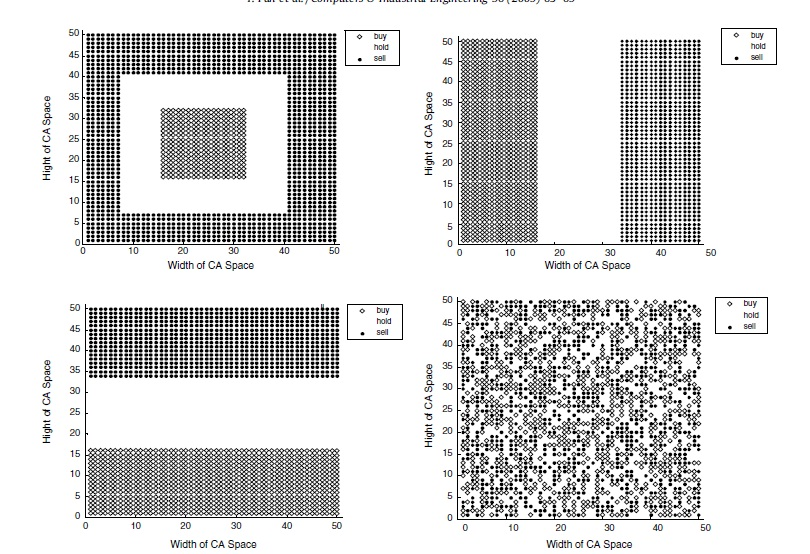
\includegraphics[width=0.8\linewidth]{Figuras/entradas.jpg}
 \caption[Quatro tipos de entrada do estado inicial]{Quatro tipos de entrada do
estado inicial, em (a) quadrado,(b) horizontal, (c)
vertical e (d) aleatório.Retirada de \cite{BaHaKhRa10}} 
\end{figure}
\chapter{Resultados}\label{resultados}

Nessa seção serão apresentados os resultados da simulação e as respectivas
conclusões. Consideramos seis versões diferentes para o teste, cada uma será
explicada devidamente em diferentes sua seções,  baseadas no modelo
descrito na
capítulo \ref{modelo}. Por questão de praticidade vamos representar as versões
pelas seguintes siglas: R, representa rede regular; A, rede aleatória; I,
quantidades dinheiro e ações ilimitadas; e L, limitadas. 

\begin{figure}[!h]
\centering
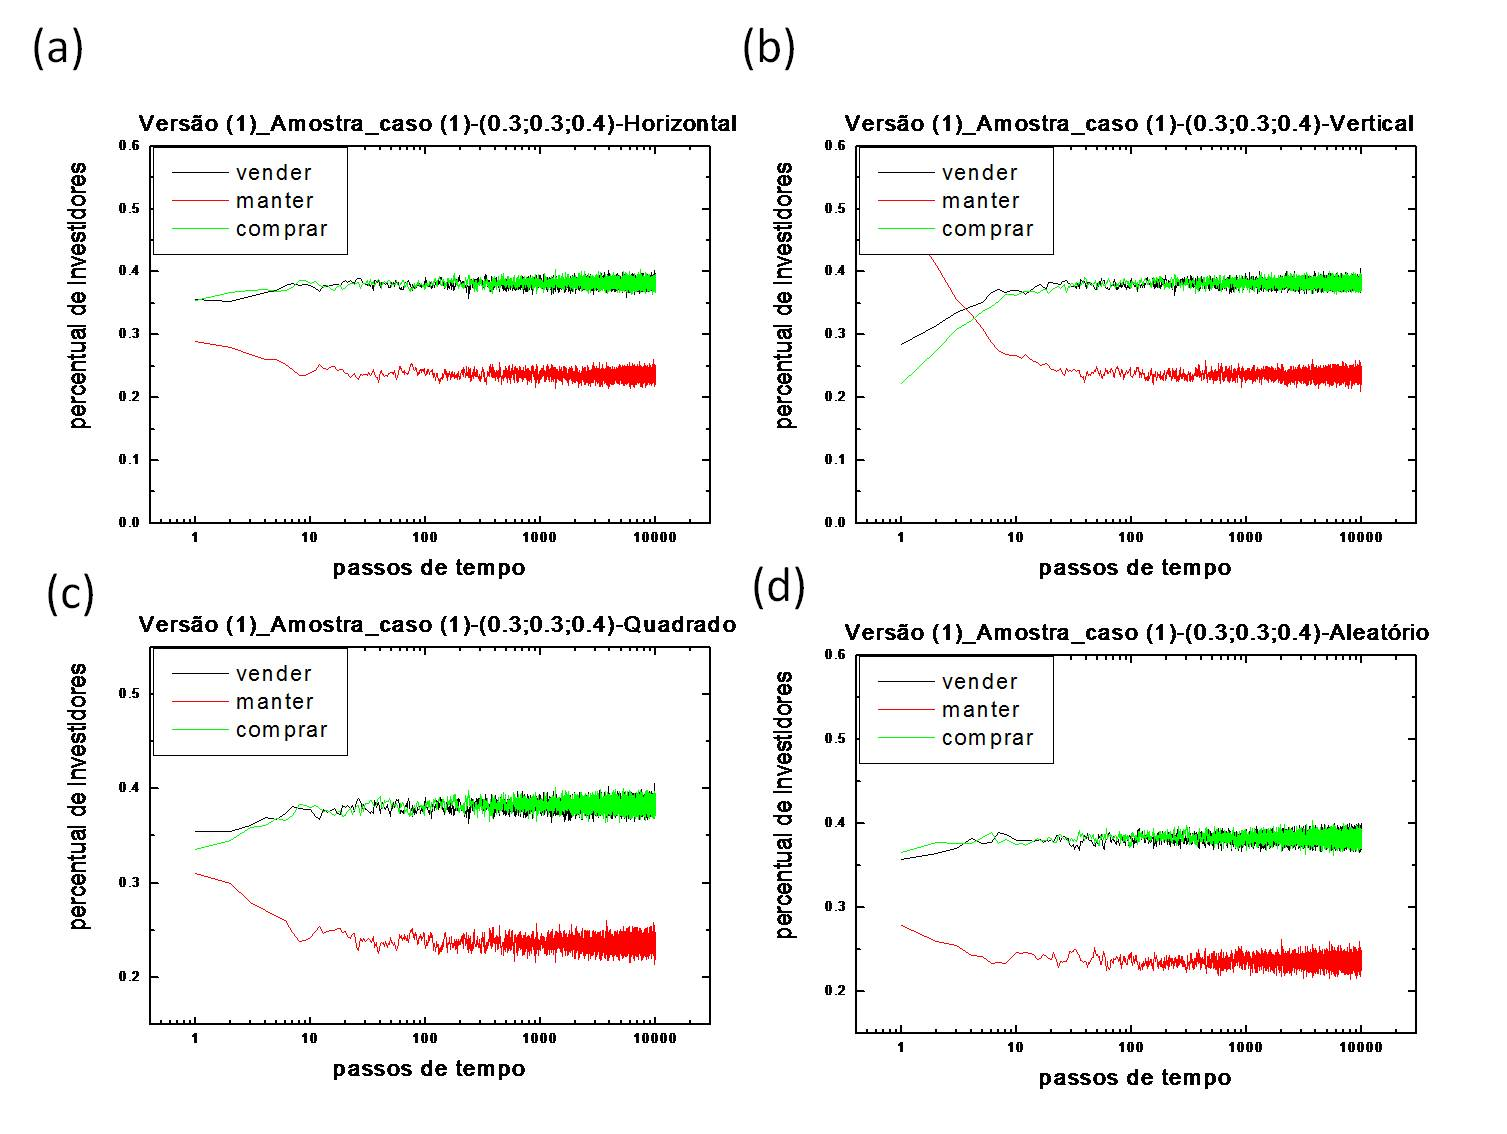
\includegraphics[width=0.8\linewidth]{Figuras/1.jpg}
 \caption[ Evolução do comportamento dos investidores em RI para 4 entradas
diferentes] {Evolução do comportamento dos investidores durante o tempo para
em RIT.3  de uma amostra. Em (a) o estado inicial é
horizontal, em (b) vertical, em (c) listrado e em (d) aleatório com 33\%.
A escala da representação da variação do percentual esta entre 0 e 0.6.}
\label{fig:evolucao-comportamento}
\end{figure}

Na simulação, decidimos variar o percentual de cada tipo de investidores. Assim
variável $P_1(i,j)$ representa a probabilidade de o agente $(i,j)$ ser imitador,
$P_2(i,j)$ representa a probabilidade de o agente $(i,j)$  ser anti-imitador,
$P_3(i,j)= 1-P_2-P_1$ de o agente $(i,j)$ ser indiferente quando o
número de investidores for três e  $P_4(i,j)=1-P_2-P_1-P_3$ do
agente $(i,j)$ ser imitador do mais rico.

Dois conjuntos representados por $(P_1,P_2,P_3)$ e $(P_1,P_2,P_3,P_4)$
foram
simulados pelos seguintes espaços de probabilidade, onde T e Q representam três
 e quatro investidores, respectivamente.

T.1 $P_1(i,j)=P_2(i,j)$ 

T.2 $P_1(i,j)=10P_2(i,j)$ 

T.3 $P_1(i,j)=0.1P_2(i,j)$ 

Q.1 $P_1(i,j)=P_2(i,j)=P_4(i,j)$ 

Q.2 $P_1(i,j)=P_2(i,j)=P_3(i,j)$ 

Q.3 $P_1(i,j)=P_4(i,j)=0.1P_2(i,j)$ 

\begin{figure}[!h]
\centering
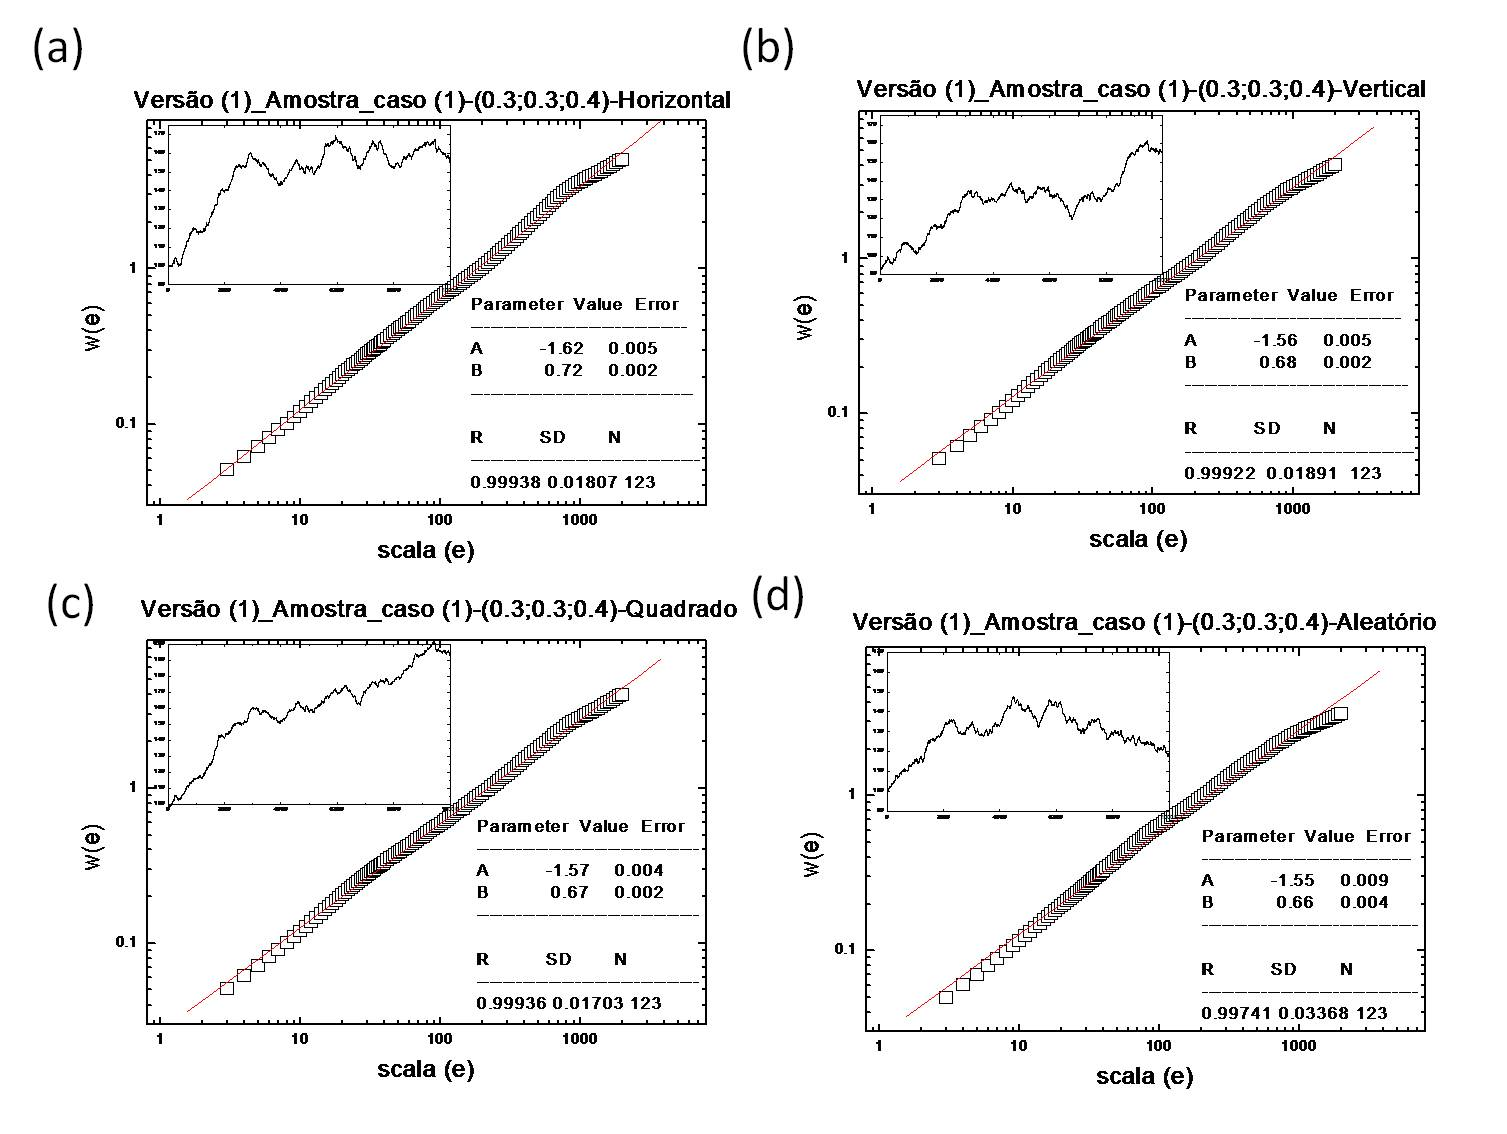
\includegraphics[width=0.8\linewidth]{Figuras/2.jpg}
 \caption[ Cálculo do expoente de Hurst para os índices das ações em RI para 4
entradas diferentes]{Cálculo do expoente de Hurst para os índices das ações de
uma amostra produzidas em RIT.3. O parâmetro B representa o
valor de H. Nos detalhes em cada painel são mostrados os gráficos do índice
das ações. Em (a) o estado inicial é horizontal, em (b) vertical, em (c)
listrado e em (d) aleatório com 33\%.}
\label{fig:expoente-hurst}
\end{figure}

Representaremos, por exemplo, RIT.2 a versão referente a rede
regular e a quantidade de dinheiro e ações ilimitadas.  Testamos os quatro casos
iniciais, representados nas figuras
\ref{fig:evolucao-comportamento} e \ref{fig:expoente-hurst}, horizontal,
vertical, aleatório e listrado no caso (0.3;0.3;0.4), escolhida aleatoriamente,
observamos que a tendência é a mesma. Assim, decidimos fazer todas as simulações
pelo estado inicial considerando-se uma distribuição aleatória: em que a opção
inicial de cada investidor é sorteada aleatoriamente com probabilidade de 1/3
para cada ação (comprar, vender, manter).

\begin{figure}[!h]
\centering
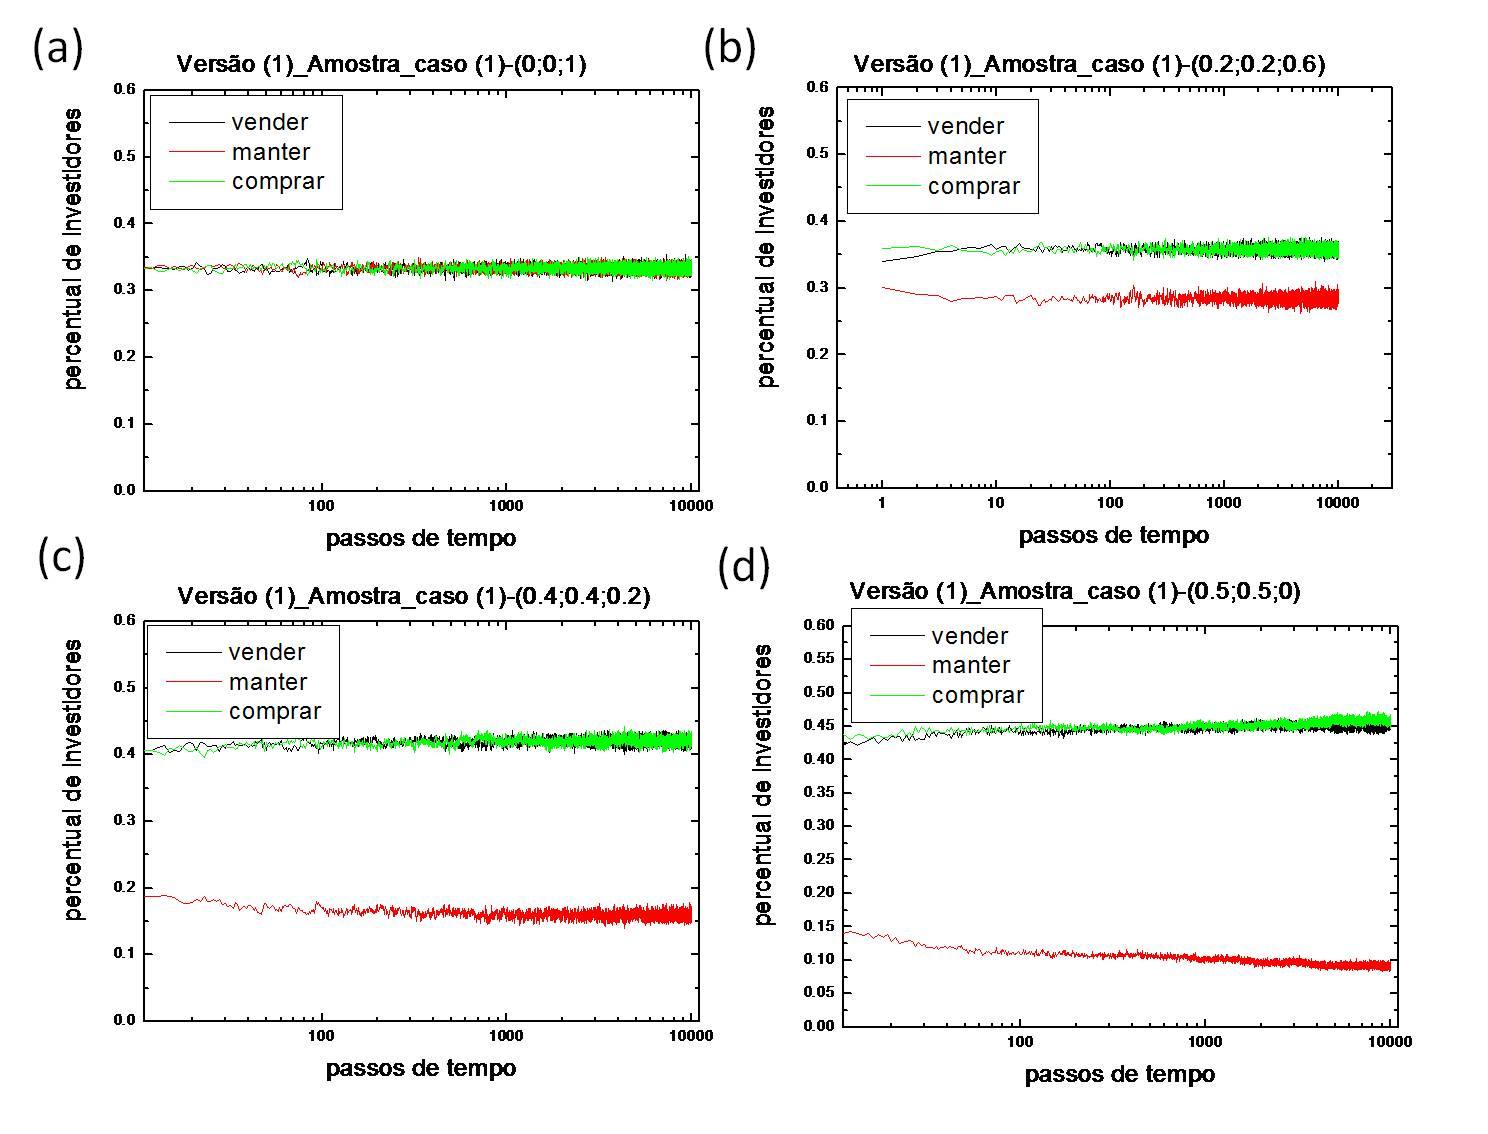
\includegraphics[width=0.8\linewidth]{Figuras/3.jpg}
 \caption [Evolução do comportamento dos investidores em RIT.1]{Evolução do
comportamento dos investidores durante o tempo em RIT.1 de uma amostra. }
\label{fig:evolucao-comp-investidores}
\end{figure}

\begin{figure}[!h]
\centering
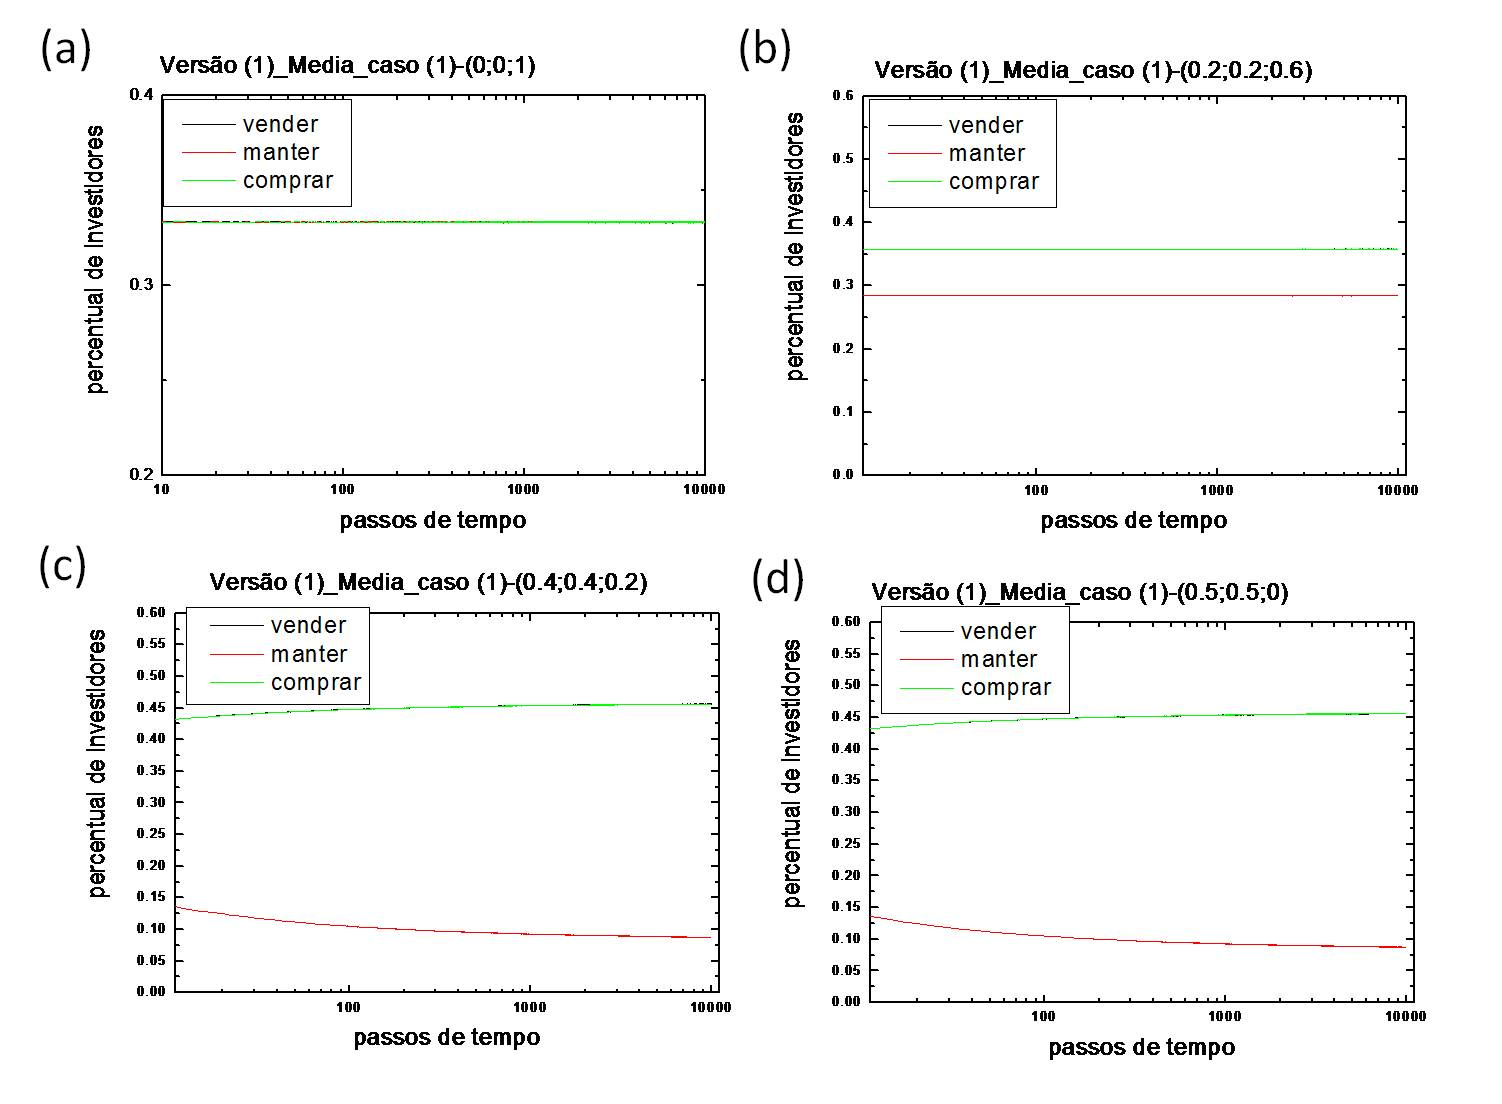
\includegraphics[width=0.8\linewidth]{Figuras/4.jpg}
\caption [Evolução média do comportamento dos investidores em RIT.1]{Evolução do
comportamento dos investidores durante o tempo para a média
das 1000 amostras em em RIT.1 .}
\label{fig:evolucao-comp-investidores2}
\end{figure}

\begin{figure}[!h]
\centering
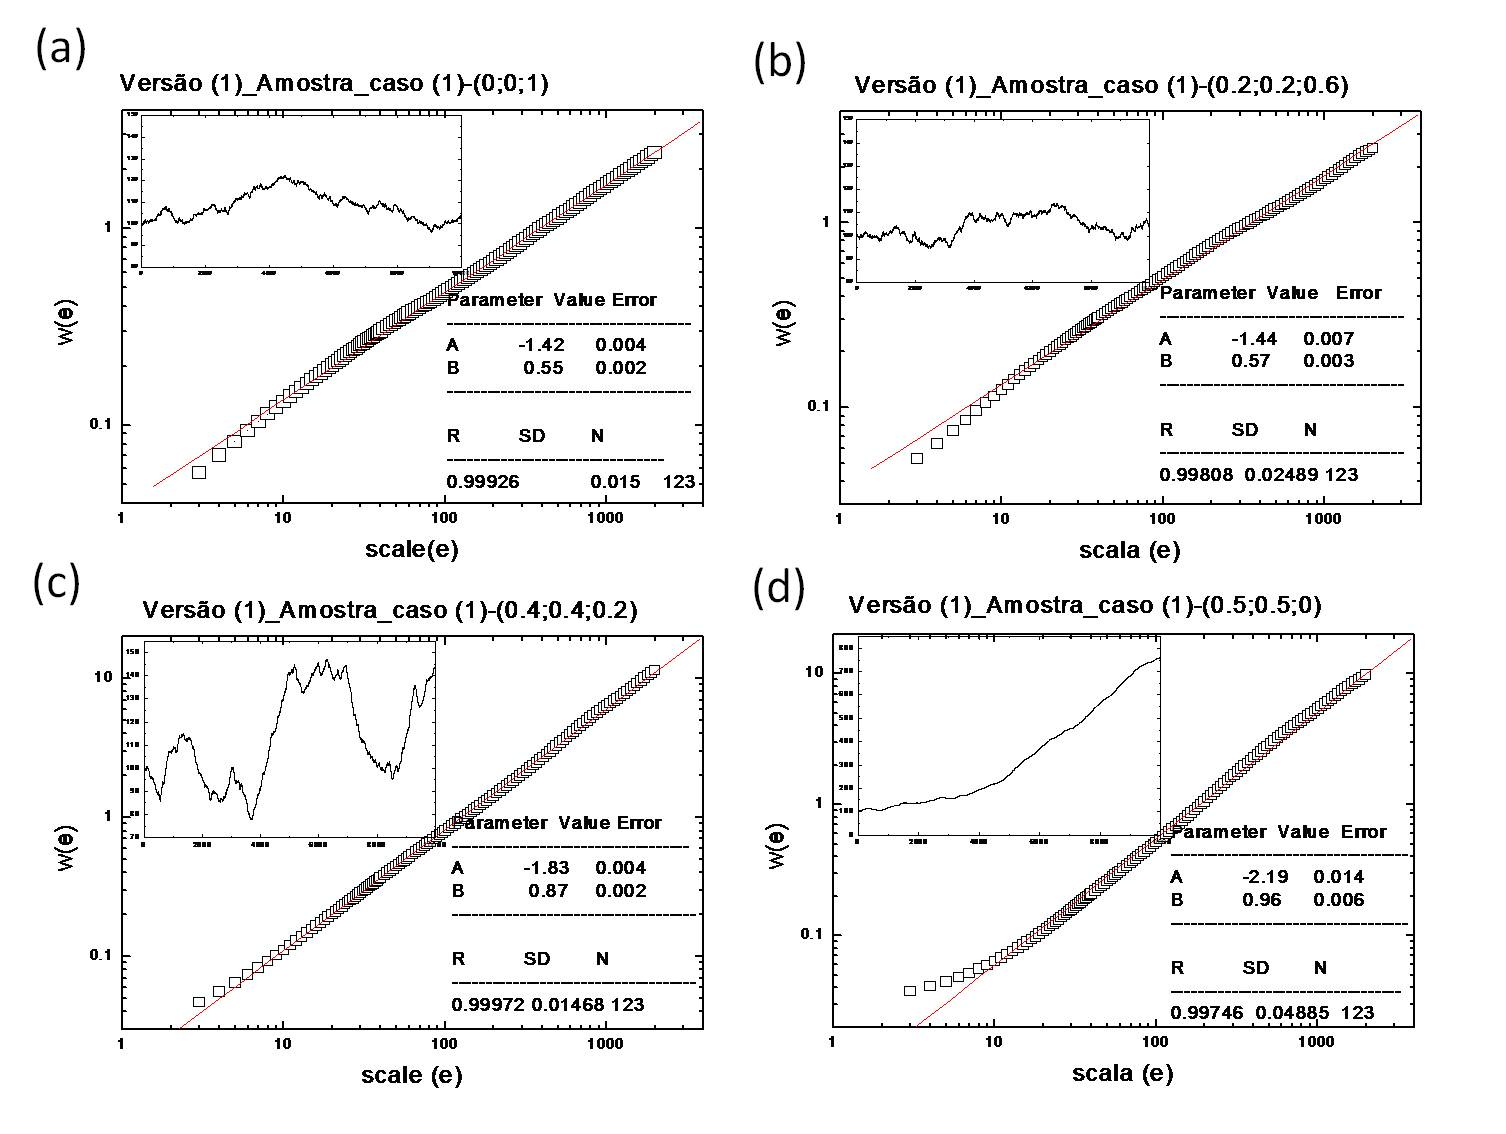
\includegraphics[width=0.8\linewidth]{Figuras/5.jpg}
 \caption [Cálculo do expoente de Hurst para os índices das ações em RIT.1]
{Cálculo do expoente de Hurst para os índices das ações de uma amostra
produzidas em RIT.1. O parâmetro B representa o valor de H. Nos
detalhes em cada painel são mostrados os gráficos do índice das ações. Na
maioria dos casos representamos os índices variando de 80 a 150, em (d) o
índice chegou a 800.}
\label{fig:calculo-expoente-hurst}
\end{figure}

Para cada um dos casos, foram simuladas 1.000 amostras, durante 10.000 passos
de tempo. O tempo computacional foi aproximadamente de um dia e três dias, para
as versões com rede regular e rede aleatória, respectivamente.  Comparando-se os
resultados do caso médio das 1.000 amostras com 1 amostra, em RIT.1 que
será explicada sub-seção seguinte, observa-se em todos os casos  a  mesma
tendência, ou seja, os resultados apresentados referentes a média são
semelhantes ao da amostra. Como exemplificado nas figuras
\ref{fig:evolucao-comp-investidores}; \ref{fig:evolucao-comp-investidores2};
\ref{fig:calculo-expoente-hurst} e \ref{fig:calculo-expoente-hurst2}.
Assim, por esse motivo vamos representar a evolução do comportamento dos
investidores e o gráfico do cálculo do expoente de Hurst e o índice pelos
gráficos de uma amostra. Já o valor do expoente de Hurst será apresentado ao
final de cada sub-seção referente a média das 1000 amostras. 


\begin{figure}[!h]
\centering
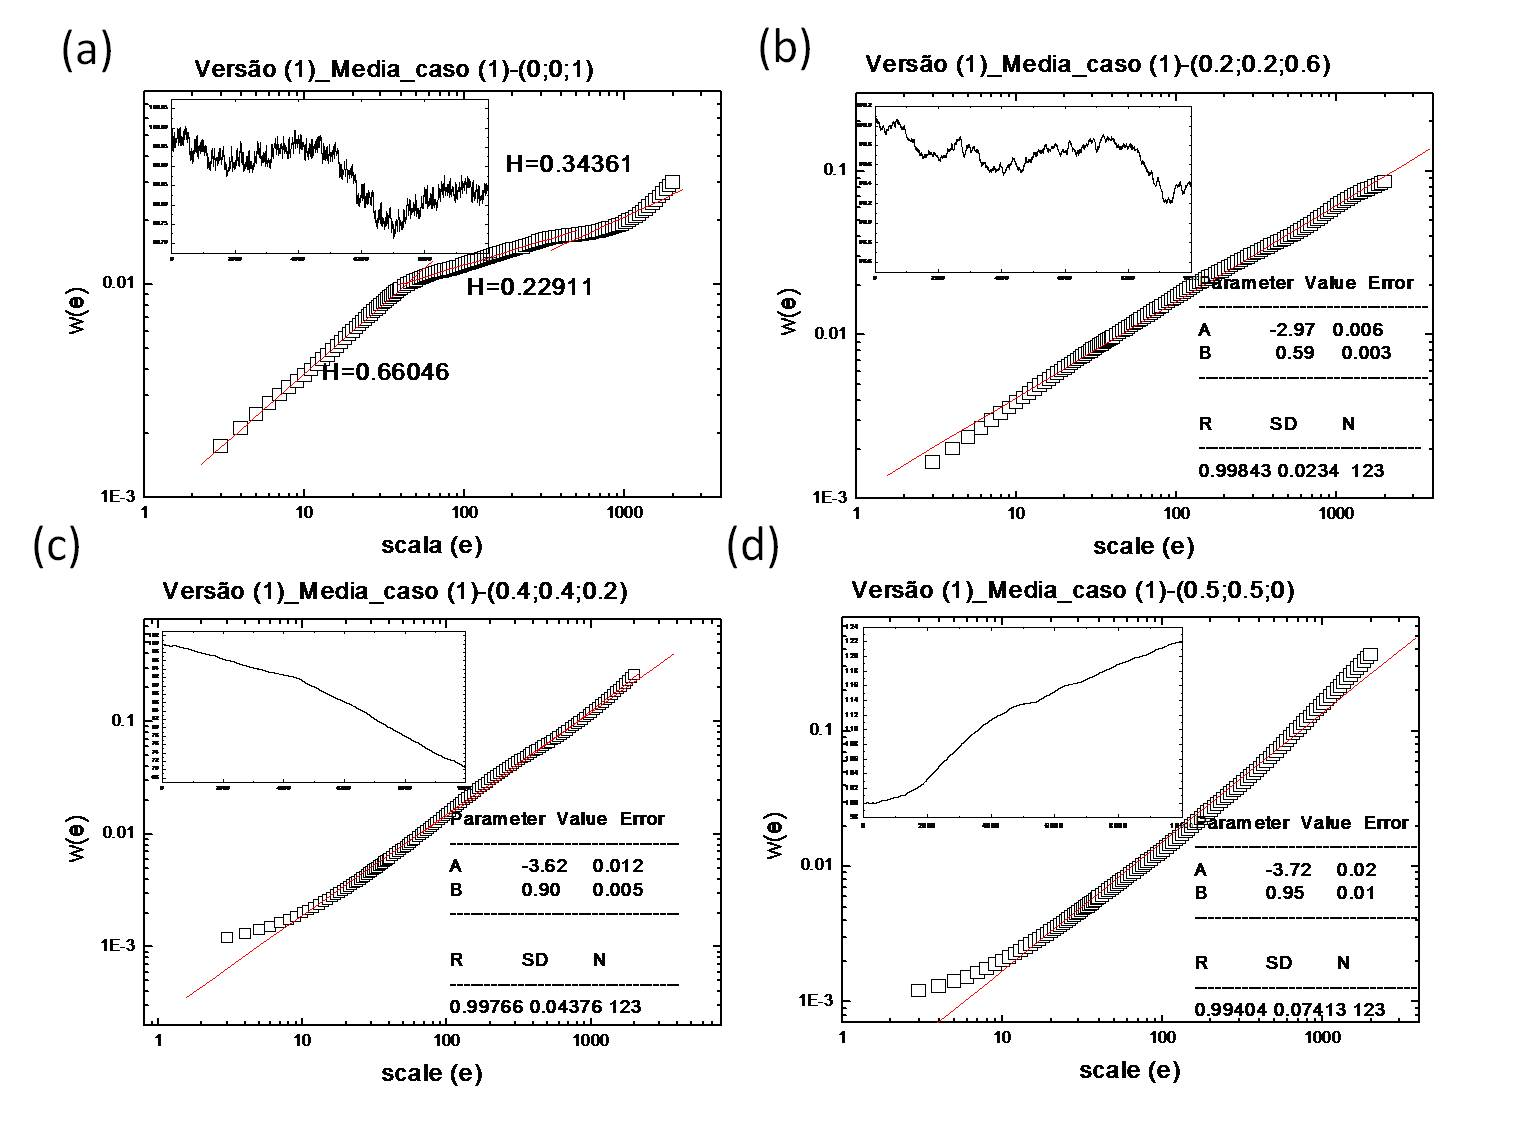
\includegraphics[width=0.8\linewidth]{Figuras/6.jpg}
\caption [Cálculo do expoente de Hurst para os índices médio das ações em
RIT.1]{Cálculo do expoente de Hurst para os índices médio das ações referente
a 1000 amostras produzidas no caso (1) na versão (1). O parâmetro B representa
o valor de H. Nos detalhes em cada painel são mostrados os gráficos do índice
das ações. Em (a) e (b) representamos os índices variando de aproximadamente
98,6 a 100, 2, em (c) de 68 a 102 e (d) de 100 a 124.}
\label{fig:calculo-expoente-hurst2}
\end{figure}

\section{ RIT}

Nessa primeira versão, a RIT, a rede é regular e a quantidade de dinheiro e
ações é infinita. Considerou-se três tipos de comportamento para os
investidores. O ''imitador'', o ''anti-imitador'' e o “indiferente”, os
casos  T.1, T.2 e T.3. 

Em todos os casos, observa-se, como esperado, que o número de investidores
em cada uma das escolhas flutua aleatoriamente e o índice de ações refletem
esse comportamento, exibindo características auto-similares.

\begin{figure}[!h]
\centering
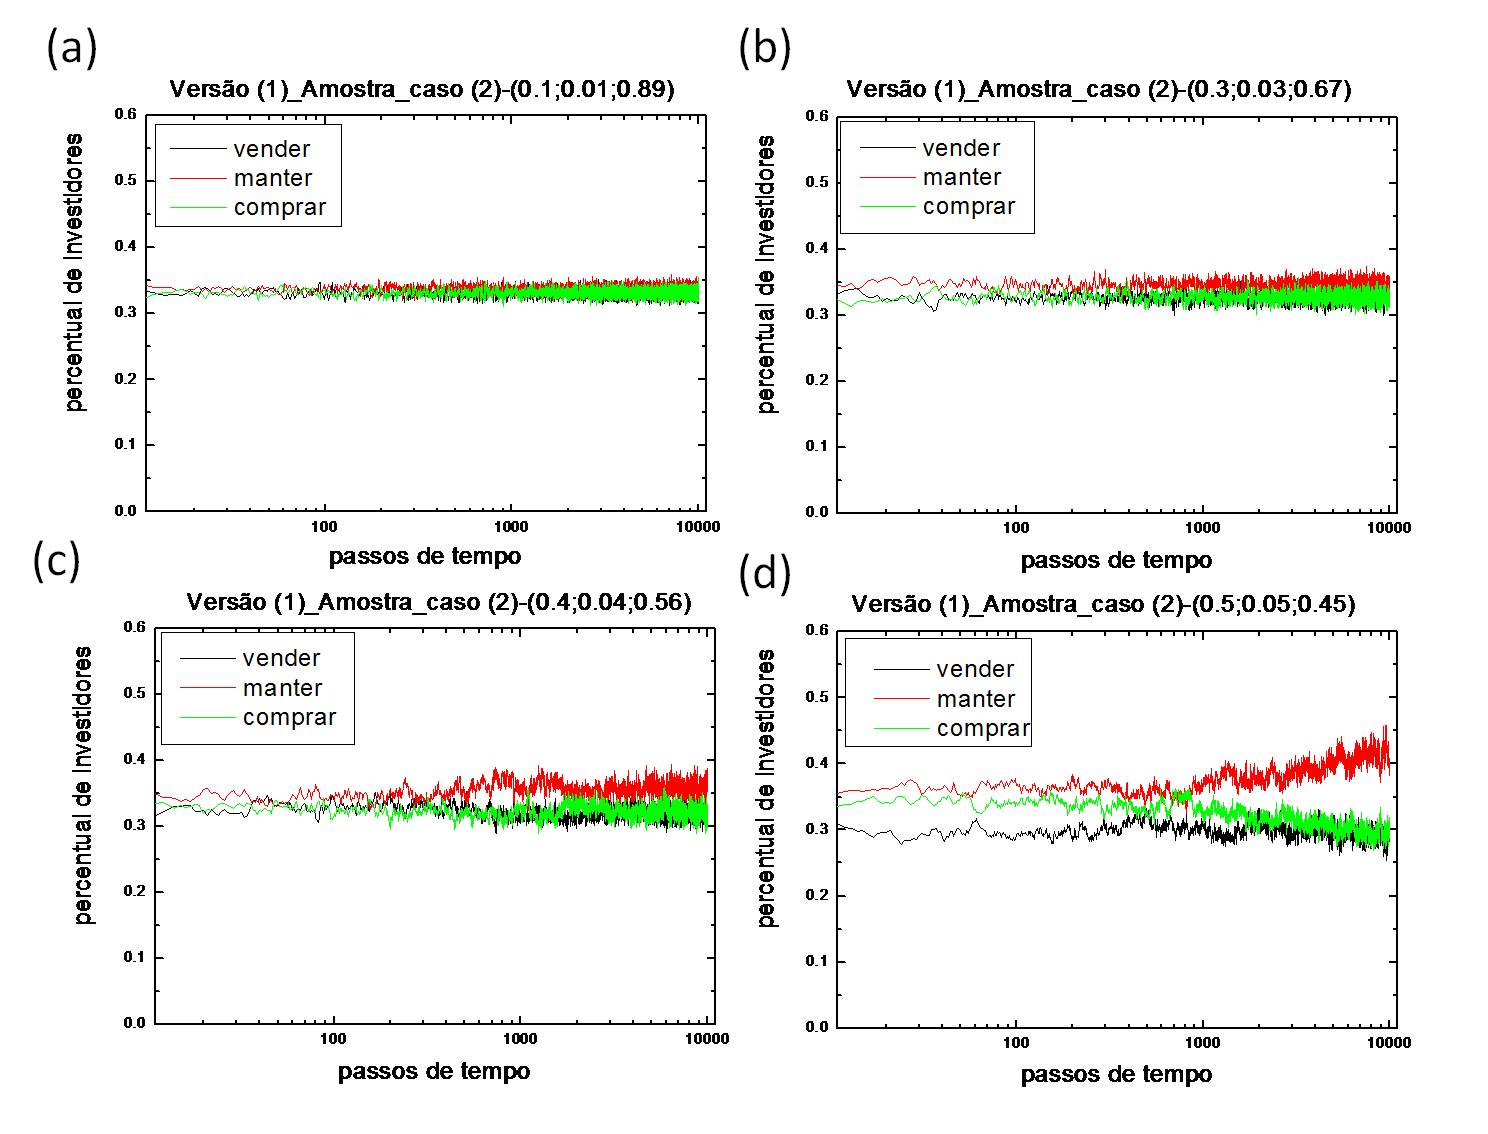
\includegraphics[width=0.8\linewidth]{Figuras/7.jpg}
 \caption[Evolução do comportamento dos investidores em RIT.2]{Evolução do
comportamento dos investidores durante o tempo para caso
em RIT.2 }
\label{fig:evolucao-comportamento2}
\end{figure}

Em RIC.1, verifica-se que o número de pessoas que está vendendo e comprando
geralmente é proporcional, e à medida que $P_1$ e $P_2$ aumentam, o número de
pessoas que está mantendo diminui, como observado na figura
\ref{fig:evolucao-comp-investidores}.  Esse aumento de $P_1$ e $P_2$ influencia
diretamente os preços do mercado, causando enormes flutuações, como observado
nas figuras 5.5 (c) e 5.5 (d). Já no caso em que $P_1$ e $P_2$, o
índice do mercado varia pouco, como em 5.5 (a) e 5.5 (b).

\begin{figure}[!h]
\centering
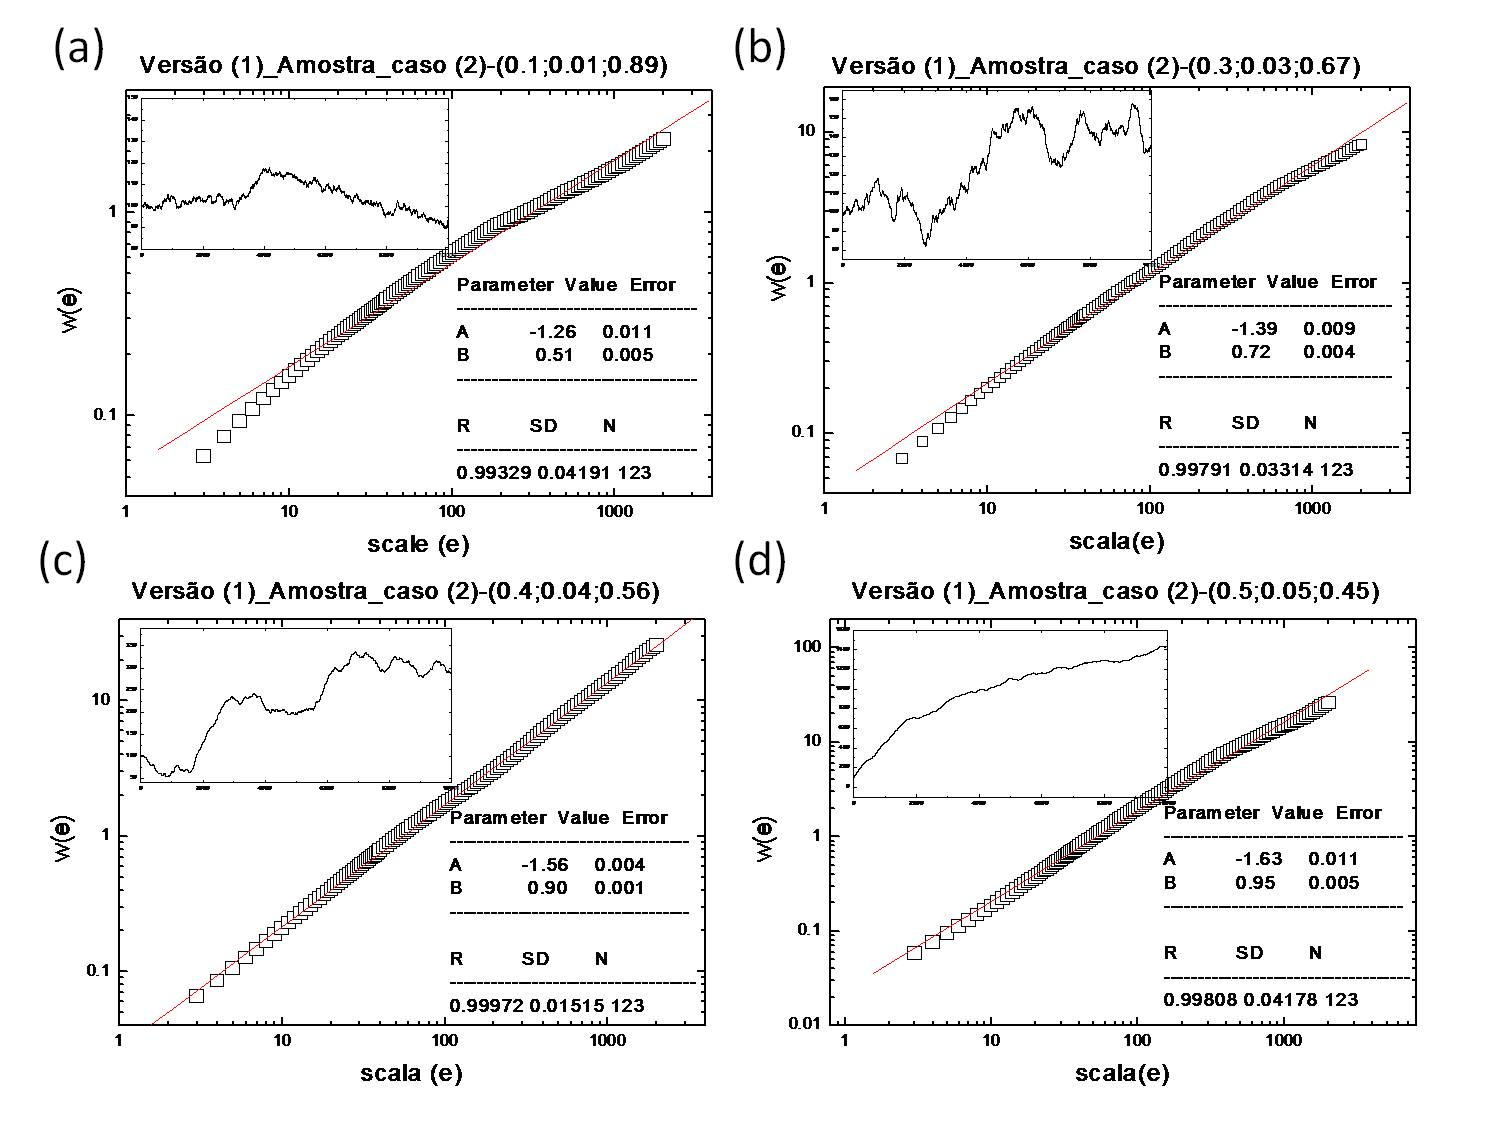
\includegraphics[width=0.8\linewidth]{Figuras/8.jpg}
 \caption[ Cálculo do expoente de Hurst para os índices em RIT.2] {Cálculo do
expoente de Hurst para os índices de uma amostra produzida em RIT.2.  O
parâmetro B representa o valor de H. Nos detalhes em cada painel são mostrados
os gráficos do índice das ações.}
\label{fig:calculo-expoente-hurst3}
\end{figure}

Em RIT.2, tem-se que, à medida que $P_1$ aumenta, o efeito manada é
acentuado,
como observado na figura \ref{fig:evolucao-comportamento2}, principalmente em
\ref{fig:evolucao-comportamento2} (d). Esta característica
também influencia o aumento das flutuações no mercado, principalmente em
\ref{fig:calculo-expoente-hurst3}(b), \ref{fig:calculo-expoente-hurst3}(c) e
\ref{fig:calculo-expoente-hurst3}(d). Já em
\ref{fig:calculo-expoente-hurst3}(d), o índice chega 1600 no final da
simulação, ou seja, um aumento de 16 vezes o valor inicial.

\begin{figure}[!h]
\centering
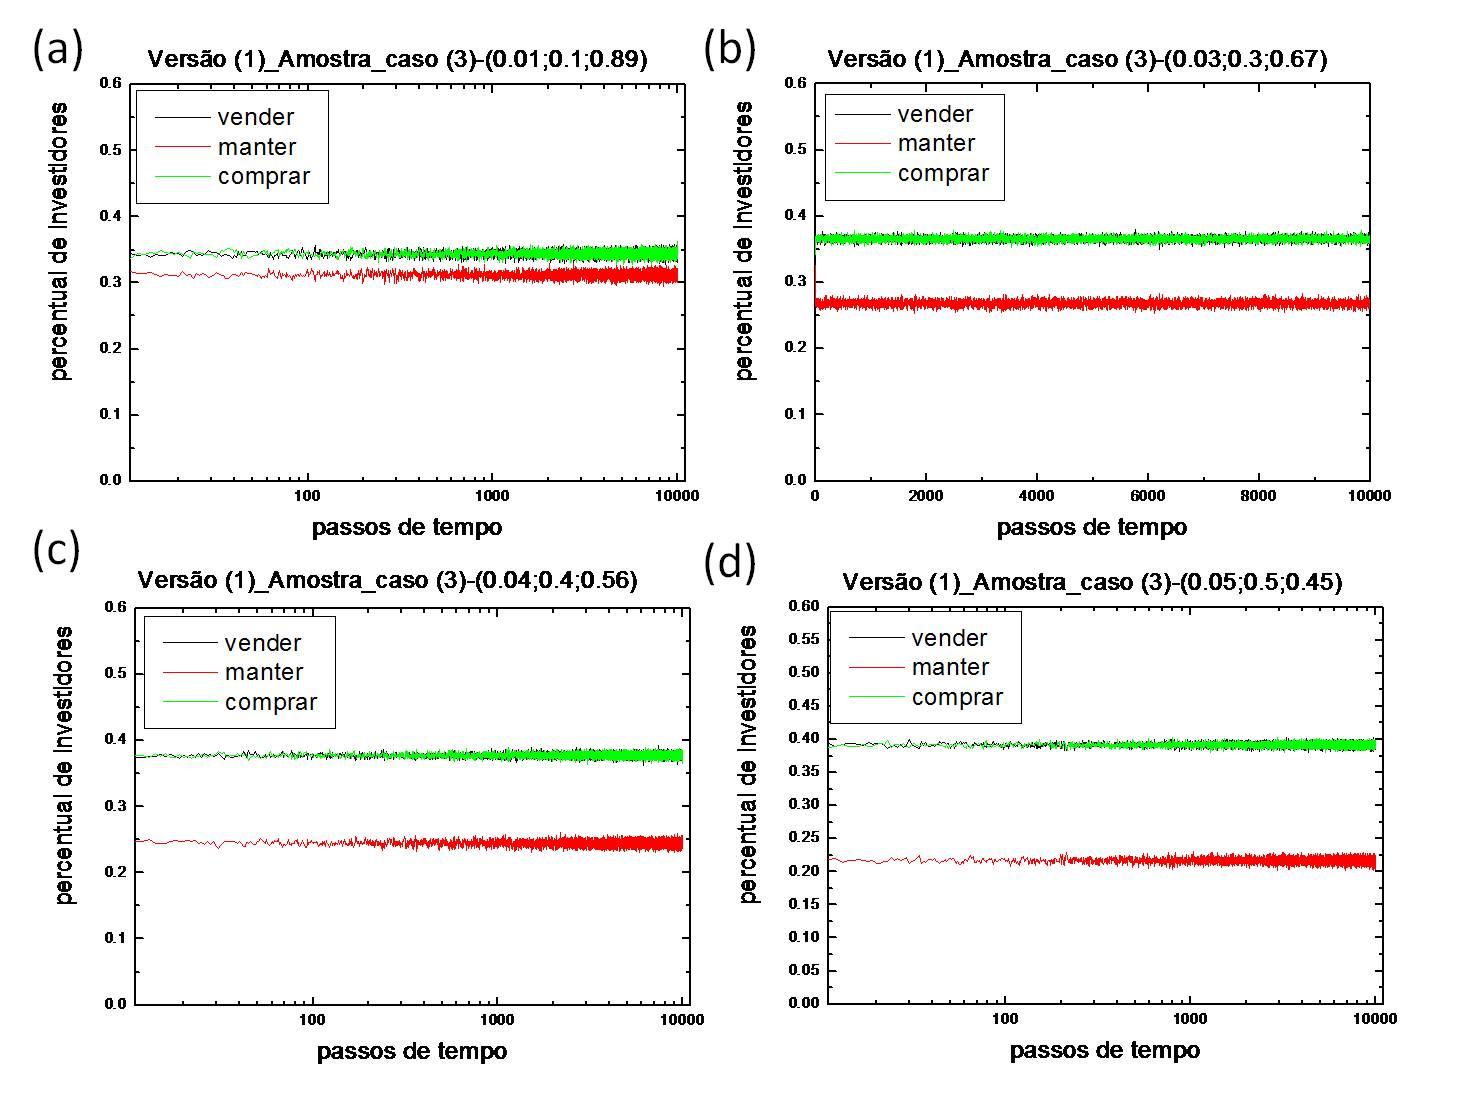
\includegraphics[width=0.8\linewidth]{Figuras/9.jpg}
\caption [Evolução do comportamento dos investidores em RIT.3.]{Evolução do
comportamento dos investidores durante o tempo em RIT.3 de uma amostra.}
\label{fig:evolucao-comportamento3}
\end{figure}

Em RIT.3, observamos que, o número de pessoas que está vendendo e comprando
geralmente é proporcional, e à medida que $P_2$ aumenta, o número de pessoas que
está mantendo diminui, como observado na
figura \ref{fig:evolucao-comportamento3}.  Com o aumento do número de
investidores independentes P3 e diminuindo o número de investidores imitadores
$P_1$, o mercando varia pouco, mantendo estável em todas as situações, como
exemplificado na figura \ref{fig:calculo-expoente-hurst4}.

\begin{figure}[!h]
\centering
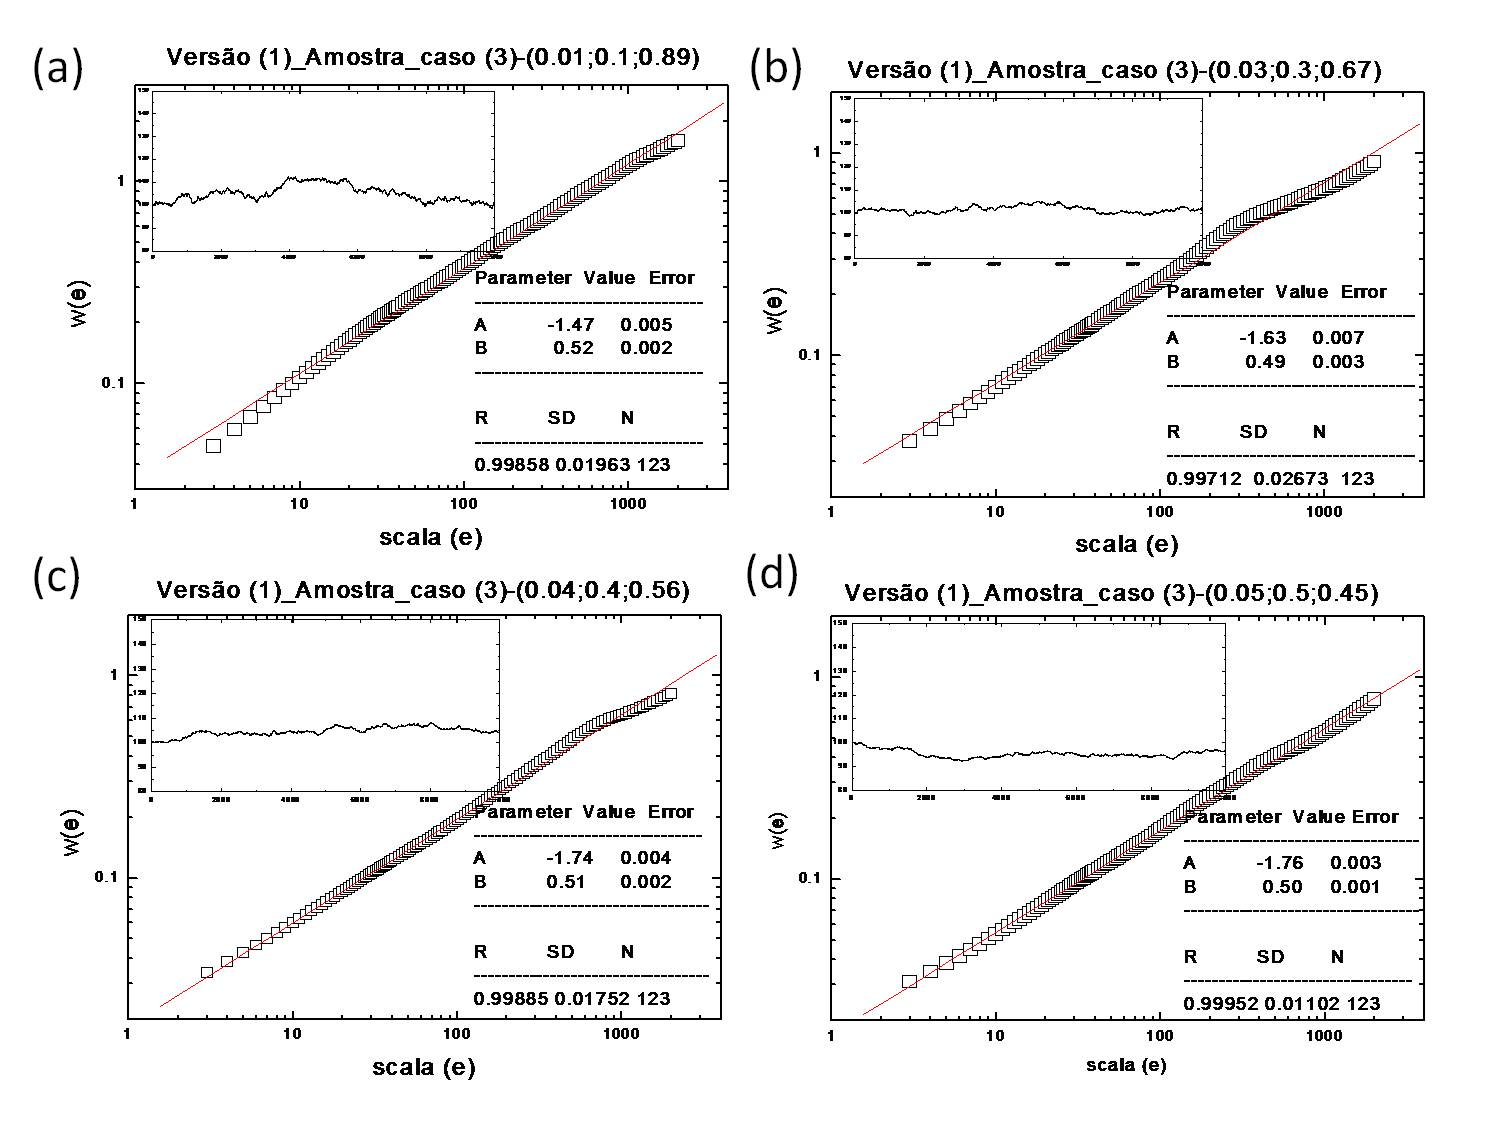
\includegraphics[width=0.8\linewidth]{Figuras/10.jpg}
\caption[ Cálculo do expoente de Hurst para os índices em RIT.3] {Cálculo do
expoente de Hurst para os índices de uma amostra produzida em RIT.3.  O
parâmetro B representa o valor de H. Nos detalhes em cada painel são mostrados
os gráficos do índice das ações. }
\label{fig:calculo-expoente-hurst4}
\end{figure}

\begin{figure}[!h]
\centering
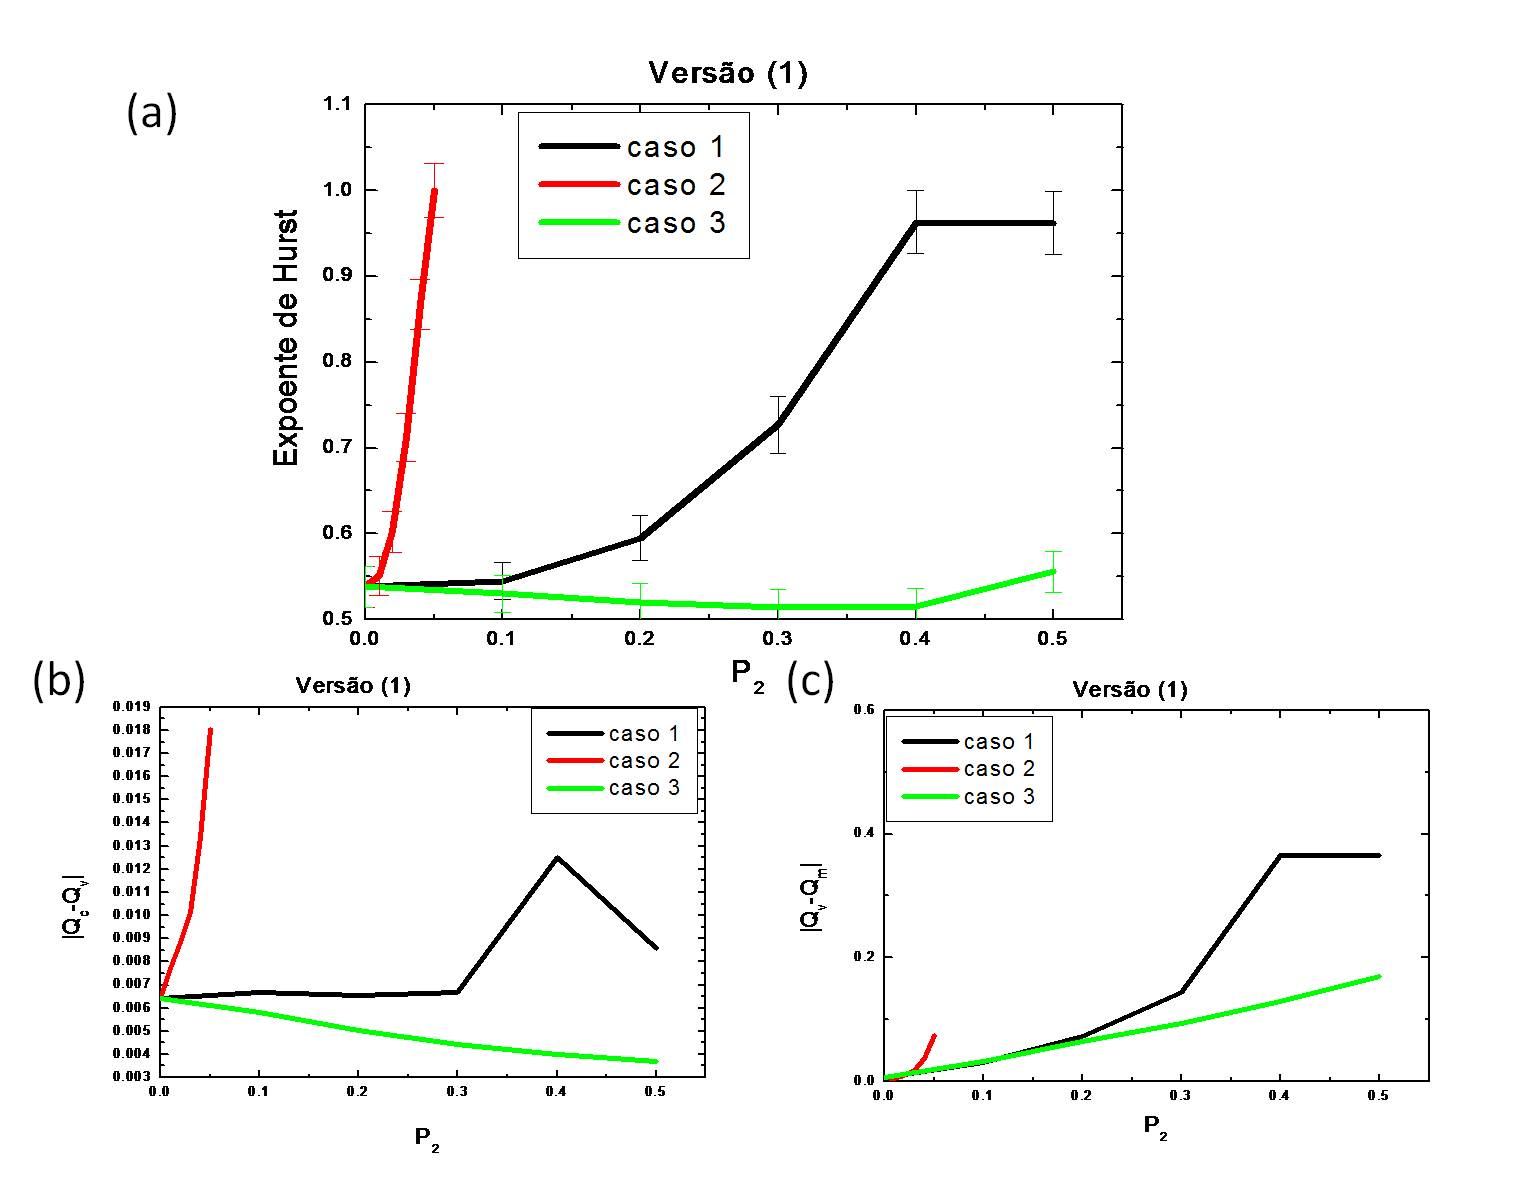
\includegraphics[width=0.8\linewidth]{Figuras/11.jpg}
\caption[Análise do expoente de Hurst em RIT]{Na figura 5.11.a é representado no
gráfico o valor médio das 1000 amostras do expoente de Hurst em RIT para cada
caso em função de $P_2$.
Na figura \ref{fig:valor-medio}(b) é representada a porcentagem da diferença
entre o número de pessoas que estão comprando ($Q_b$) e as que estão vendendo
($Q_s$) (cálculo do efeito médio de manada para os estados comprar ou vender)
em função de $P_2$. Na figura \ref{fig:valor-medio}(c) é representada da
diferença entre o número de pessoas que estão no estado comprar ($Q_b$) e as que
estão estado vender ($Q_h$) (que é igual à diferença entre o número pessoas que
estão
vendendo e as que estão mantendo) em função de $P_2$, ou seja, é calculada a
porcentagem da diminuição da escolha ``manter''.}
\label{fig:valor-medio}
\end{figure}


Na figura 5.11, observamos que em RIT.1 e RIT.2, o efeito de ``manada'',
influencia diretamente no valor do expoente de Hurst, principalmente o RIC.2, em
que seus valores são maiores.  Já em RIT.3, a diminuição do efeito “manada”, até
um certo valor de $P_2$, influencia na diminuição do expoente de Hurst. Mas à
medida que a diminuição do  estado “manter” aumenta, o expoente de Hurst também
aumenta. Ou seja, o efeito manada e a diminuição da estado manter, influenciam
diretamente o valor do expoente de Hurst, sendo que o efeito manada apresenta
uma maior influencia. 
   
Em RIT.1, fica claro que o aumento de $P_1$ (investidores imitadores)
aumenta a tendência para $H>0,5$, que rapidamente fica parecido com os dos
mercados de países emergentes. 

Em RIT.2, em que a porcentagem de investidores imitadores é 10 vezes
maior que a de investidores anti-imitadores, o efeito de manada aumenta à medida
que $P_1$ aumenta, mais rapidamente que nos outros casos, relação que já foi
observada na figura 3. Desse modo $H$ é maior do que os outros
casos, e , converje mais rápido.	

Em RIT.3, em que o número de anti-imitadores é
10 vezes maior que o número de imitadores e o número de indiferentes varia de
acordo com o número de anti-imitadores (quanto menor o número de
anti-imitadores, maior o número de indiferentes), observamos a tendência de
$H\sim (1/2)$, o que é esperado para um mercado eficiente. Mesmo com o aumento
de
$P_2$, e com a diminuição do número de investidores que estão na estado manter,
o expoente hurst varia pouco.





\begin{figure}[!h]
\centering
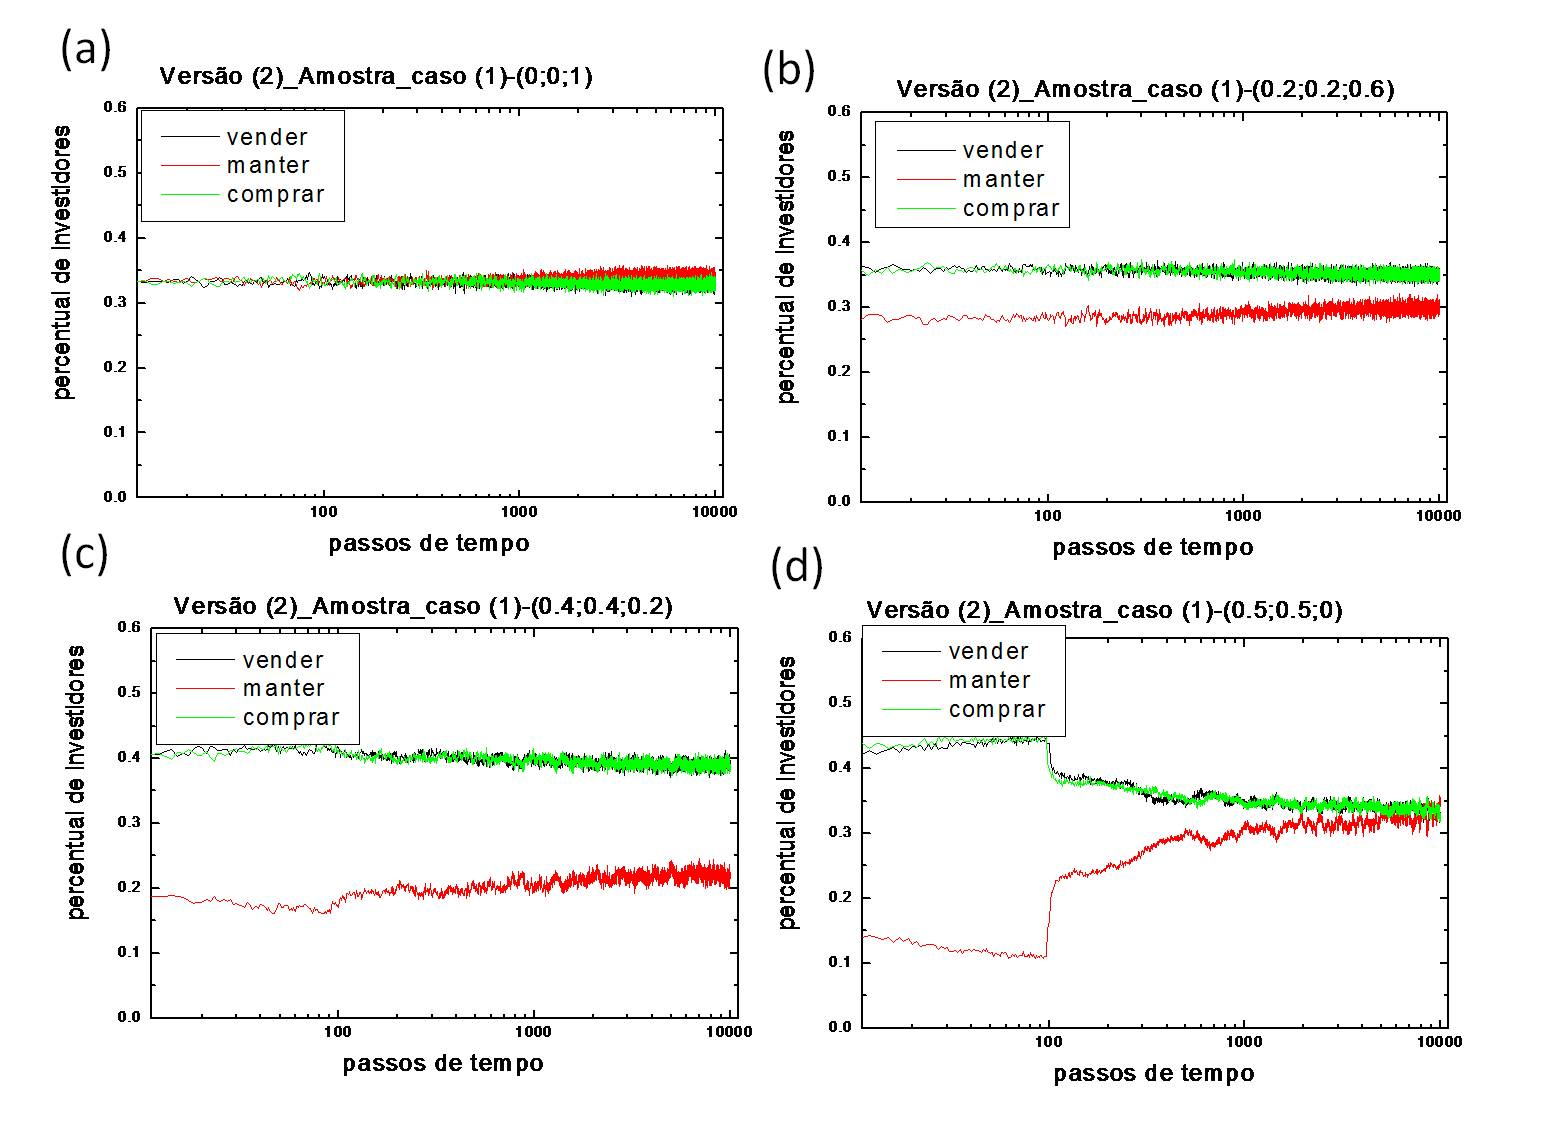
\includegraphics[width=0.8\linewidth]{Figuras/12.jpg}
\caption [Evolução do comportamento dos investidores em RLT.1]{Evolução do
comportamento dos investidores durante o tempo em RLT.1 de uma amostra. }
\label{fig:evolucao-comportamento4}
\end{figure}

\section{RLT}

Na simulação da versão (2), a RLT, os parâmetros são quase todos os mesmos,
exceto em que as quantidades de dinheiro e ações iniciais são limitadas, sendo
seus
valores iniciais, 10000 e 100, respectivamente.  Como consequência, regras foram
criadas como descritas no capítulo \ref{modelo}.

\begin{figure}[!h]
\centering
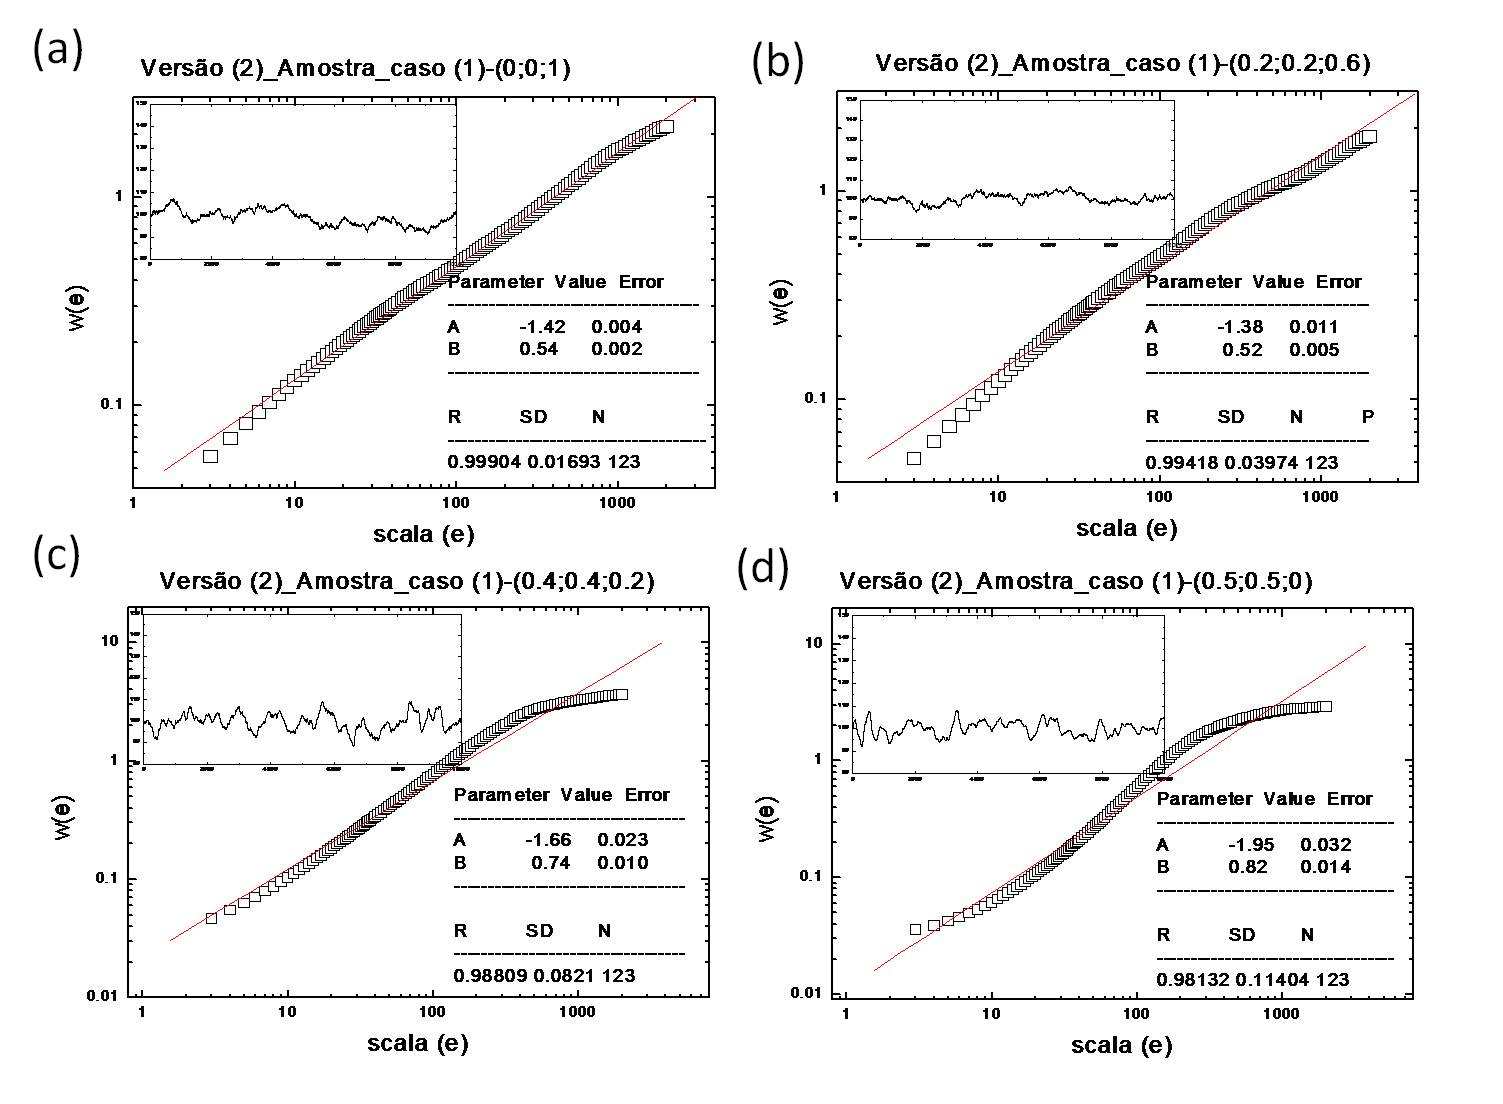
\includegraphics[width=0.8\linewidth]{Figuras/13.jpg}
\caption[ Cálculo do expoente de Hurst para os índices em RLT.1] {Cálculo do
expoente de Hurst para os índices de uma amostra produzida em RLT.1.  O
parâmetro B representa
o valor de H. Nos detalhes em cada painel são mostrados os gráficos do índice
das ações. O índice esta representado variando de 80 a 150.}
\label{fig:calculo-expoente-hurst5}
\end{figure}

Em RLT.1, à medida que  $P_1$ e $P_2$ aumentam, o número de
pessoas que estão mantendo tende a aumentar mais ao longo do tempo comparado ao
RIT.1, significando que tomaram essa atitude por falta de
dinheiro ou ações, como exemplificado na figura
\ref{fig:evolucao-comportamento4}. Essa limitação faz com que as flutuações do
mercado sejam menores, comparada ao RIT.1, como ilustrado na
figura \ref{fig:calculo-expoente-hurst5}.

\begin{figure}[!h]
\centering
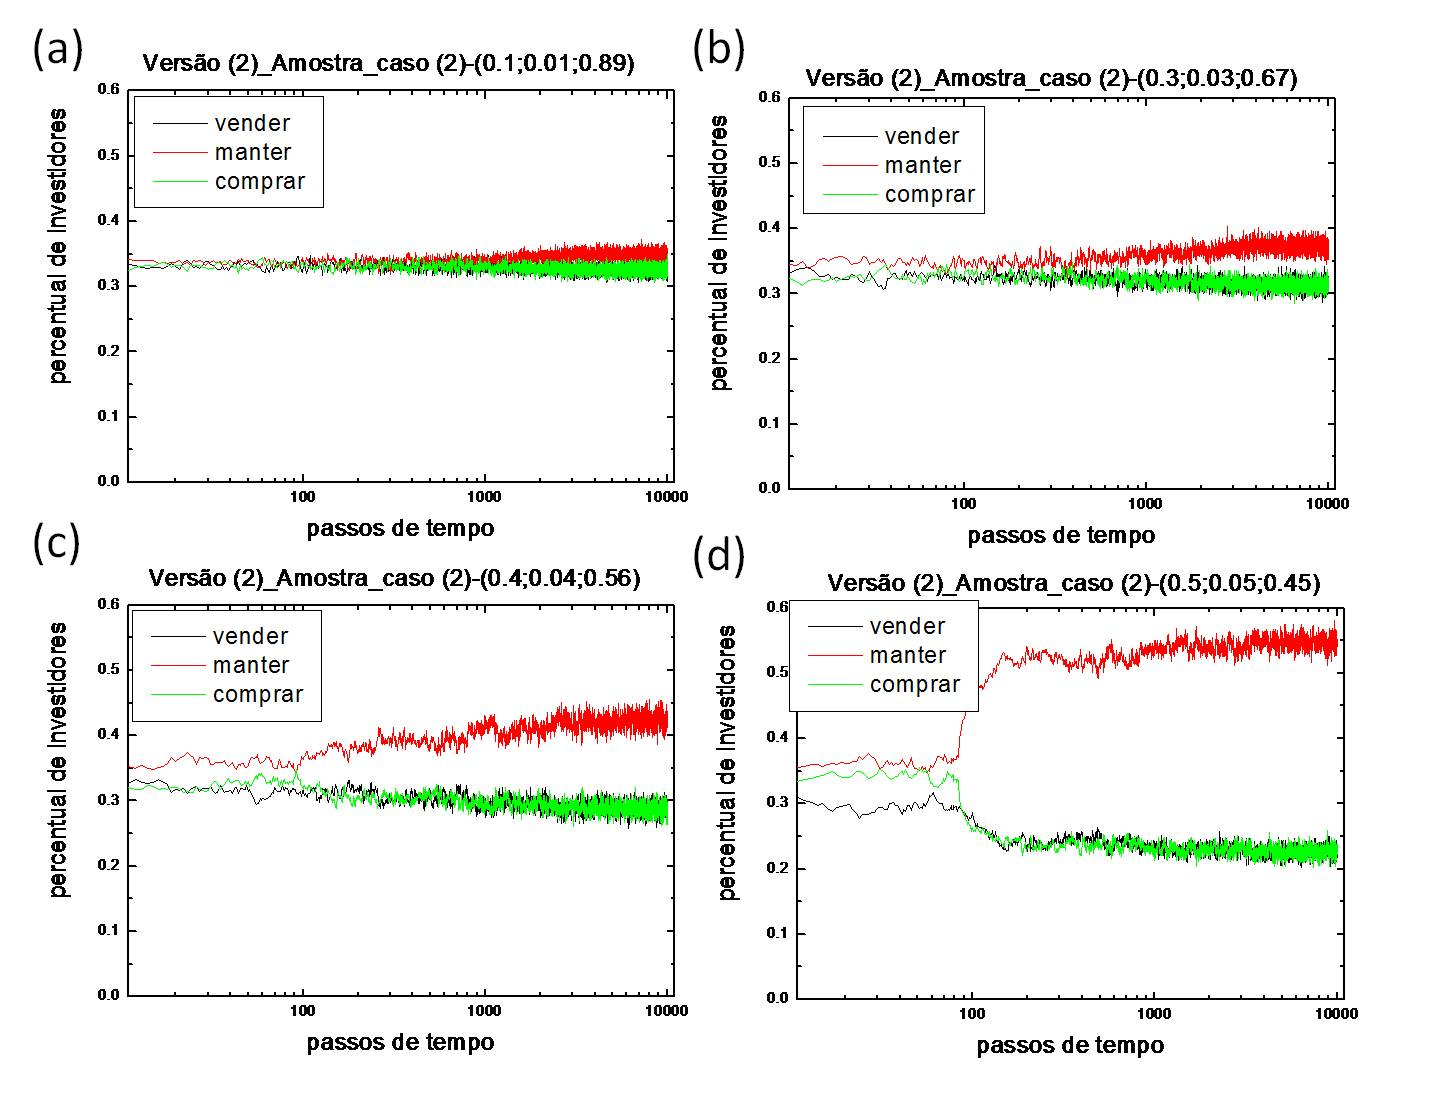
\includegraphics[width=0.8\linewidth]{Figuras/14.jpg}
\caption[Evolução do comportamento dos investidores em RLT.2]{Evolução do
comportamento dos investidores durante o tempo em RLT.2.}
\label{fig:evolucao-comportamento5}
\end{figure}

\begin{figure}[!h]
\centering
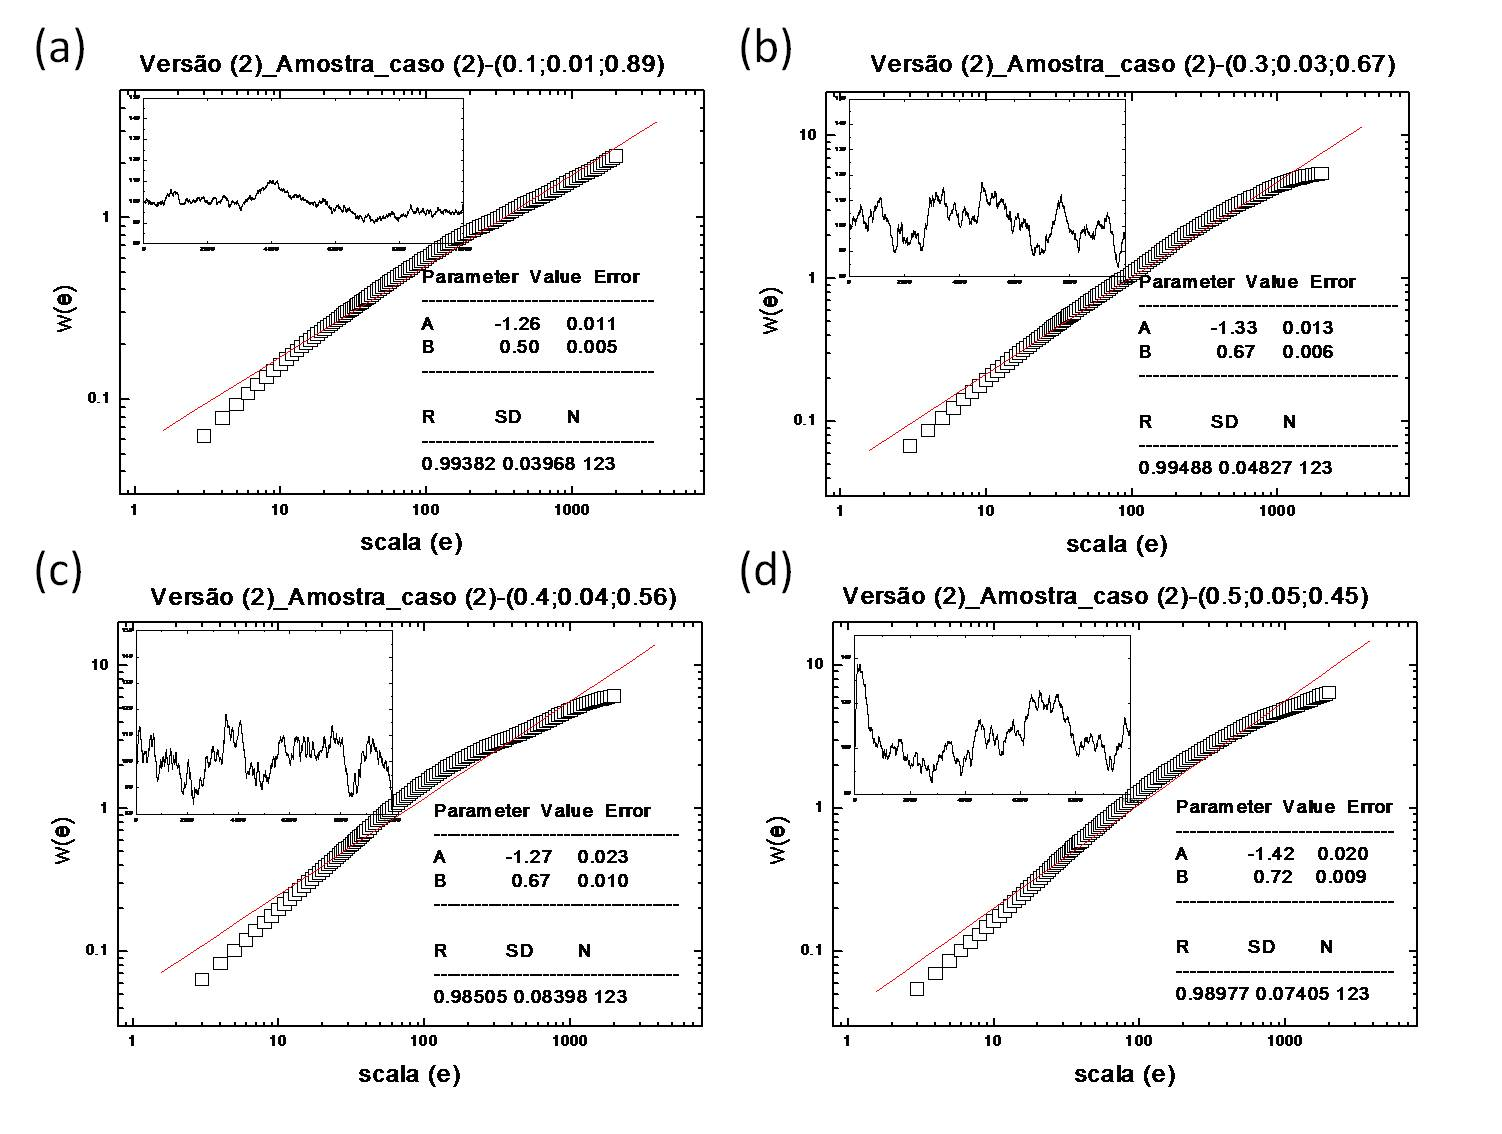
\includegraphics[width=0.8\linewidth]{Figuras/15.jpg}
\caption[ Cálculo do expoente de Hurst para os índices em RLT.2] {Cálculo do
expoente de Hurst para os índices de uma amostra produzida em RLT.2.  O
parâmetro B representa o valor de H. Nos detalhes em cada painel são mostrados
os gráficos do índice
das ações.  }
\label{fig:calculo-expoente-hurst6}
\end{figure}

Analisando a figura \ref{fig:evolucao-comportamento5}, observamos que em RLT.2,
à medida que $P_1$ aumenta o número de pessoas que estão na escolha manter
aumenta mais rápido que em RIT.2. Significando que várias pessoas, em algum
passo de tempo, ficaram sem dinheiro ou ações. Como conseqüência dessa tendência
para a escolha manter os índices representados na figura
\ref{fig:calculo-expoente-hurst6} flutuam menos do que os índices do em RIT.2. 
Ao comparar esses índices com os índices em RLT.1, observamos que as flutuações
são maiores, como exemplificado em \ref{fig:calculo-expoente-hurst6}(c) e
\ref{fig:calculo-expoente-hurst6}(d). 



\begin{figure}[!h]
\centering
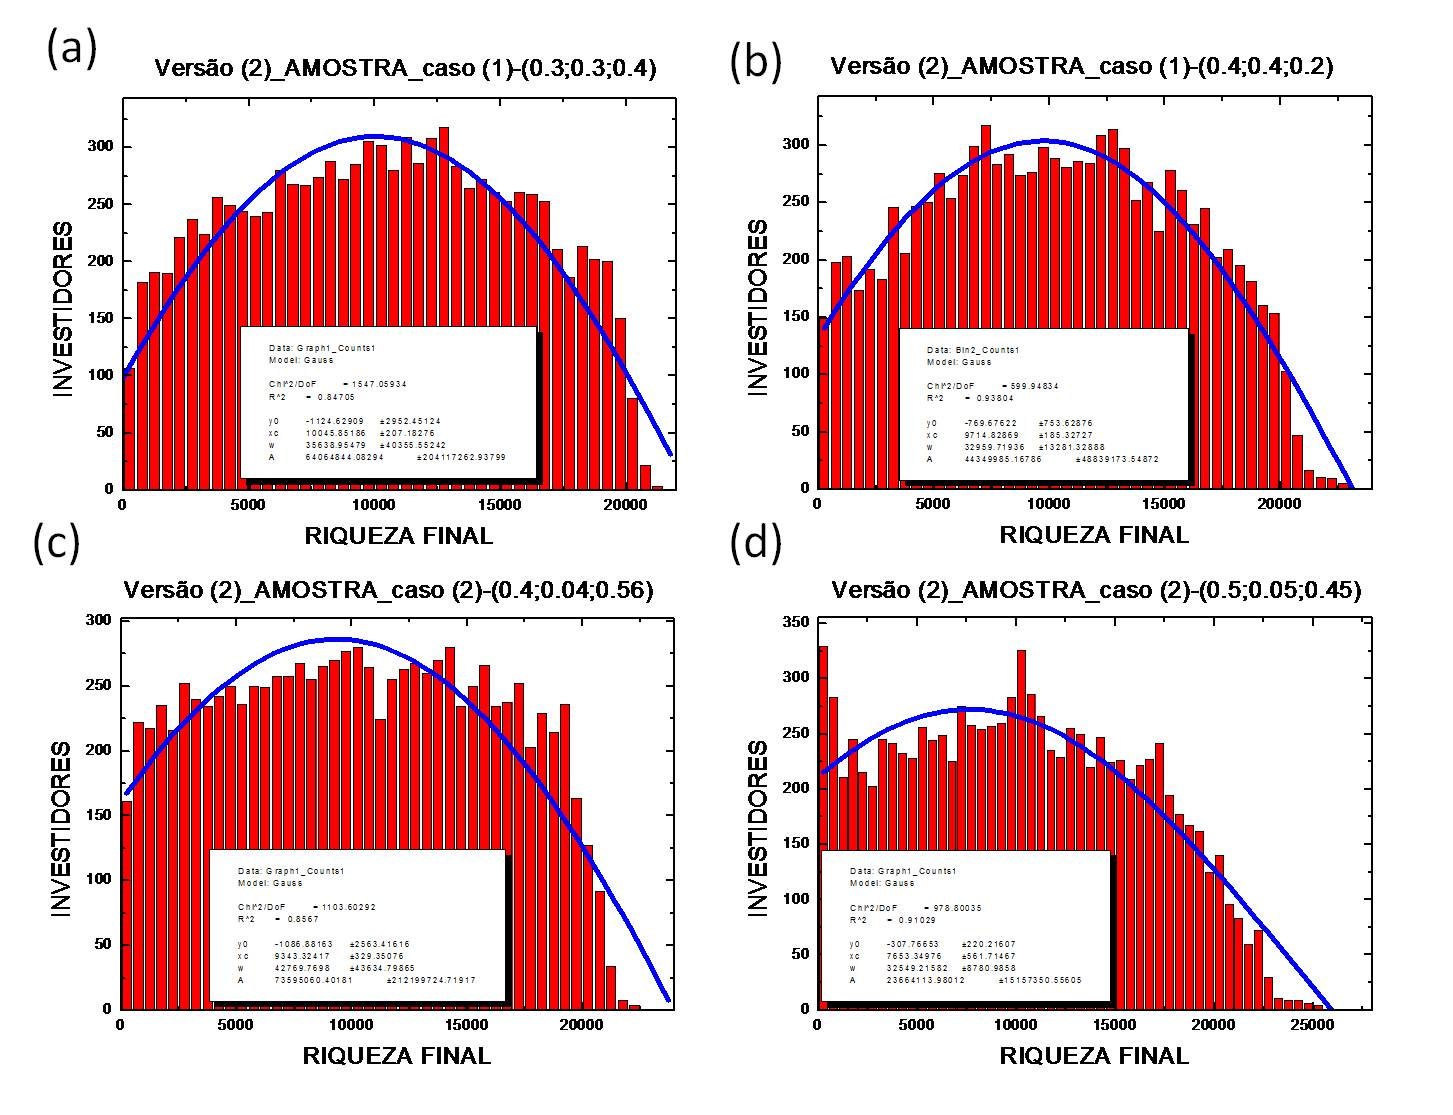
\includegraphics[width=0.8\linewidth]{Figuras/16.jpg}
\caption [Histograma da distribuição final do dinheiro dos investidores em
RLT]{Histograma da distribuição final do dinheiro dos investidores em RLT.
(Cálculo feito pela
quantidade final de ações vezes o índice atual, somado a quantidade final de
dinheiro). As figuras (a) e (b) representam o caso (1), (c) e (d) o caso (2).}
\label{fig:histograma}
\end{figure}

Em RLT.3, mesmo limitando a quantidade de dinheiro e o número de ações o
índice do mercado não varia muito (não tem grandes flutuações), mantendo-se bem
parecido com o RIT.3. Por causa dessa semelhança não iremos expor seus gráficos.


Ao analisar o histograma da distribuição final do dinheiro dos investidores em
RLT, representado na figura \ref{fig:histograma},
observamos à medida que $P_1$ e $P_2$ aumentam o número de falidos também
aumenta. Comparando RLT.2 com RLT.1 pelas figuras \ref{fig:histograma}(b) e
\ref{fig:histograma}(c), verificamos que o aumento de falidos em RLT.2 é maior,
assim, concluímos que $P_1$ é que mais influência nesse aumento. Pois em RLT.2 
o número de imitadores é 10 vezes maior do que em RLT.1 . Em todos os casos as
distribuições aproximaram-se levemente de uma gaussiana.  


\begin{figure}[!h]
\centering
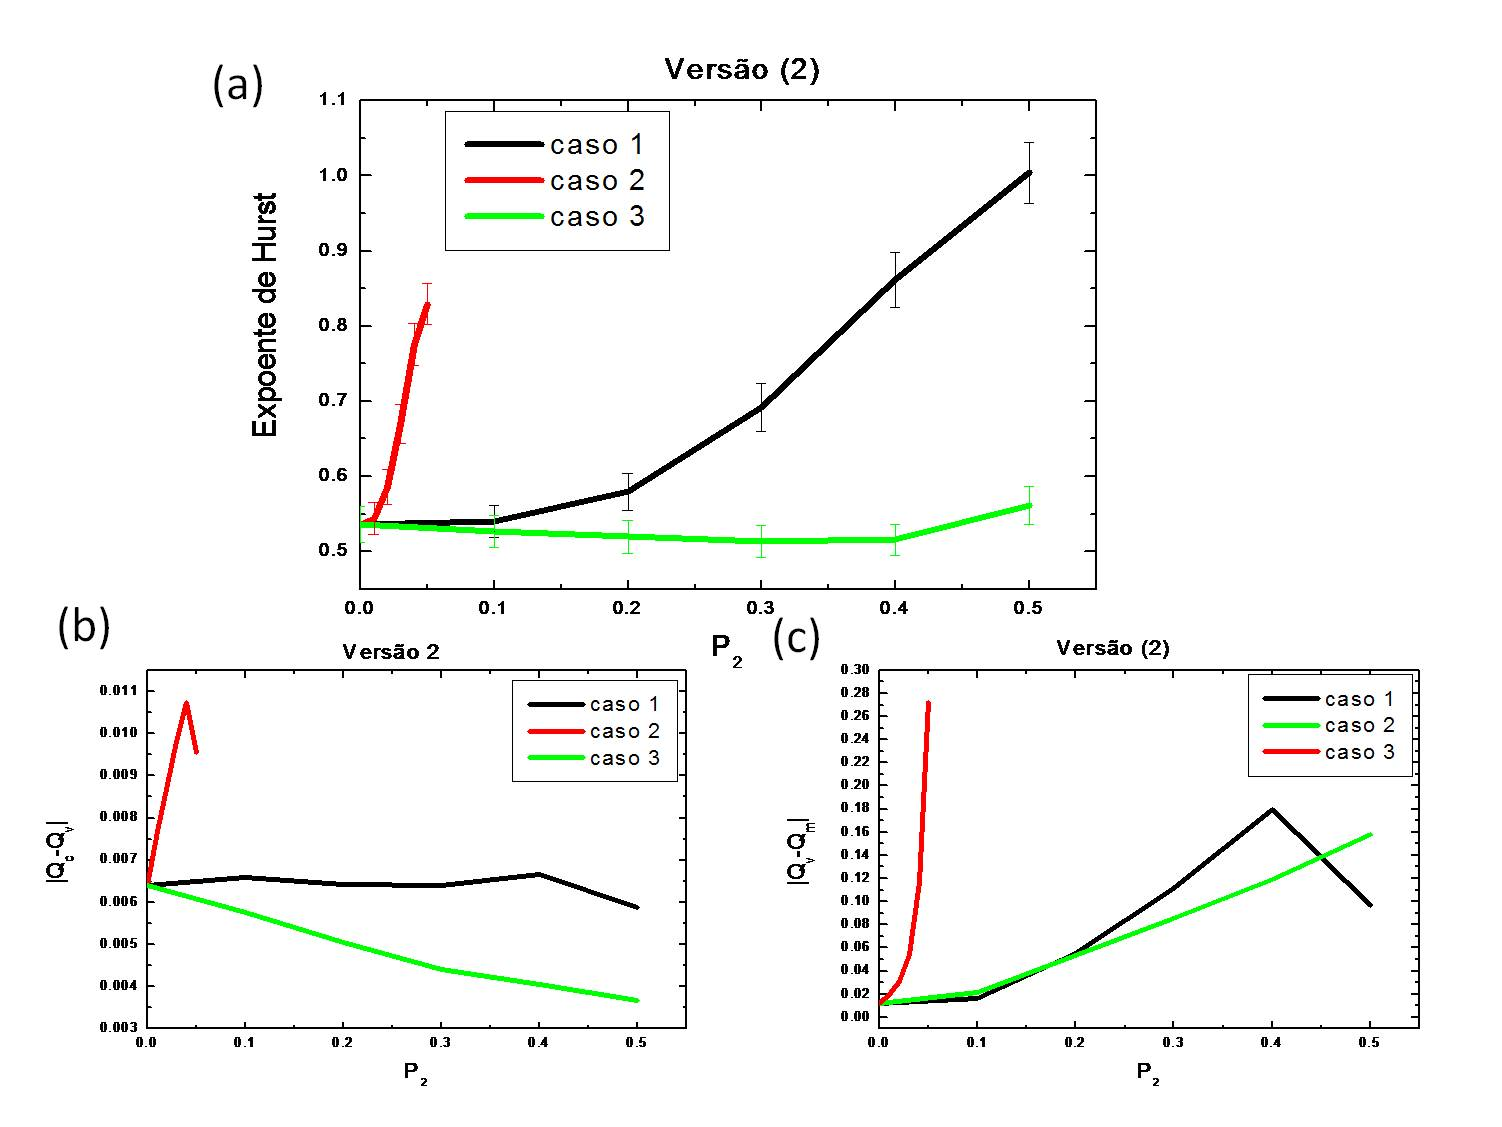
\includegraphics[width=0.8\linewidth]{Figuras/17.jpg}
\caption[Análise do expoente de Hurst em RLT]{Na figura 5.11.a é representado no
gráfico o valor médio das 1000 amostras do expoente de Hurst em RLT para cada
caso em função de $P_2$.
Na figura \ref{fig:valor-medio}(b) é representada a porcentagem da diferença
entre o número de pessoas que estão comprando ($Q_b$) e as que estão vendendo
($Q_s$) (cálculo do efeito médio de manada para os estados comprar ou vender)
em função de $P_2$. Na figura \ref{fig:valor-medio}(c) é representada da
diferença entre o número de pessoas que estão no estado comprar ($Q_b$) e as que
estão estado vender ($Q_h$) (que é igual à diferença entre o número pessoas que
estão vendendo e as que estão mantendo) em função de $P_2$, ou seja, é calculada
a porcentagem da diminuição da escolha ``manter''.}
\label{fig:grafico2}
\end{figure}

Observamos, na figura \ref{fig:grafico2}, que as porcentagens médias do
efeito de manada, geralmente, são menores do que em RI. Como conseqüência disso,
o valor do expoente de Hurst, em RLT.1 e RLT.2 são menores do que em RIT.1 e
RIT.2, respectivamente.  Já em RLT.3  o valor médio é semelhante a RIT.3 .   A
limitação do dinheiro e das ações faz a diferença entre as pessoas que estão
comprando e vendendo tendem para escolha manter, quando ficam sem dinheiro ou
ações, como observado em \ref{fig:grafico2}. Em todos os casos em RLT o
efeito de “manada” representado em \ref{fig:grafico2} é menor em todos os casos
representados em RIT, relação que também é consequência da limitação do
dinheiro. Aparentemente, o efeito
que mais influencia no expoente de Hurst é o efeito manda, como observado em
\ref{fig:grafico2}(b).

Em RLT.1, o aumento de $P_1$ (investidores imitadores) também aumenta a
tendência para $H>(1/2)$, sendo que na maioria das situações esse aumento é
menor
do que em RIT.1. A única situação em que o expoente de Hurst em RLT.1 é maior do
que em RIT.1 é o T.1-(0.5;0.5;0), na qual o percentual de indiferentes é zero. 

Em RLT.2, em que a porcentagem de investidores imitadores é 10 vezes maior que a
de investidores anti-imitadores, o efeito manada aumenta à medida que P1
aumenta, mais rapidamente que nos outros casos em RLT, relação que já foi
observada no RIT.2. Já o valor do expoente de Hurst é menor em todos as
situações comparado a RIC.2. 


Em RLT.3, observamos a mesma tendência do RIT.3. O valor $H\sim (1/2)$, o que é
esperado para um mercado eficiente. Mesmo com o aumento de $P_2$ e com a
diminuição do número de investidores que estão no estado manter, o expoente
Hurst varia pouco.


Assim, concluímos que os valores do expoente de Hurst estão mais próximos do
mercado real em RLT.1, RLT.2 e RLT.3.

\begin{figure}[!h]
\centering
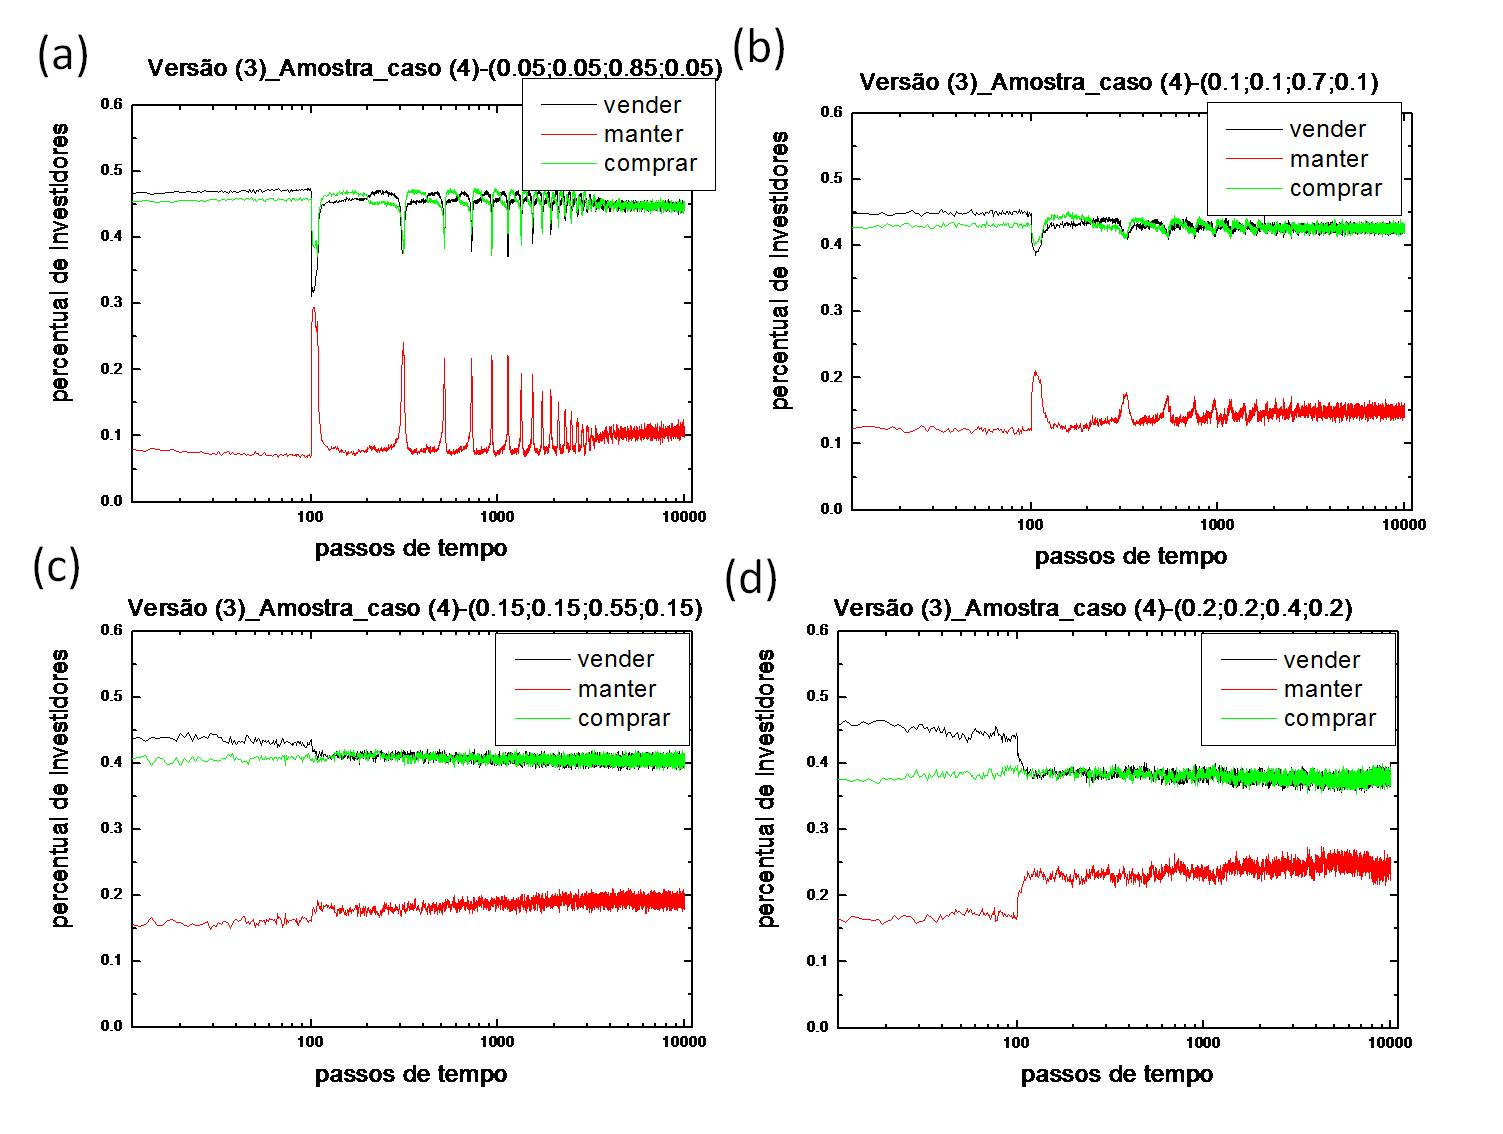
\includegraphics[width=0.8\linewidth]{Figuras/18.jpg}
\caption[Evolução do comportamento dos investidores em RLQ.1]{Evolução do
comportamento dos investidores durante o tempo em RLQ.1 de uma amostra.
Definimos a mesma escala da representação da variação do percentual, em 0 a 0.6.
}
\label{fig:evolucao-comp-investidores3}
\end{figure}

\section{RLQ}

Na simulação da versão (3), RLQ, semelhante à RLT, a quantidade
de dinheiro e ações é finita, sendo seus valores iniciais, 10000 e 100,
respectivamente. Além dos três tipos de investidores, consideramos um quarto
tipo denominado “imitador do mais rico”.  Como temos quatro tipos de
investidores, os casos simulados são os Q.1, Q.2 e Q.3.

\begin{figure}[!h]
\centering
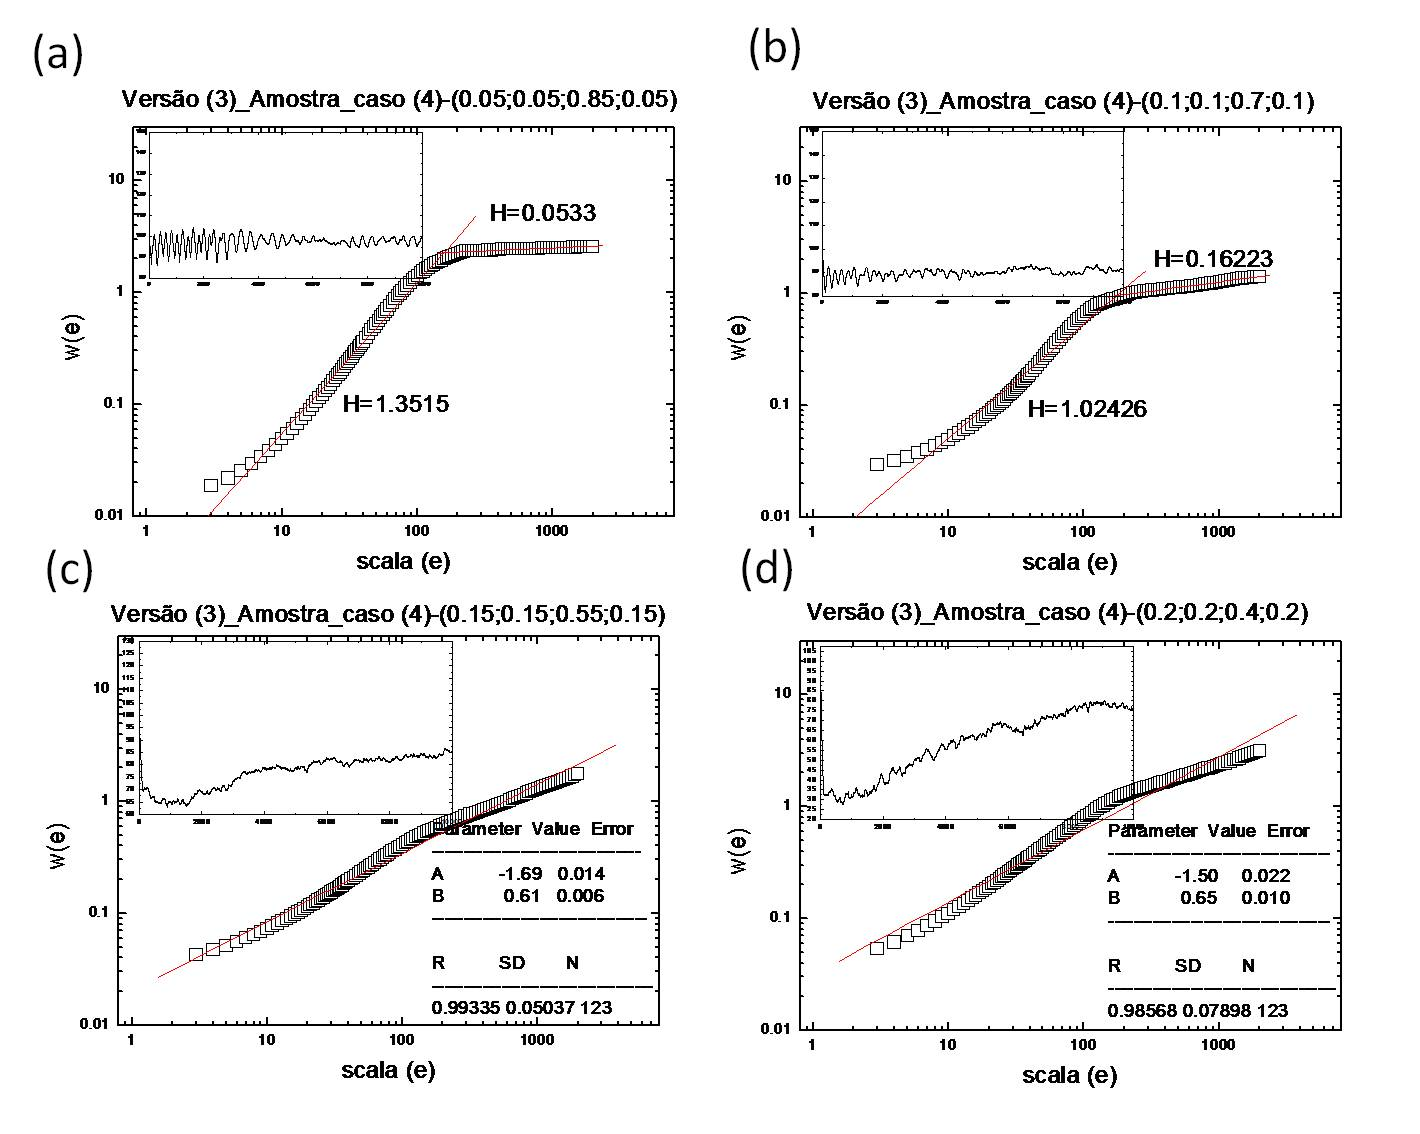
\includegraphics[width=0.8\linewidth]{Figuras/19.jpg}
\caption [Cálculo do expoente de Hurst para os índices em RLQ 1]{Cálculo do
expoente de Hurst para os índices das ações de uma amostra produzidas em RLQ 1.
O parâmetro B representa o valor de H.
Nos detalhes em cada painel são mostrados os gráficos do índice das ações. Em
(a) e (b) representamos os índices variando de 80 a 150, já em (c) variando de
60 a 130 e em (d) de 20 a 105. }
\label{fig:calculo-expoente-hurst7}
\end{figure}

Em RLQ.1, em todas as situações, nos primeiros passos de tempo, observamos um
efeito de manada para a escolha vender, exemplificado na figura
\ref{fig:evolucao-comp-investidores3}. Em
\ref{fig:evolucao-comp-investidores3}(a) e
\ref{fig:evolucao-comp-investidores3}(b) , é observado um efeito interessante,
principalmente em \ref{fig:evolucao-comp-investidores3}(a) os
investidores rapidamente se recuperam de suas perdas, ou seja, os investidores
que ficam sem dinheiro ou ações, em pouco tempo, voltam a participar do mercado,
comprando e vendendo ações normalmente. Quem ficou sem dinheiro (ou sem ações) e
tem ações (ou dinheiro) começa a vendê-las (ou a comprá-las); normalizando sua
situação; fica claro esse efeito em \ref{fig:calculo-expoente-hurst7}(a),
índice referente a essa situação, que sobe e rapidamente desce.  Já em
\ref{fig:evolucao-comp-investidores3}(c) e (d), depois de certo número passos de
tempo, à medida que $P_1$ e $P_4$ aumentam, o número de investidores falidos
aumenta também, principalmente em \ref{fig:evolucao-comp-investidores3}(d),
fato que também influencia no aumento das flutuações do mercado, como em
\ref{fig:calculo-expoente-hurst7}(c) e (d). No cálculo do expoente de
Hurst, em \ref{fig:calculo-expoente-hurst7} (a) e (b), a reta apresenta
duas inclinações, indicando dois comportamentos diferentes do índice do mercado,
relação comutada acima.

\begin{figure}[!h]
\centering
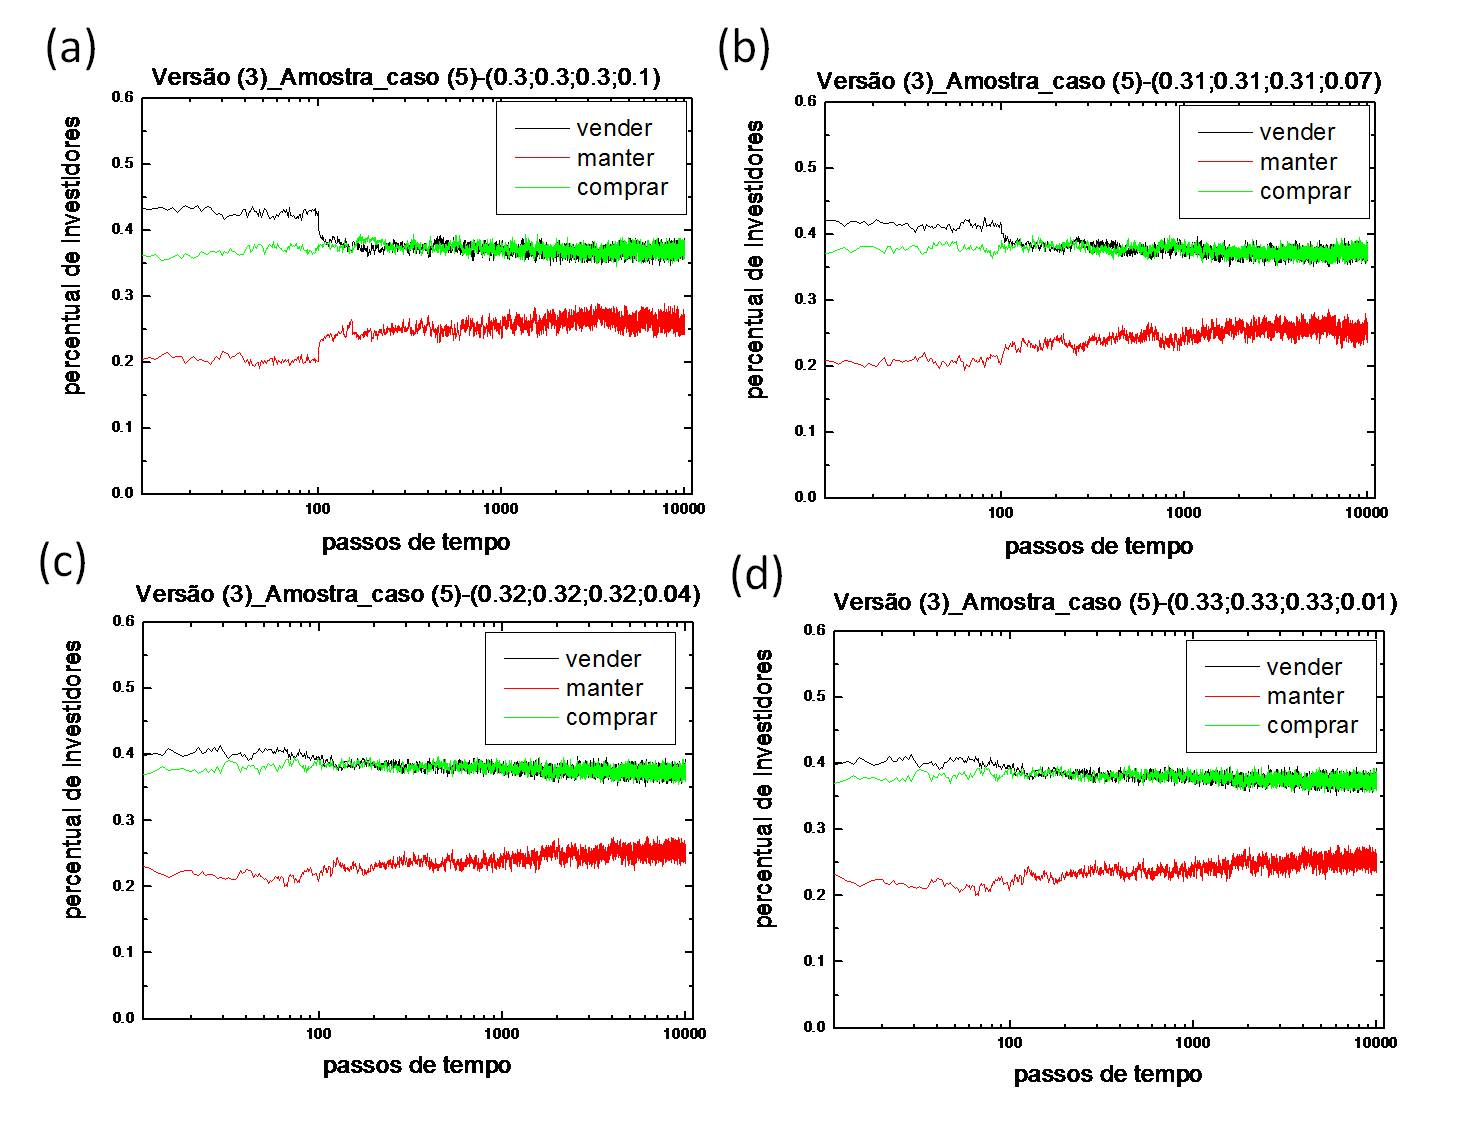
\includegraphics[width=0.8\linewidth]{Figuras/20.jpg}
\caption [Evolução do comportamento dos investidores em RLQ.2]{Evolução do
comportamento dos investidores durante o tempo em RLQ.2 de uma amostra.
Definimos a mesma escala da representação da variação do percentual, em 0 a
0.6. }
\label{fig:evolucao-comp-investidores4}
\end{figure}

\begin{figure}[!h]
\centering
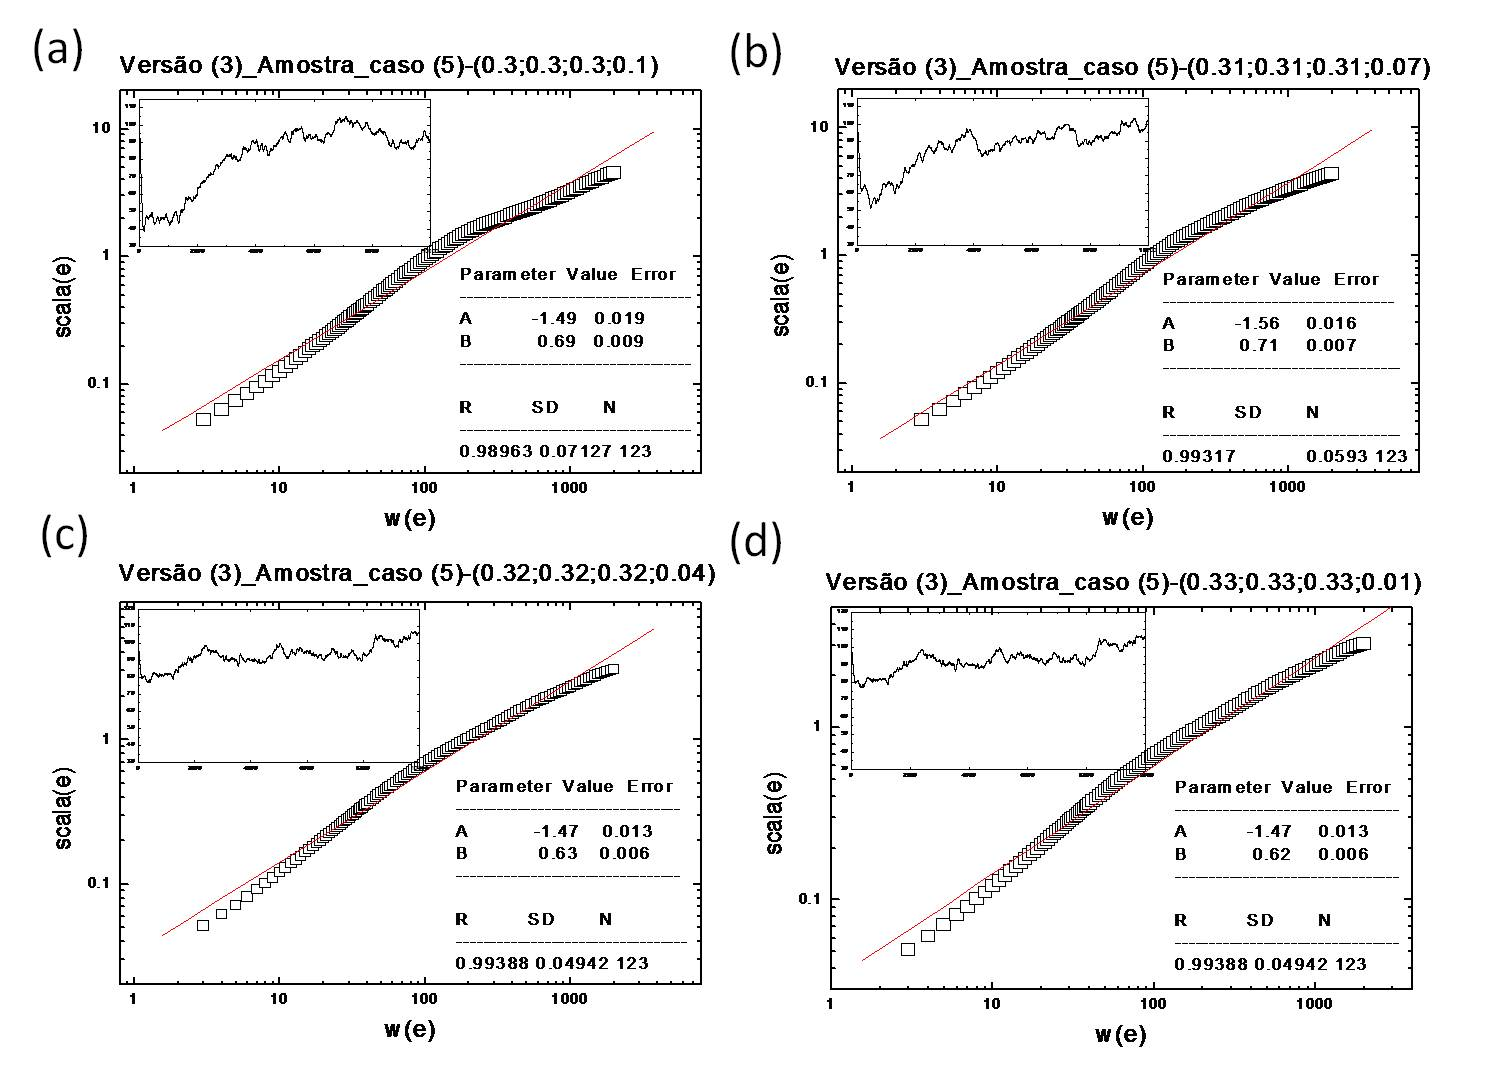
\includegraphics[width=0.8\linewidth]{Figuras/21.jpg}
\caption[Cálculo do expoente de Hurst para os índices em RLQ.2]{Cálculo do
expoente de Hurst para os índices das ações de uma amostra
produzidas em RLQ.2.  O parâmetro B representa o valor de H.
Nos detalhes em cada painel são mostrados os gráficos do índice das ações. Em
todas as situações representamos os índices variando de 30 a 120. }
\label{fig:calculo-exp-hurst8}
\end{figure}

Em RLQ.2, em todas as situações, nos primeiros passos de tempo, observamos
também um efeito de manada para a escolha vender, exemplificado na figura
\ref{fig:evolucao-comp-investidores4} principalmente, para as situações em que
$P_1 + P_4$ possuem os maiores valores. Verificamos também que esse aumento de
P1 + P4 influencia no aumento de pessoas que escolhem manter, depois de certo
número de passos de tempo, como exemplificado em
\ref{fig:evolucao-comp-investidores4} (a) e (b). Assim,  algumas
delas ficam sem dinheiro ou ações em determinado tempo ou até o final da
simulação. Esse efeito de manada aumenta também as flutuações do mercado,
principalmente em \ref{fig:calculo-exp-hurst8} (a) e (b).



\begin{figure}[!h]
\centering
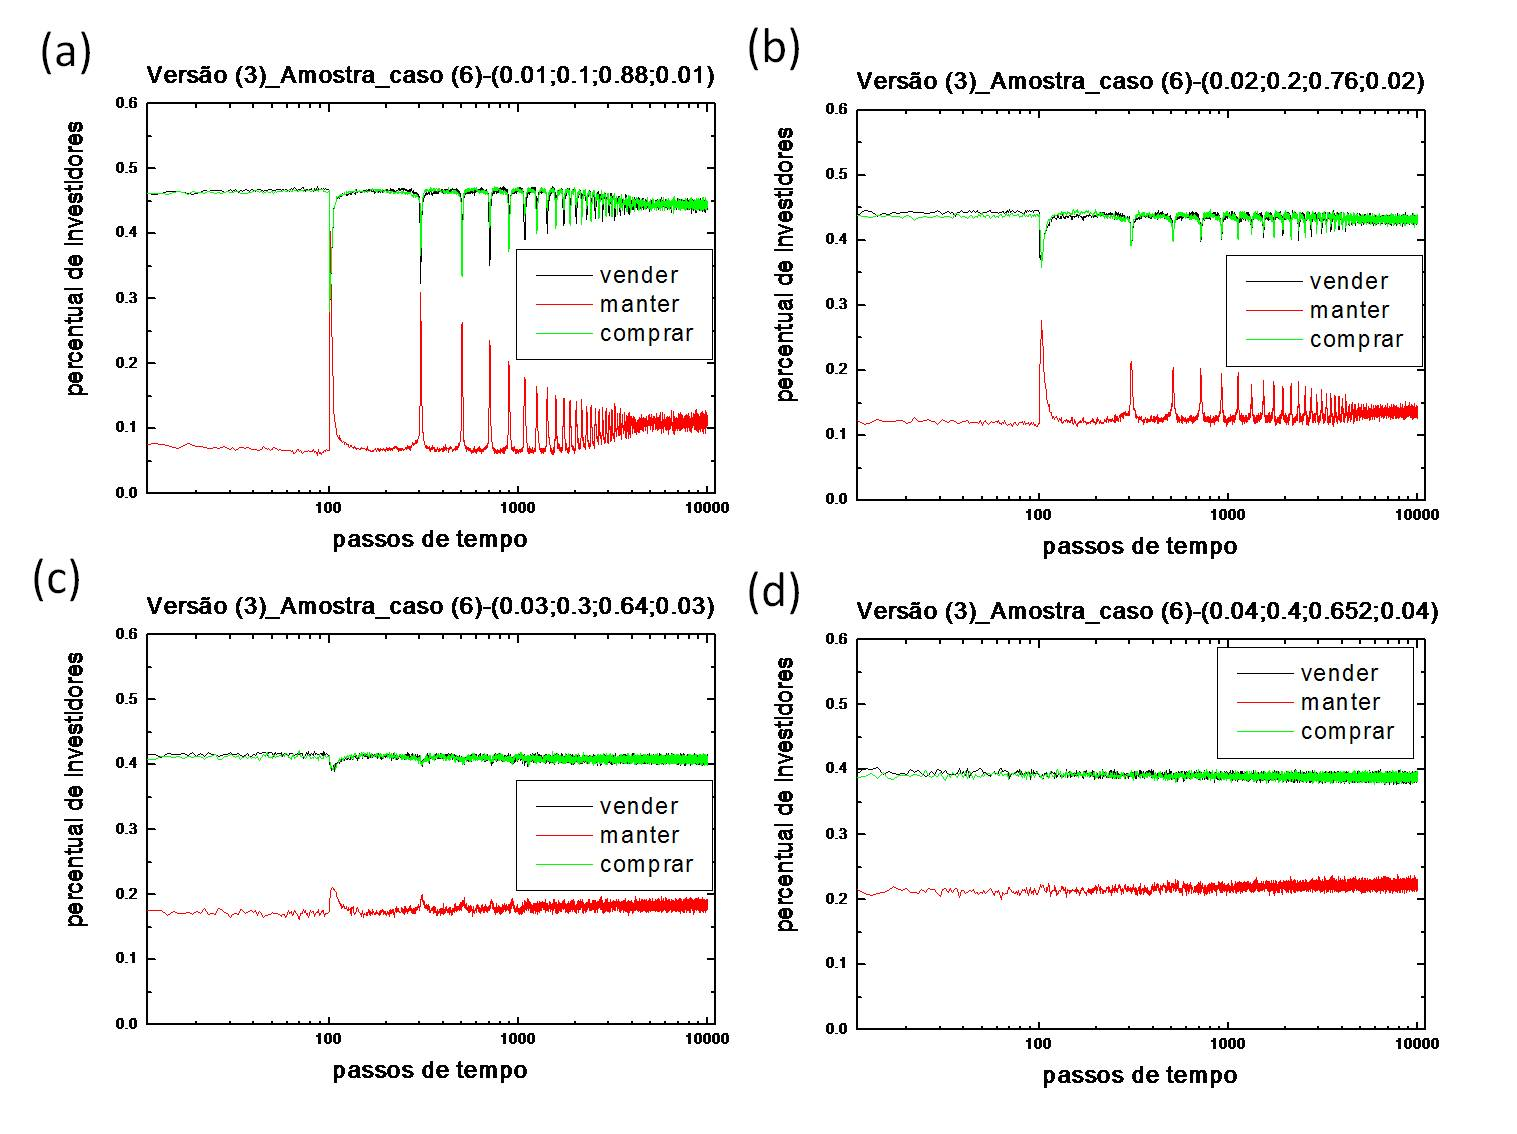
\includegraphics[width=0.8\linewidth]{Figuras/22.jpg}
\caption [Evolução do comportamento dos investidores em RLQ.3]{Evolução do
comportamento dos investidores durante o tempo em RLQ.3 de uma amostra.
Definimos a mesma escala da representação da
variação do percentual, em 0 a 0.6.  }
\label{fig:evolucao-comp-investidores5}
\end{figure}

\begin{figure}[!h]
\centering
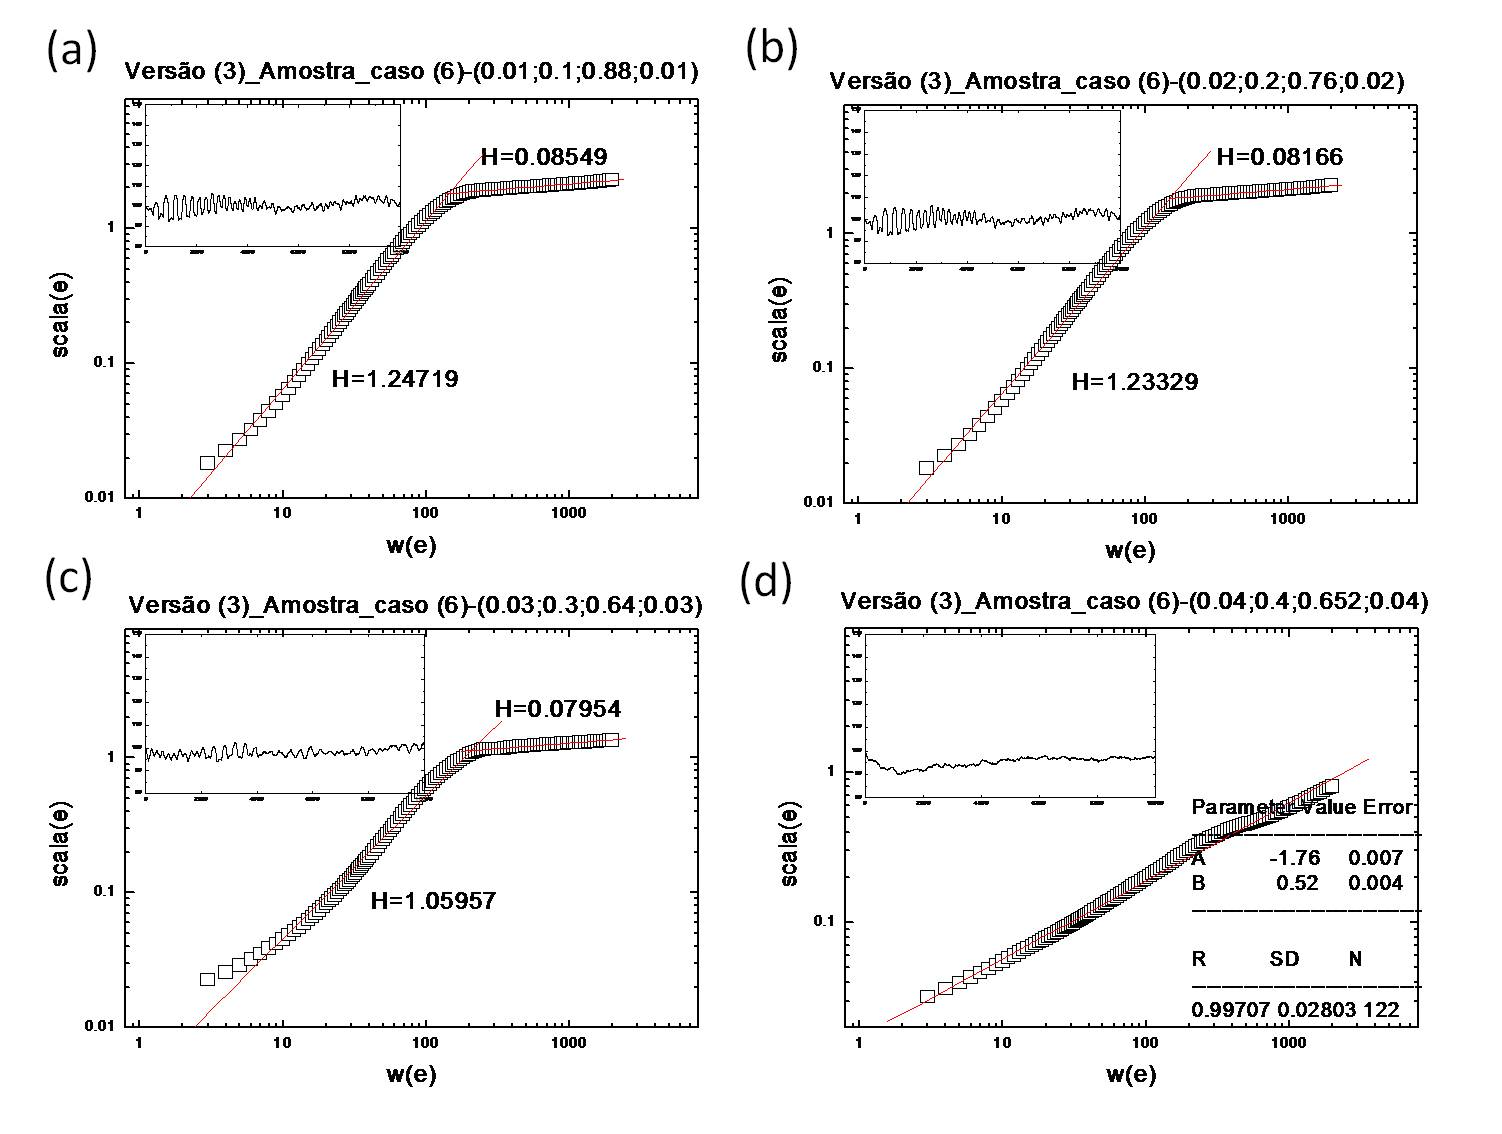
\includegraphics[width=0.8\linewidth]{Figuras/23.jpg}
\caption[Cálculo do expoente de Hurst para os índices em RLQ.3]{Cálculo do
expoente de Hurst para os índices das ações de uma amostra
produzidas em RLQ.3.  O parâmetro $B$ representa o valor de
$H$. Nos detalhes em cada painel são mostrados os gráficos do índice das ações.
Em todas as situações representamos os índices variando de 80 a 150.}
\label{fig:calculo-exp-hurst9}
\end{figure}

Em RLQ.3, os valores de $P_1$ e $P_4$ são pequenos, assim não há efeito de
manada entre as escolhas comprar ou vender, mas à medida que $P_1$ e $P_4$
aumentam, alguns investidores  começam a optar pela escolha manter,
principalmente em \ref{fig:evolucao-comp-investidores5}(c) e (d), indicando que
ficaram sem dinheiro ou ações. Semelhante ao RLQ.1, principalmente, em
\ref{fig:evolucao-comp-investidores5}(a) e (b), é observado o mesmo efeito
 quando P4 é pequeno, influenciando também os índices referentes a
essas situações, principalmente em \ref{fig:calculo-exp-hurst9} (a) e (b), em
que há vários movimentos de sobe e desce, mas em pequenas flutuações, em curtos
intervalos de tempo. Em \ref{fig:calculo-exp-hurst9}(d), temos o mercado mais
estável de RLQ.1, onde temos o maior valor de P2+P3 entre todas as situações.
No cálculo do expoente de Hurst, em \ref{fig:calculo-exp-hurst9}(a), (b) e (c),
a reta também apresenta duas inclinações, indicando dois comportamentos
diferentes do índice do mercado, ou seja, em escalas curtas de tempo o índice
apresentava grandes flutuações, mas que começam a diminuir, oscilando
muito menos, quando observado em grandes escalas de tempo.

Observamos, no geral, que a influência de $P_4$ é grande comparada às versões
RI e RL (em que $P_4$ não existe). Quando seu valor é pequeno, causa efeitos
interessantes que não acontecem na versão (2). E ,quando é grande, seu valor
influencia mais no efeito manada que  $P_1$.


\begin{figure}[!h]
\centering
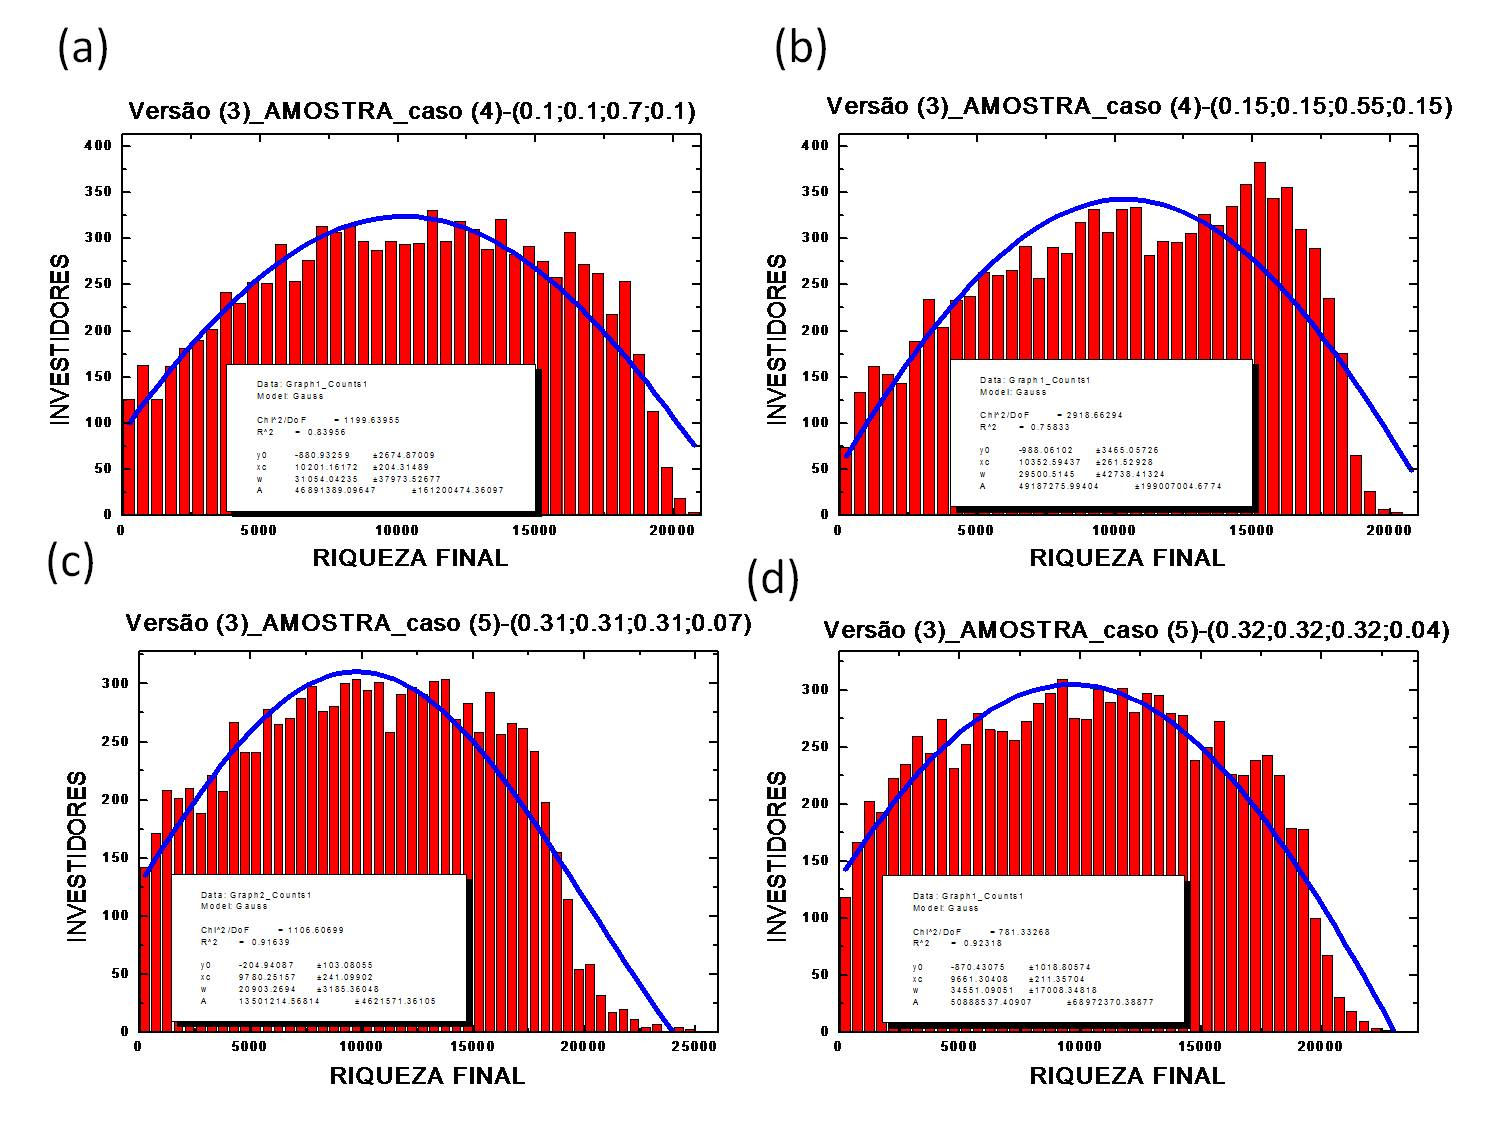
\includegraphics[width=0.8\linewidth]{Figuras/24.jpg}
\caption[Histograma da distribuição final do dinheiro dos investidores em
RLQ]{Histograma da distribuição final do dinheiro dos investidores em RLQ.
(Cálculo feito pela
quantidade final de ações vezes o índice atual, somado a quantidade final de
dinheiro). As figuras (a) e (b) representam o caso (4), (c) e (d) o caso (5).}
\label{fig:histograma2}
\end{figure}

Ao analisar o histograma da distribuição final do dinheiro dos investidores em
RLQ, representado na figura \ref{fig:histograma2},
observamos também que em todos os casos as distribuições aproximaram-se
levemente  uma
gaussiana.  Verificamos que à medida que  $P_1 + P_4$ aumenta o número pessoas
que terminaram a simulação com menos de 10000 também aumenta. Assim, concluímos
que $P_1 + P_4$ possuem grande influência na distribuição do dinheiro final do
investidor.  


\begin{figure}[!h]
\centering
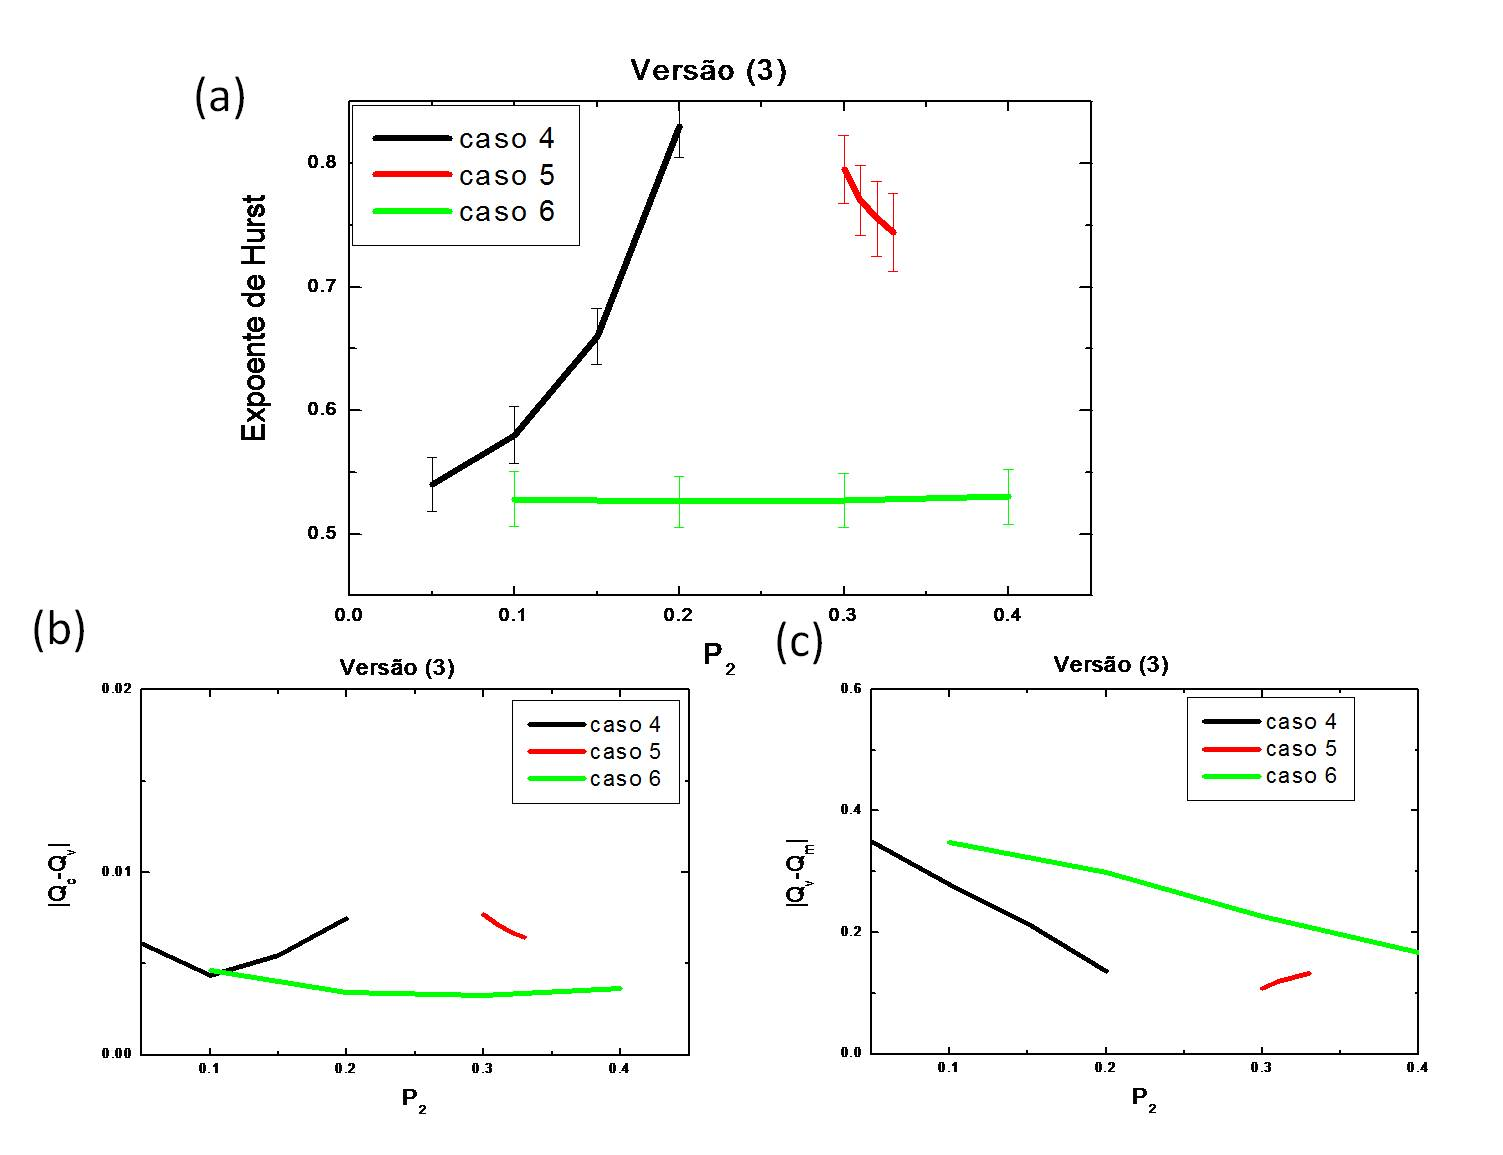
\includegraphics[width=0.8\linewidth]{Figuras/25.jpg}
\caption[Análise do expoente de Hurst em RLQ]{Na figura 5.11.a é representado
no
gráfico o valor médio das 1000 amostras do expoente de Hurst em RLQ para cada
caso em função de $P_2$.
Na figura \ref{fig:valor-medio}(b) é representada a porcentagem da diferença
entre o número de pessoas que estão comprando ($Q_b$) e as que estão vendendo
($Q_s$) (cálculo do efeito médio de manada para os estados comprar ou vender)
em função de $P_2$. Na figura \ref{fig:valor-medio}(c) é representada da
diferença entre o número de pessoas que estão no estado comprar ($Q_b$) e as que
estão estado vender ($Q_h$) (que é igual à diferença entre o número pessoas que
estão vendendo e as que estão mantendo) em função de $P_2$, ou seja, é calculada
a porcentagem da diminuição da escolha ``manter''.}
\label{fig:grafico3}
\end{figure}

Na figura 5.25, observamos que as porcentagens médias dos efeitos de
“manada”, geralmente, são maiores do que nas versões RIT e RLT. O valor máximo
do
expoente de Hurst é aproximadamente 0.83, observado em \ref{fig:grafico3}(a);
menor do que o máximo, na nas versões RI e RL. O efeito que mais correlaciona no
expoente de Hurst é o efeito de manada, como observado em \ref{fig:grafico3}. 


Em RLQ.1, o aumento de $P_1$ (investidores imitadores) juntamente com $P_4$
(imitador do mais rico) aumenta a tendência para $H>0,5$, que rapidamente fica
parecida com a dos mercados de países emergentes. 

Em RLQ.2,  a porcentagem de investidores imitadores somada à de 
imitadores do mais rico é maior que a de investidores anti-imitadores somada
aos indiferentes; o efeito manada aumenta à medida que $P_1+P_4$ aumenta, mais
rapidamente que nos outros casos, relação o que já foi observada e H converje
mais rápido para próximo de 0.8.  

Em RLQ.3, em que o número de anti-imitadores somado ao número de indiferentes
estão em maioria, observamos a tendência de $H\sim (1/2)$, o que é esperado para
um
mercado de países desenvolvidos. Mesmo com o aumento de $P_2$, e com a
diminuição do número de investidores que estão no estado manter, o expoente de
Hurst varia pouco.

Os valores do expoente de Hurst estão mais próximos do mercado real nessa
versão, comparada às duas primeiras versões. 

As versões (4) a (6) serão simuladas considerando-se redes aleatórias. Por
limitações computacionais, a extensão linear da rede é $L=90$, com $N=8100$ nós
(investidores). O número de vizinhos de cada investidor varia entre 5 e
30, como exemplificado no histograma do capitulo \ref{modelo}.

\begin{figure}[!h]
\centering
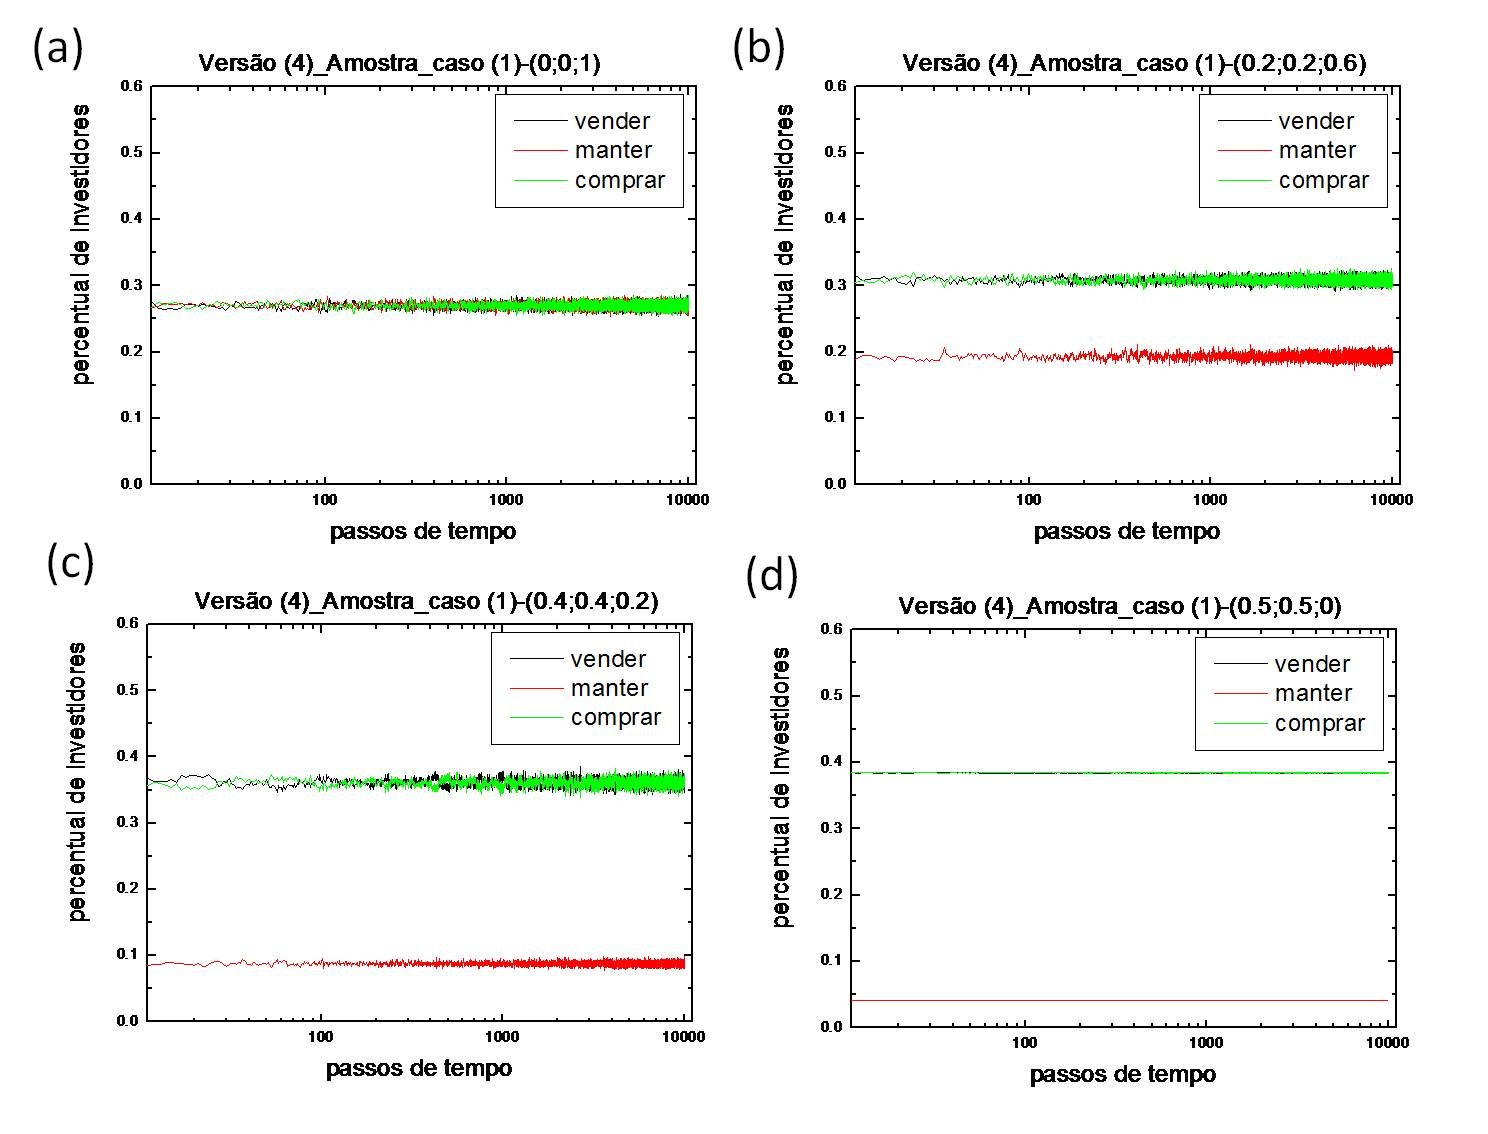
\includegraphics[width=.7\linewidth]{Figuras/26.jpg}
\caption[Evolução do comportamento dos investidores em AIT.1] {Evolução do
comportamento dos investidores durante o tempo em AIT.1 de uma amostra.
Definimos a mesma escala da representação da
variação do percentual, em 0 a 0,6. }
\label{fig:evolucao-comp-investidores6}
\end{figure}

\section{AIT}

Nessa quarta versão, a AIT, a rede é aleatória e a quantidade de dinheiro e
ações é ilimitada. Consideramos três tipos de comportamento para os
investidores.
O ''imitador'', o ''anti-imitador'' e o “indiferente”. Assim foram simulados os
casos  T.1, T.2 e T.3. 

\begin{figure}[!h]
\centering
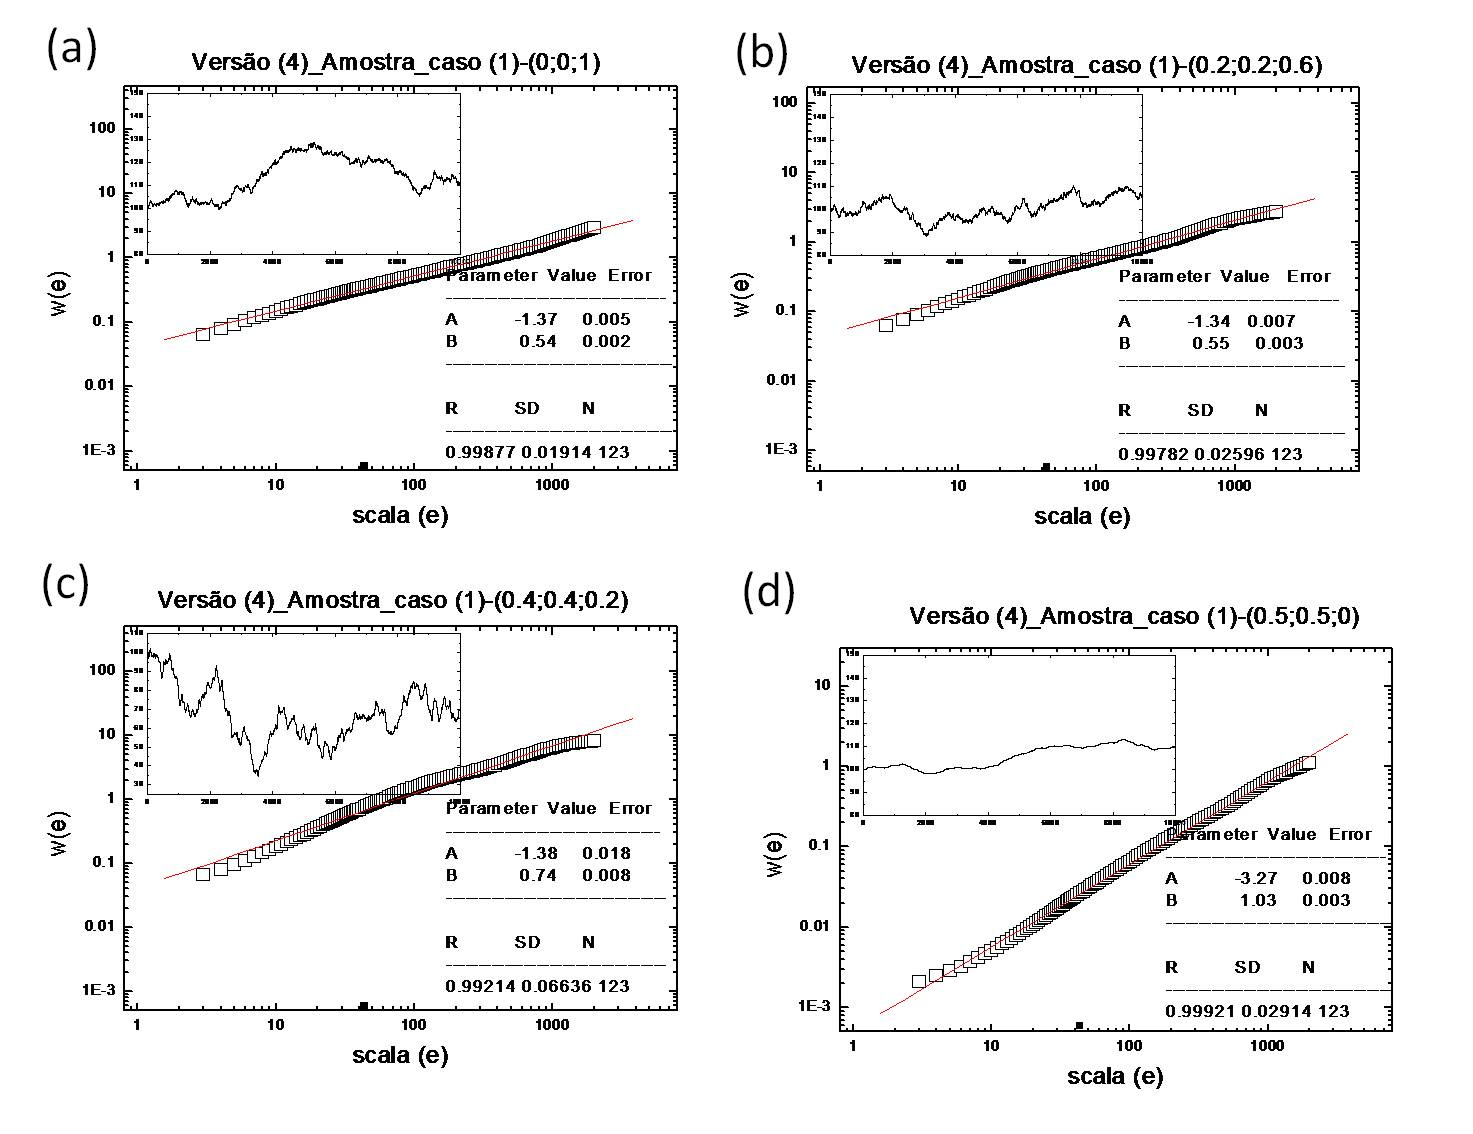
\includegraphics[width=.7\linewidth]{Figuras/27.jpg}
\caption [Cálculo do expoente de Hurst para os índices em AIT.1]{Cálculo do
expoente de Hurst para os índices das ações de uma amostra
produzidas em AIT.1.  O parâmetro $B$ representa o valor de
$H$. Nos detalhes em cada painel são mostrados os gráficos do índice das ações.
Em (a), (b) e (d)  a representação dos índices esta variando de 80 a 150 e em
(c) 30 a 110. }
\end{figure}

Em AIT.1, os resultados são semelhantes ao RIC.1; verifica-se que o número de
pessoas que estam vendendo e comprando
geralmente é proporcional, e que à medida que $P_2$ aumenta, o número de pessoas
que está mantendo diminui, como exemplificado na figura
\ref{fig:evolucao-comp-investidores6}. Observamos também grandes flutuações em
alguns índices,como em \ref{fig:evolucao-comp-investidores6} (c).

\begin{figure}[!h]
\centering
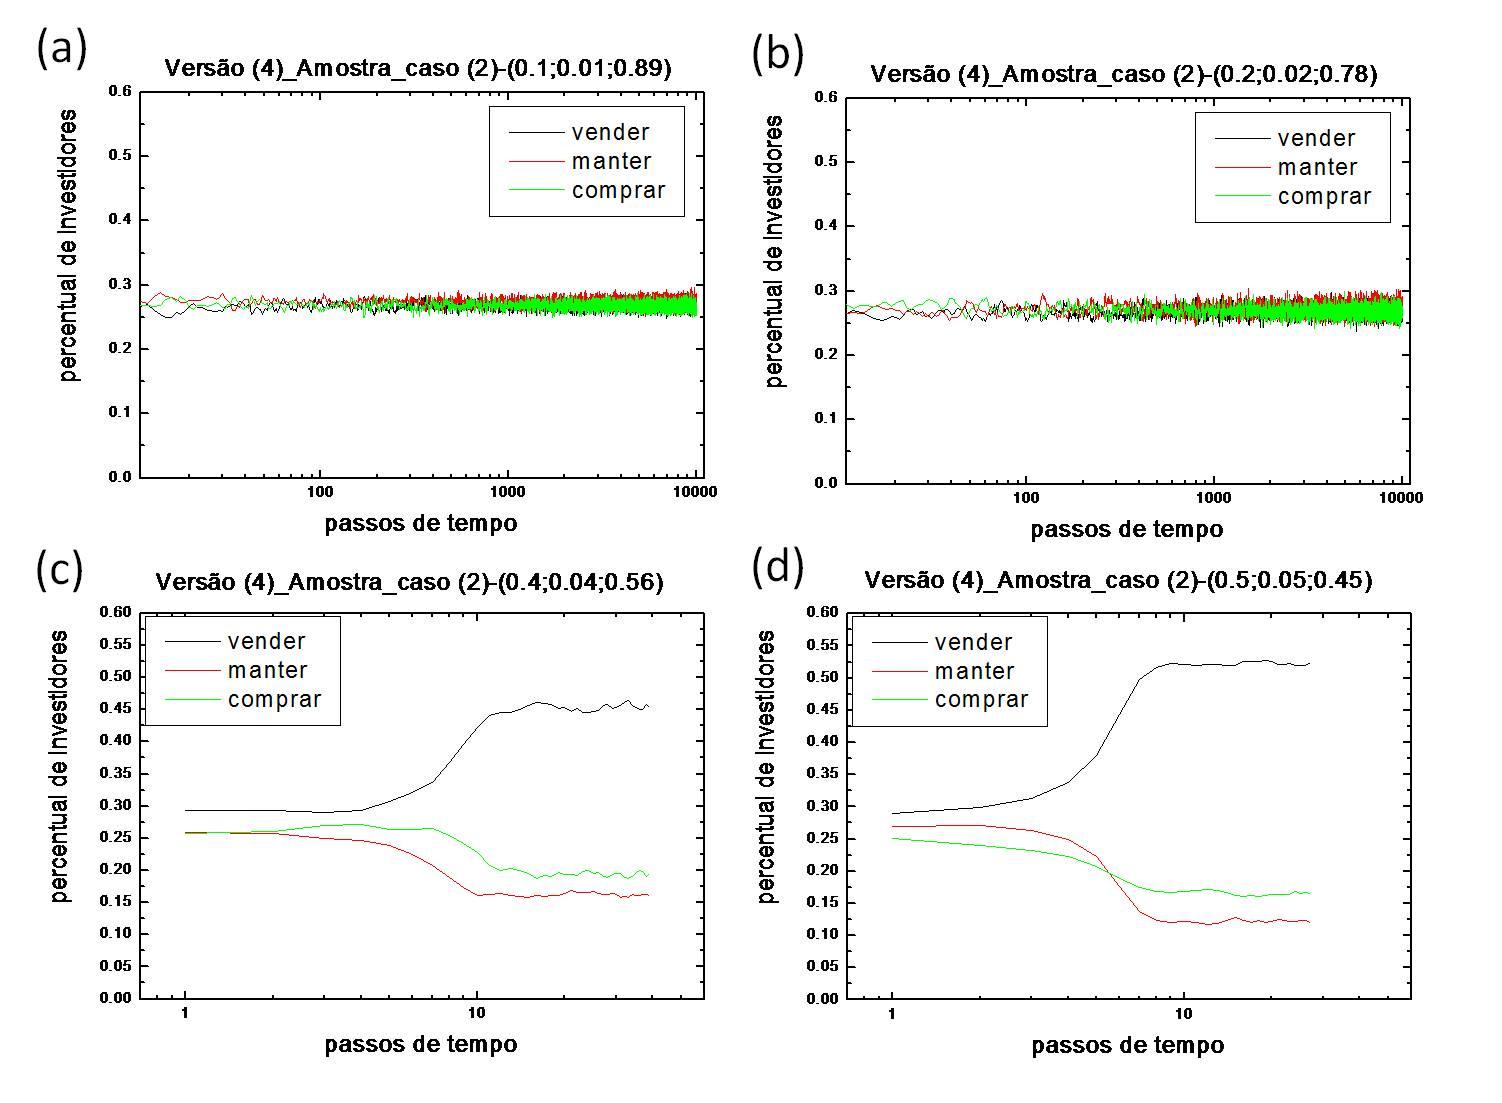
\includegraphics[width=.7\linewidth]{Figuras/28.jpg}
\caption{Evolução do comportamento dos investidores durante o tempo para caso
(2) na  versão (4) de uma amostra. Definimos a mesma escala da representação da
variação do percentual, em 0 a 0,6.  }
\label{fig:evolucao-comp-investidores7}
\end{figure}

\begin{figure}[!h]
\centering
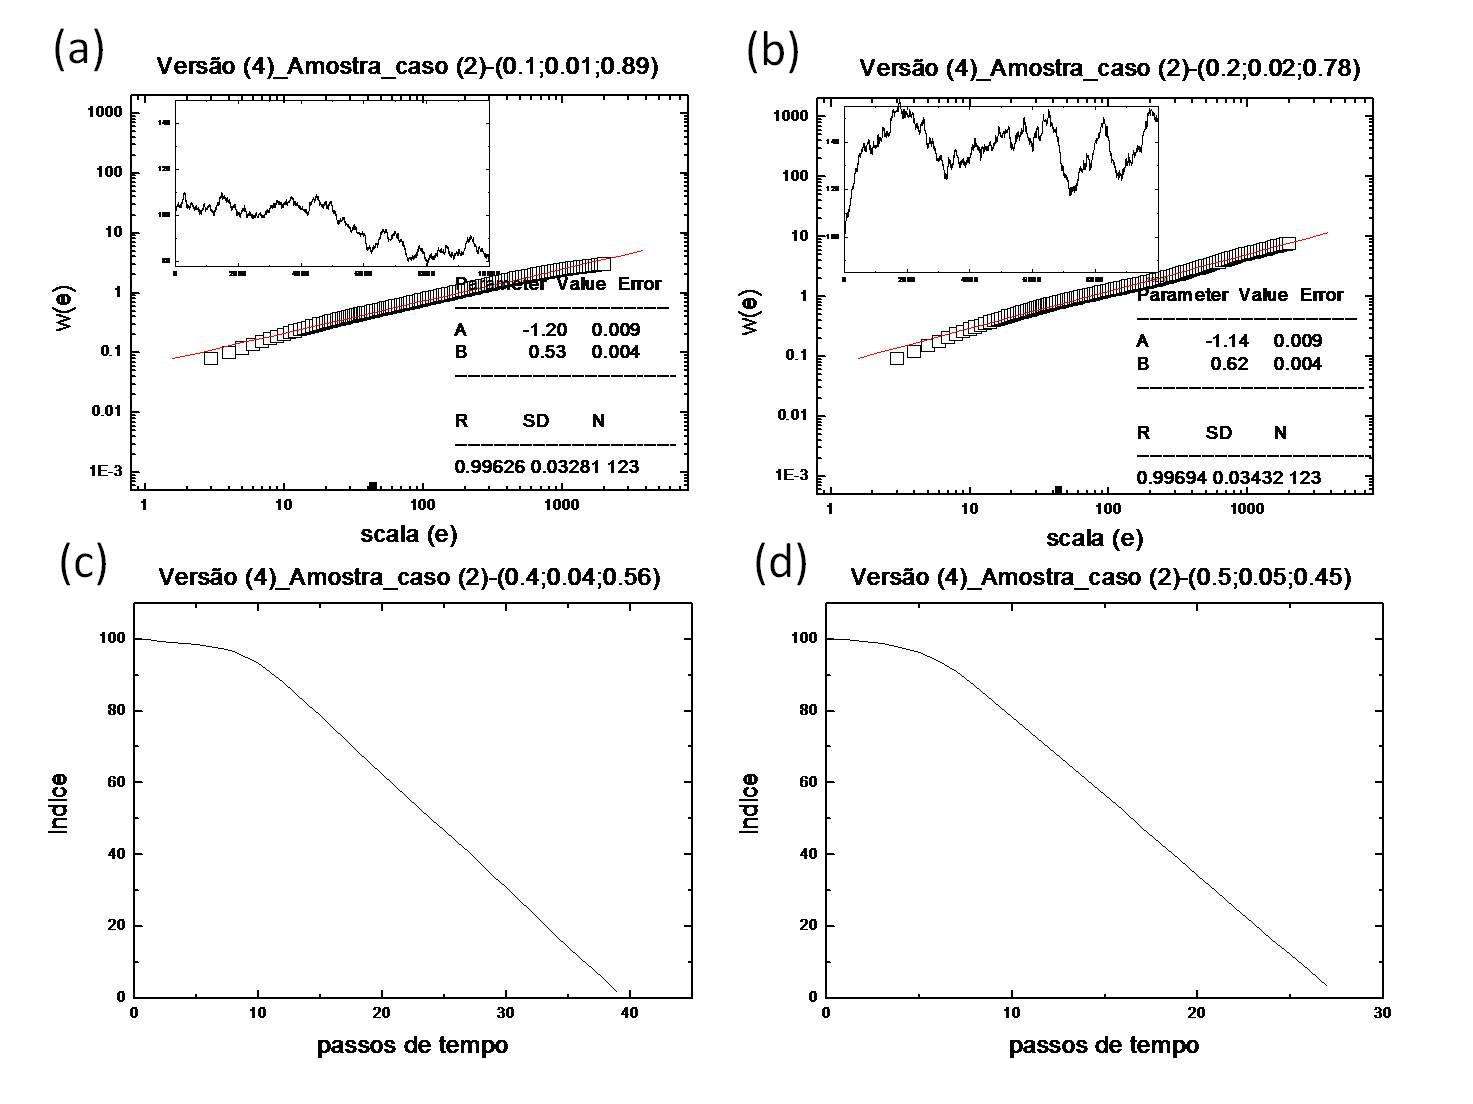
\includegraphics[width=.7\linewidth]{Figuras/29.jpg}
\caption{Em (a) e (b) Cálculo do expoente de Hurst para os índices das ações de
uma amostra produzidas no caso (2) na  versão (4).  O parâmetro $B$ representa o
valor de $H$. Nos detalhes em cada painel são mostrados os gráficos do índice
das ações. As representação dos índices esta variando de 80 a 150.  Em (c) e (d)
gráficos do índice das ações do caso (2) na versão (4). }
\label{fig:calculo-exp-hurst10}
\end{figure}

Em AIC.2, tem-se que, à medida que aumenta $P_1$, o efeito de
manada aumenta para as escolhas comprar ou vender; essa característica também
influencia no aumento das flutuações no mercado, como em
\ref{fig:evolucao-comp-investidores7} (c) e (d). O índice em
\ref{fig:calculo-exp-hurst10} (c) e (d), chega a quase zero em poucos passos de
tempo, ocorrendo assim a quebra do mercado. Sendo que em
\ref{fig:calculo-exp-hurst10} (d) esse efeito ocorre em menos tempo.
Como em AIC.1 não foi observado quebras, concluímos que o aumento de $P_1$
é o que mais afeta nesse acontecimento. Ressaltando que isso não ocorre RIC.2.

\begin{figure}[!h]
\centering
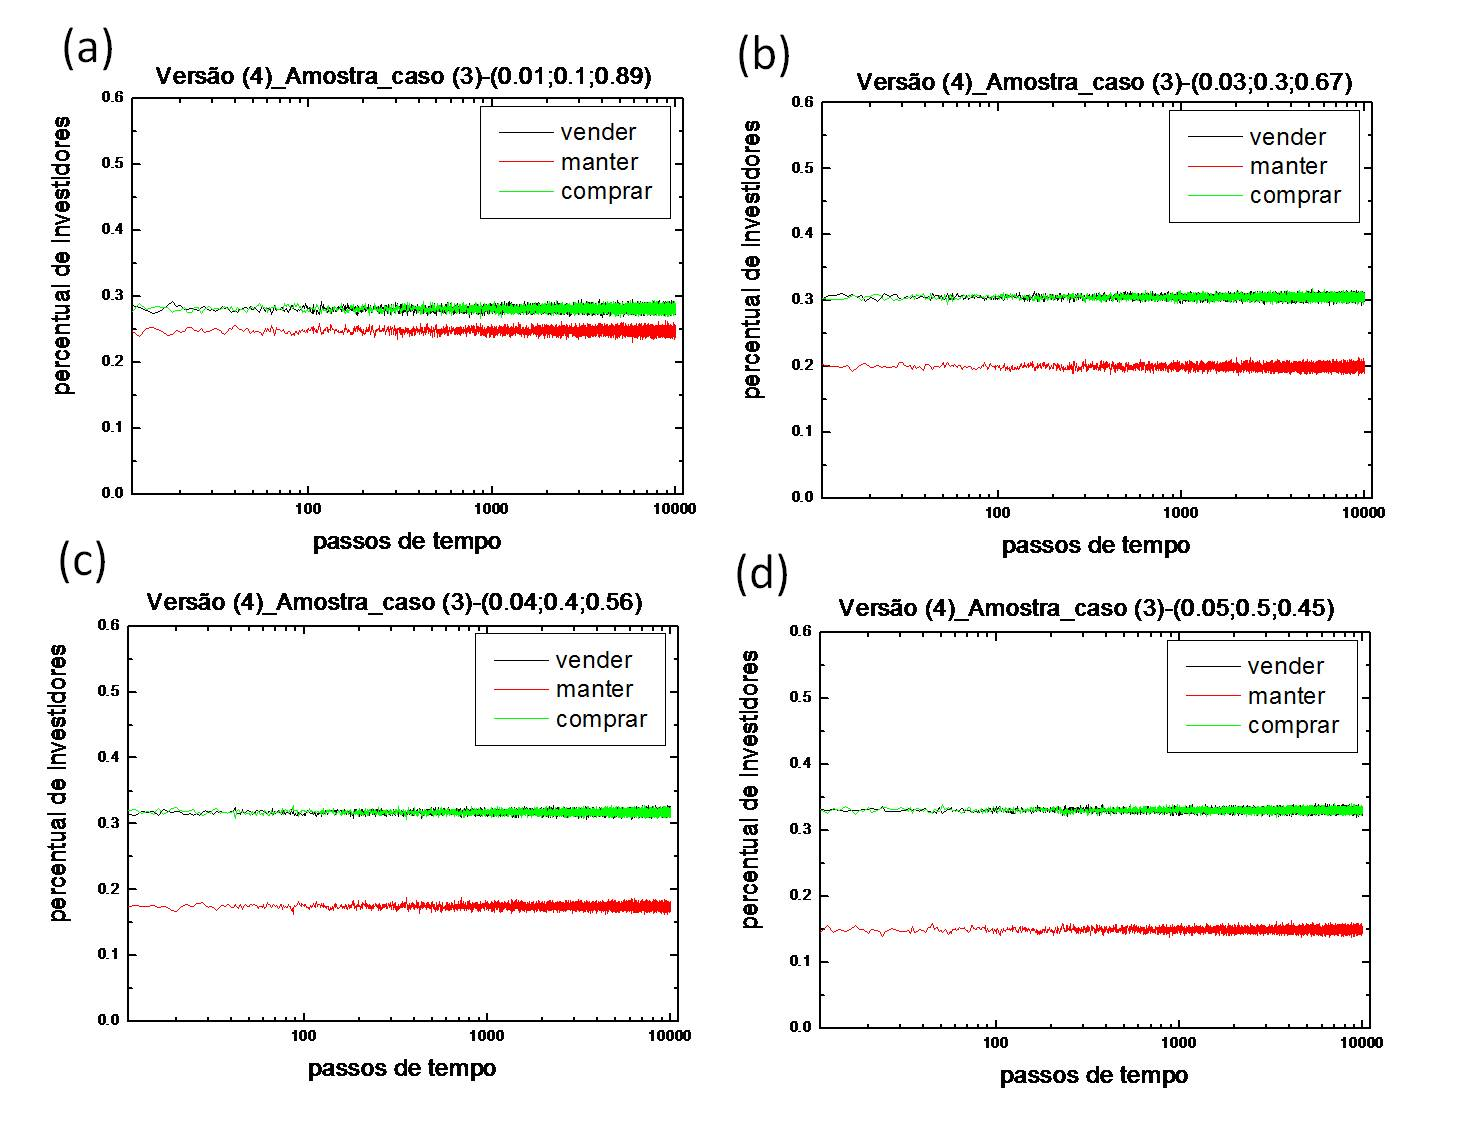
\includegraphics[width=.7\linewidth]{Figuras/30.jpg}
\caption{Evolução do comportamento dos investidores durante o tempo para caso
(3) na  versão (4) de uma amostra. Definimos a mesma escala da representação da
variação do percentual, em 0 a 0.6.  }
\label{fig:evolucao-comp-investidores8}
\end{figure}

\begin{figure}[!h]
\centering
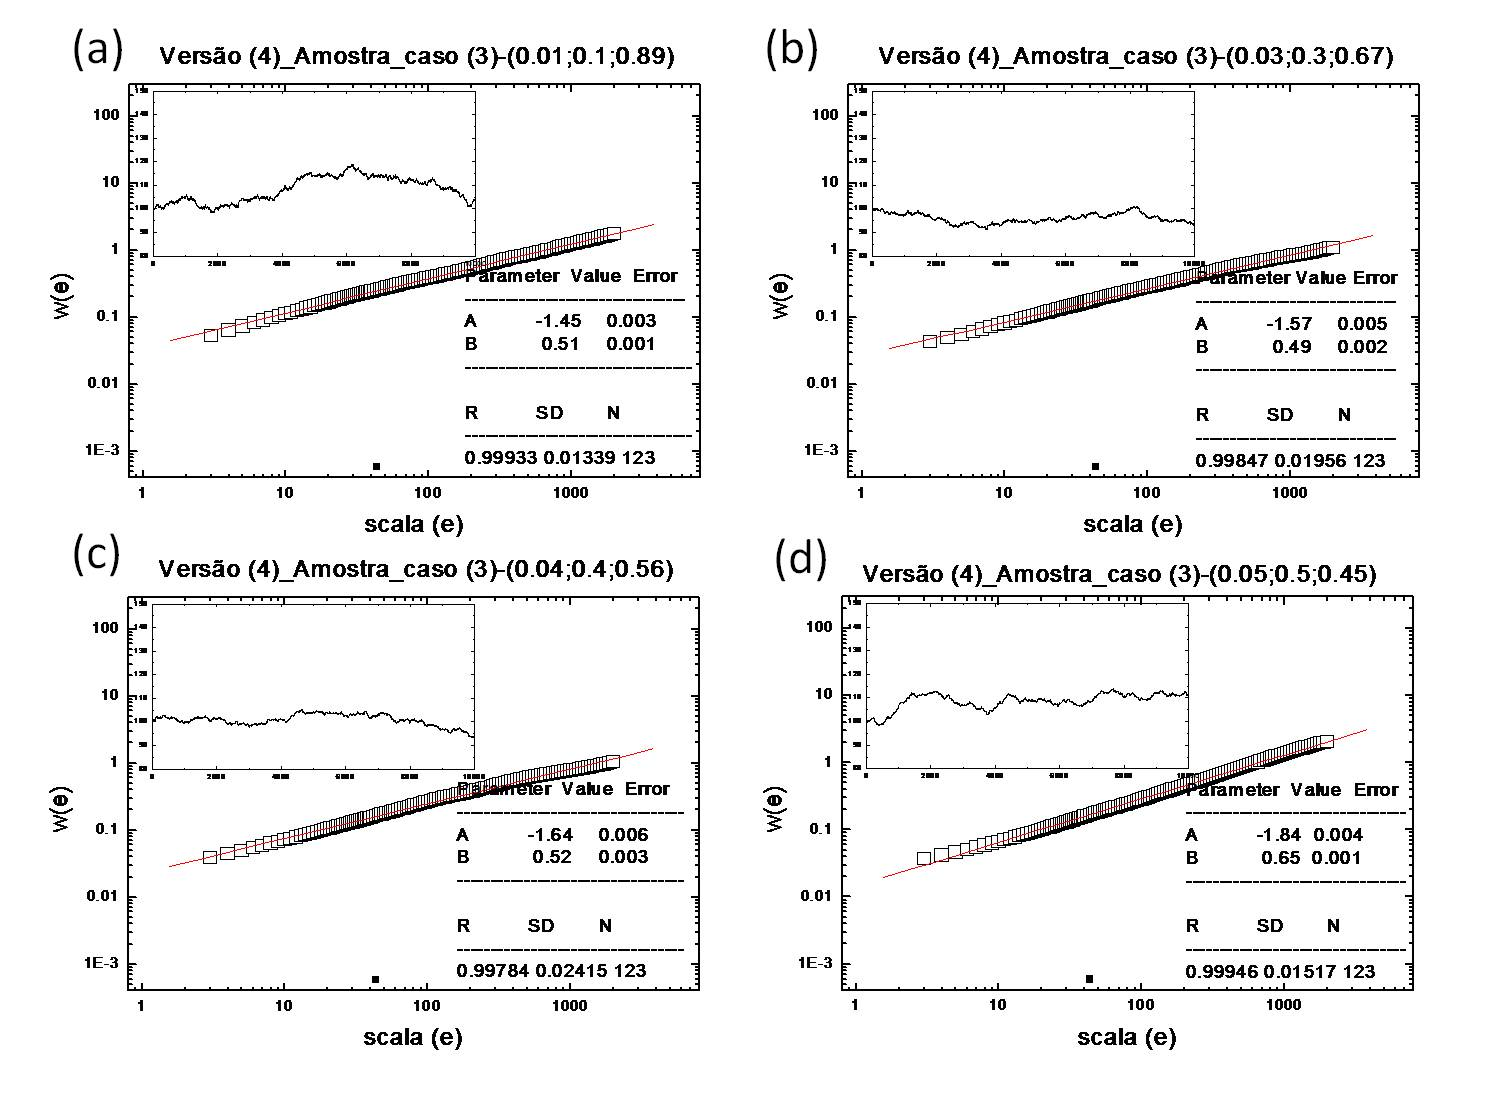
\includegraphics[width=.7\linewidth]{Figuras/31.jpg}
\caption{Cálculo do expoente de Hurst para os índices das ações de uma amostra
produzidas no caso (1) na  versão (4).  O parâmetro $B$ representa o valor de
$H$. Nos detalhes em cada painel são mostrados os gráficos do índice das ações.
Em todas as situações representamos os índices variando de 80 a 150. }
\label{fig:calculo-exp-hurst11}
\end{figure}

Em AIC.3, observamos que, aumentando o número de investidores
independentes e diminuindo o número de investidores imitadores, o mercando
também varia pouco, mantendo-se estável em todas as situações, como
exemplificado em \ref{fig:calculo-exp-hurst11}, resultado ja observado em
RIC.3 e RLC.3.

\begin{figure}[!h]
\centering
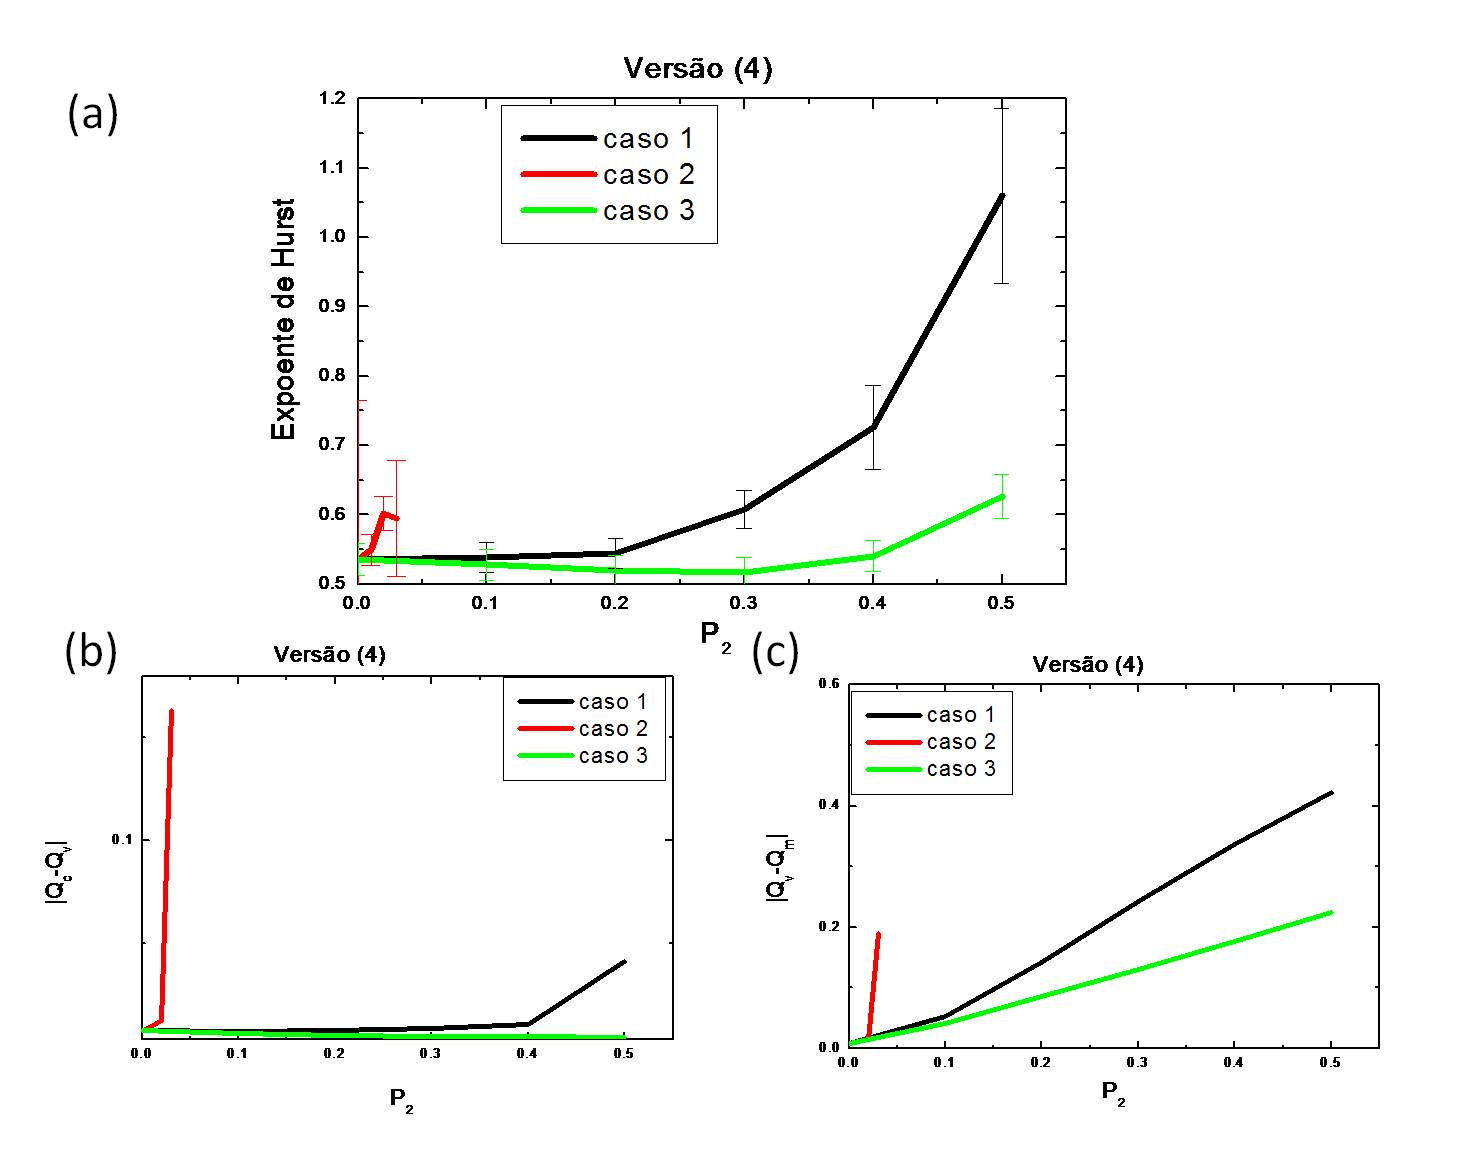
\includegraphics[width=.7\linewidth]{Figuras/32.jpg}
\caption{Na figura \ref{fig:grafico4} (a) é representado no gráfico o valor
médio das 1000 amostras do expoente de Hurst na versão (4) para cada caso em
função de $P_2$. Na figura \ref{fig:grafico4} (b) é representada a porcentagem
 da diferença entre o número de pessoas que estão
comprando ($Q_b$) e as que estão vendendo ($Q_s$) (cálculo do efeito médio de
manada para as escolhas comprar ou vender) em função de $P_2$. Na figura
\ref{fig:grafico4} (c) é representada porcentagem  da
diferença entre o número de pessoas que estão comprando ($Q_b$) e as que estão
mantendo ($Q_h$) (que é igual à diferença entre o número pessoas que estão
vendendo e as que estão mantendo) em função de $P_2$, ou seja, é calculada a
porcentagem da diminuição da escolha ``manter''.}
\label{fig:grafico4}
\end{figure}

Em AIC.1 e AIC.2, analisando a figura 5.32, observamos que o valor do expoente
de Hurst foi menor em RIC.1 e RIC.2, em que os parâmetros são o mesmos, mas
a rede é regular. Semelhante a todos os casos analisados, o efeito de``manada'',
tem também uma maior influência no valor do expoente de Hurst. 

Em AIC.1 semelhante ao RIC.1 , o aumento de $P_1$ e $P_2$ aumenta a tendência
para $H>(1/2)$, que rapidamente fica
parecida com a de países de mercados emergentes. Sendo que esse aumento é menor
comparado ao
caso da rede regular. 

Em AIC.2, por causa da quebra do mercado para $P_1>0,3$, o 
expoente de Hurst foi calculado para $P_1$ variando de 0,1 a 0,3, e o valor de
$H$ nesses casos foi menor em comparação ao RIC.2.  

Em AIC.3, semelhante a RIC.3,
observamos também a tendência de $H\sim (1/2)$, o que é esperado para um mercado
eficiente. Mesmo com o aumento de $P_2$  e com a diminuição do número de
investidores mantendo, o expoente de Hurst varia pouco.

\begin{figure}[!h]
\centering
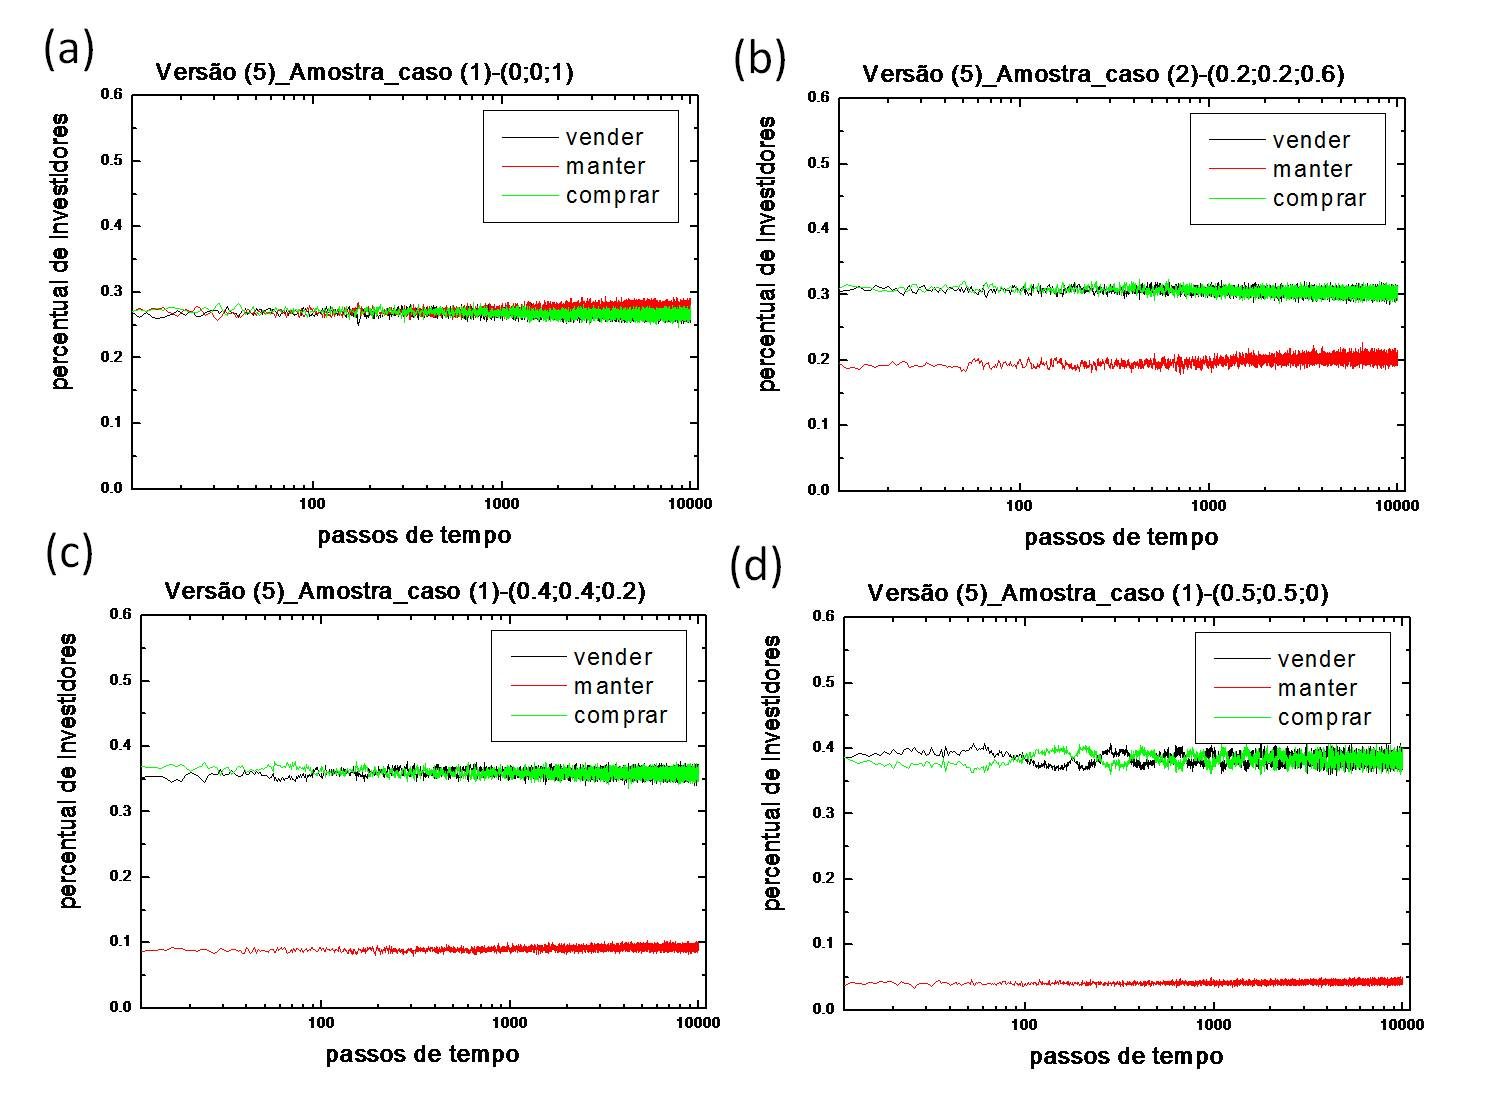
\includegraphics[width=.7\linewidth]{Figuras/33.jpg}
\caption{Evolução do comportamento dos investidores durante o tempo para caso
(1) na  versão (5) de uma amostra. Definimos a mesma escala da representação da
variação do percentual, em 0 a 0,6.  }
\label{fig:evolucao-comp-investidores9}
\end{figure}

\section{AL- Versão (5) da simulação}

Na simulação da versão (5), AL, os parâmetros são quase todos os mesmos de AI,
exceto em que a quantidade de dinheiro e ações é finita, sendo seus valores
iniciais, 10000 e 100, respectivamente. Como consequência, regras foram criadas
que estão descritas no capitulo \ref{modelo}.

\begin{figure}[!h]
\centering
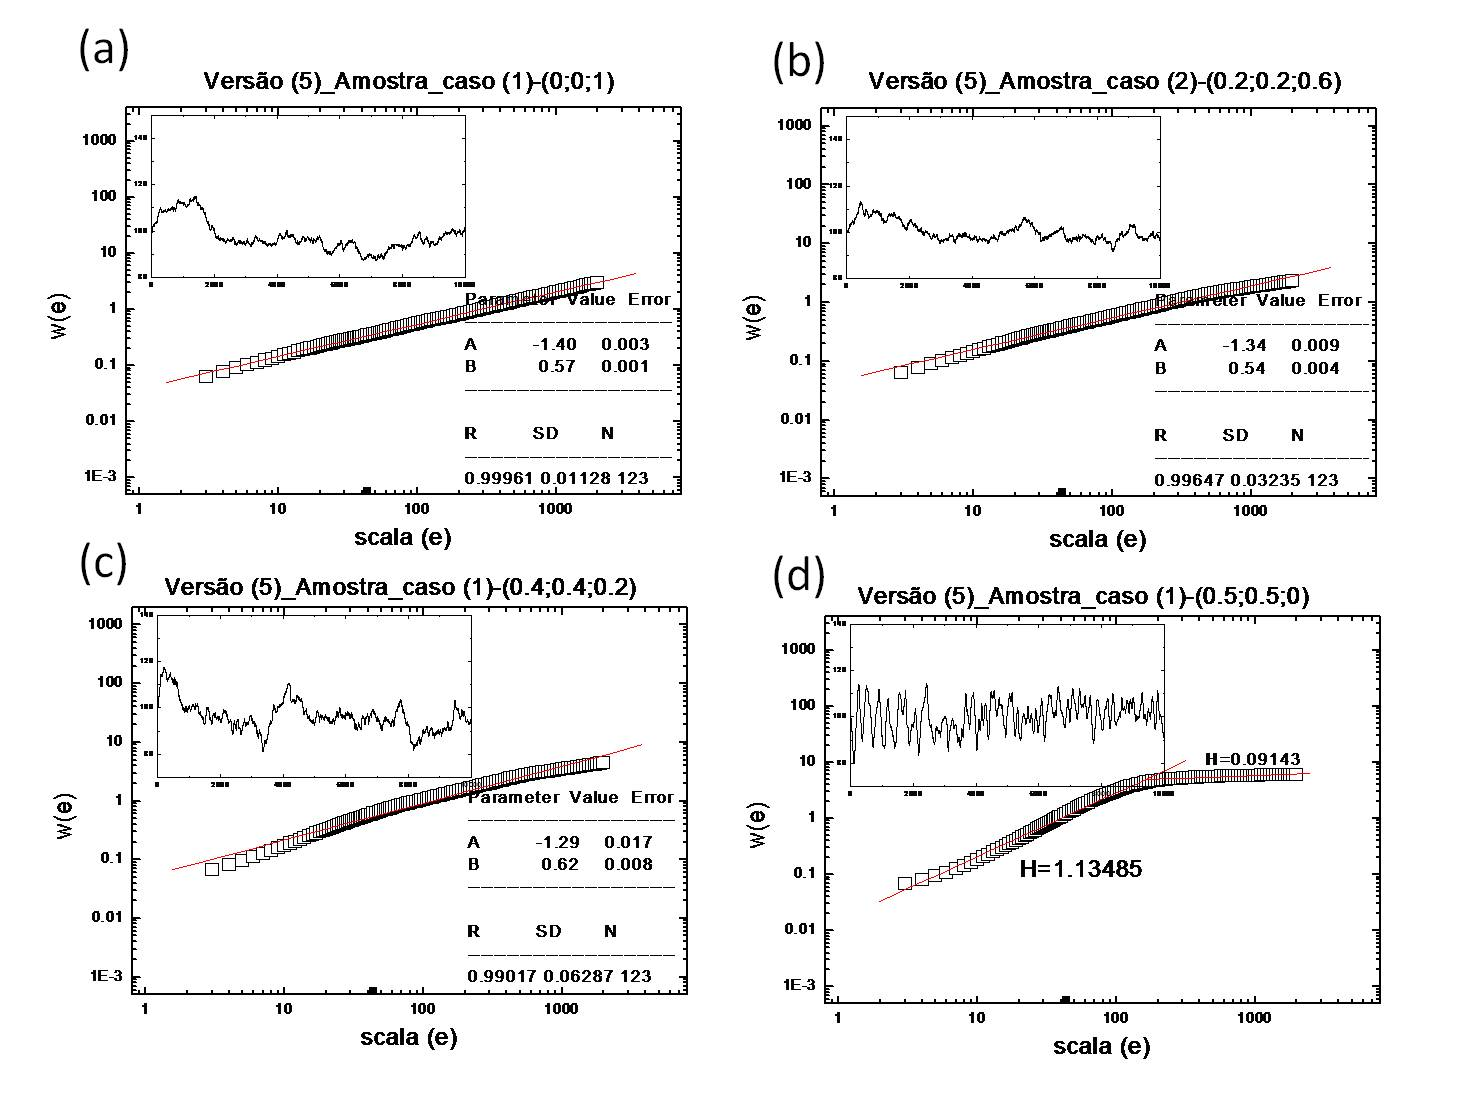
\includegraphics[width=.7\linewidth]{Figuras/34.jpg}
\caption{Em (a) e (b) Cálculo do expoente de Hurst para os índices das ações de
uma amostra produzidas no caso (1) na  versão (5).  O parâmetro $B$ representa o
valor de $H$. Nos detalhes em cada painel são mostrados os gráficos do índice
das ações. As representação dos índices esta variando de 80 a 150.  Em (c) e (d)
gráficos do índice das ações do caso (2) na versão (4). Em todos os casos o
estado inicial é aleatório com 33\% para cada opção de investimento}
\label{fig:calculo-exp-hurst12}
\end{figure}

Em ALC.1, a limitação do dinheiro influenciou
pouco nos resultados comparado ao AIC.1, observamos apenas um pequeno
aumento para a escolha manter , relação exemplificada na figura
\ref{fig:evolucao-comp-investidores9}. Em \ref{fig:evolucao-comp-investidores9}
(d), durante a simulação, em alguns instantes de tempo há um efeito de manda
para as escolha comprar, e em outros instantes esse efeito é para a escolha
comprar, significando que durante alguns intervalos de tempo os
investidores ficaram sem dinheiro ou ações; Já em comparação RLC.2, em que os
parâmetros são os mesmos, os resultados da evolução do comportamento são
diferentes,  a tendência para a escolha manter não tende a aumentar. Em relação
ao índice, nos três casos citados aqui os resultados são semelhante, exceto  em
\ref{fig:calculo-exp-hurst12} (d), em que o efeito de manda da intercalação
entre comprar e vender fica evidente.     

Em ALC.2, semelhante ao AIC.2, para $P1>0,3$ o
mercado também quebra. Nem mesmo a limitação de dinheiro faz com a quebra seja
evitada, pois isso ocorre em poucos passos de tempo. Assim, como esses
resultados são muito semelhante não colocaremos as figuras referentes as caso
ALC.2, apenas calcularemos representaremos, a seguir o valor médio
do expoente de Hurst das 1000 amostras. 

Já em ALC.3, os resultados são semelhantes as AIC.3, RIC.3, RLC.3,
por esse motivo também não colocaremos as figuras referentes a esse caso. E
também apenas representaremos, a seguir o
valor médio do expoente de Hurst das 1000 amostras. 

\begin{figure}[!h]
\centering
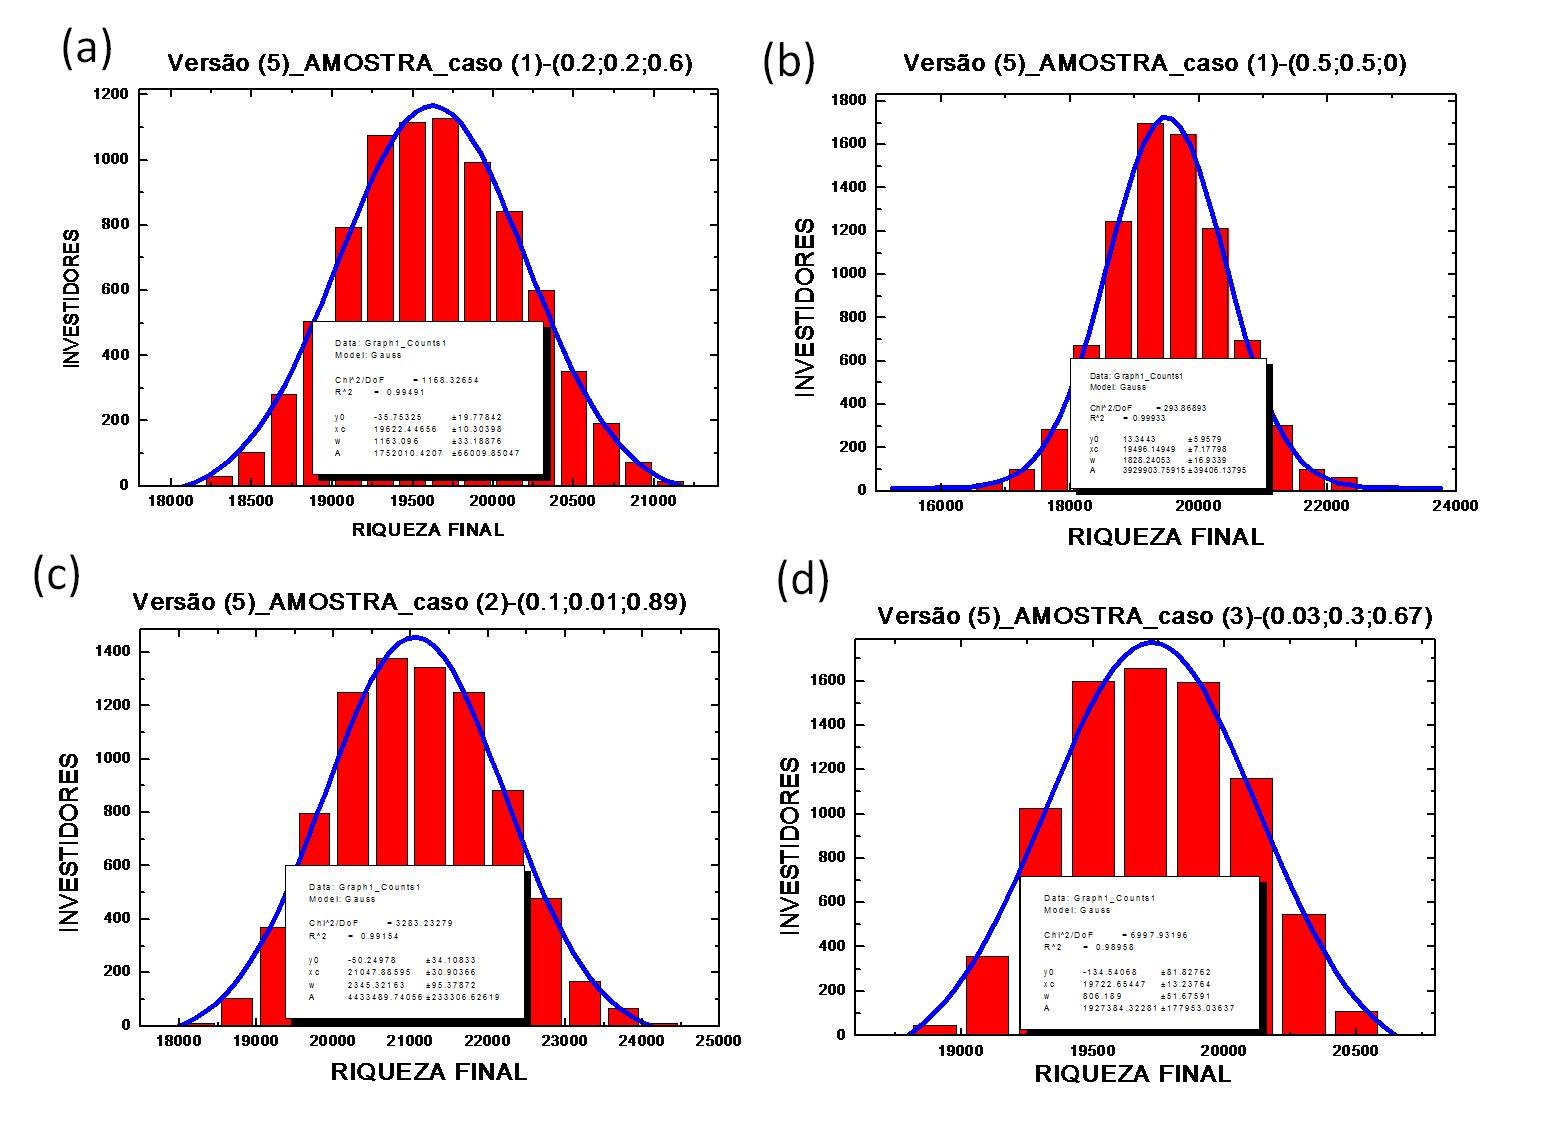
\includegraphics[width=.7\linewidth]{Figuras/35.jpg}
\caption{Histograma do dinheiro final dos investidores. (Calculo feito pela
quantidade final de ações vezes o índice atual, somado a quantidade final de
dinheiro). As figuras (a) e (b) representam o caso (1), (c)  o caso (2) e (d) o
caso (3).}
\label{fig:histograma3}
\end{figure}

Ao analisar o histograma, representado na figura \ref{fig:histograma3},
observamos  as distribuições aproximação de uma gaussiana é
mais perfeita do que as versões de redes regular.  Os resultados obtidos nessa
figura comprovam nossas conclusões acima, fica claro que há um número mínimo de
investidores falidos para todos os casos, por este motivo os investidores não
tenderam a manter, o contrário que acontece em RL, em que os
parâmetros são os mesmos, mas a rede é regular.

\begin{figure}[!h]
\centering
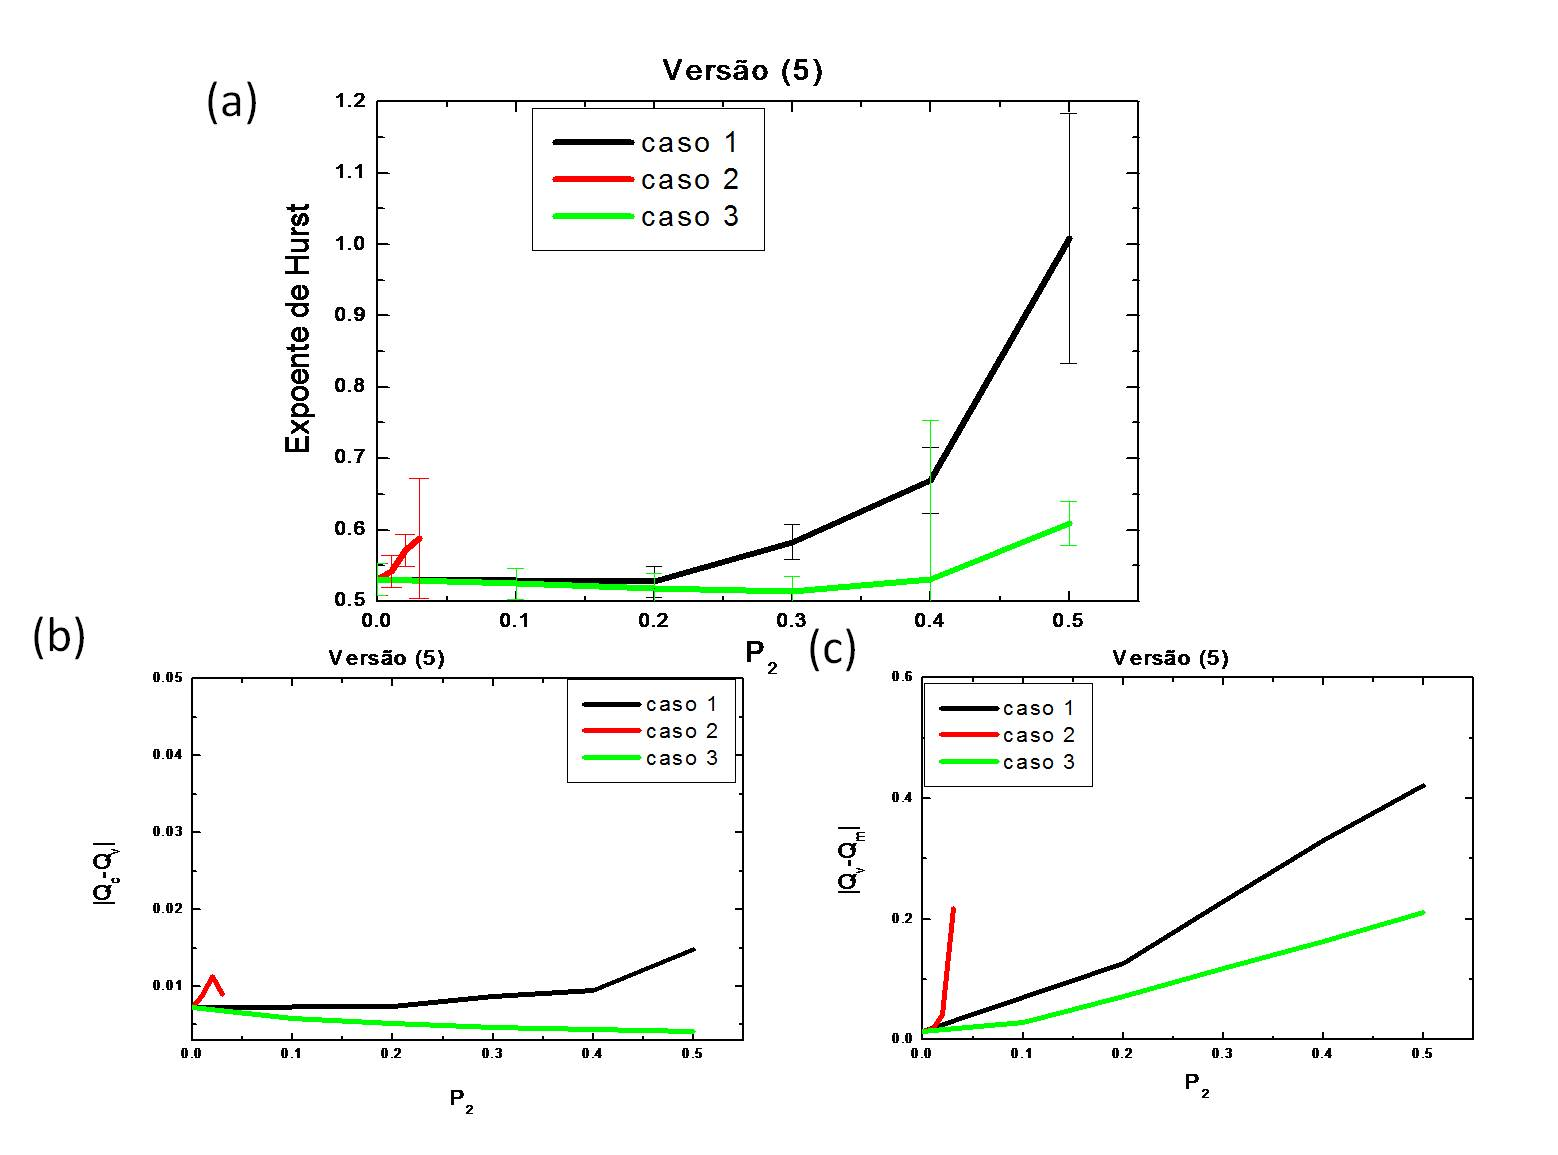
\includegraphics[width=.7\linewidth]{Figuras/36.jpg}
\caption{Na figura \ref{fig:grafico5} (a) é representado no gráfico o valor
médio das 1000 amostras do expoente de Hurst na versão (5) para cada caso em
função de $P_2$. Na figura \ref{fig:grafico5} (b) é representada a porcentagem
 da diferença entre o número de pessoas que estão
comprando ($Q_b$) e as que estão vendendo ($Q_s$) (cálculo do efeito médio de
manada para as escolhas comprar ou vender) em função de $P_2$. Na figura
\ref{fig:grafico5} (c) é representada porcentagem  da
diferença entre o número de pessoas que estão comprando ($Q_b$) e as que estão
mantendo ($Q_h$) (que é igual à diferença entre o número pessoas que estão
vendendo e as que estão mantendo) em função de $P_2$, ou seja, é calculada a
porcentagem da diminuição da escolha ``manter''.}
\label{fig:grafico5}
\end{figure}

Em ALC.1 e ALC.2, exemplificado na figura \ref{fig:grafico5},
observamos que o valor do expoente de Hurst foi menor que os mesmos casos da
em AI e RL, em que os parâmetros são quase os mesmos, exceto que em
AI o dinheiro é limitado e em RL a rede é regular. Fica claro também, o efeito
de ``manada'', tem uma maior influência no valor do expoente de Hurst. 

Em ALC.1 semelhante ao mesmo caso em AI e RL,
o aumento de $P_1$ e $P_2$ aumenta a tendência para $H>(1/2)$, que rapidamente
fica parecida com a de países de mercados emergentes. Sendo que esse aumento
comparado às
versões AI e RL foi menor. O caso C.1= (0.5;0.5;0) foi o único em que o valor de
$H$, em todas as versões manteve-se o mesmo, bem próximo de 1.  

Já em ALC.2, por causa da quebra do mercado para $P_1>0,3$, o 
expoente de Hurst foi calculado para $P_1$ variando de 0.1 a 0.3, e o valor de
$H$ nesses casos foi  também foi menor em comparação ao mesmo caso em AI e RL. 
  

Em ALC.3, semelhante ao mesmo caso em AI e RL, observamos também a tendência de
$H\sim (1/2)$, o que é esperado para um
mercado eficiente. Para $P_1$ variando de 0.1 a 0.3, o valor de $H$ foi menor em
comparação ao AIC.3.

\begin{figure}[!h]
\centering
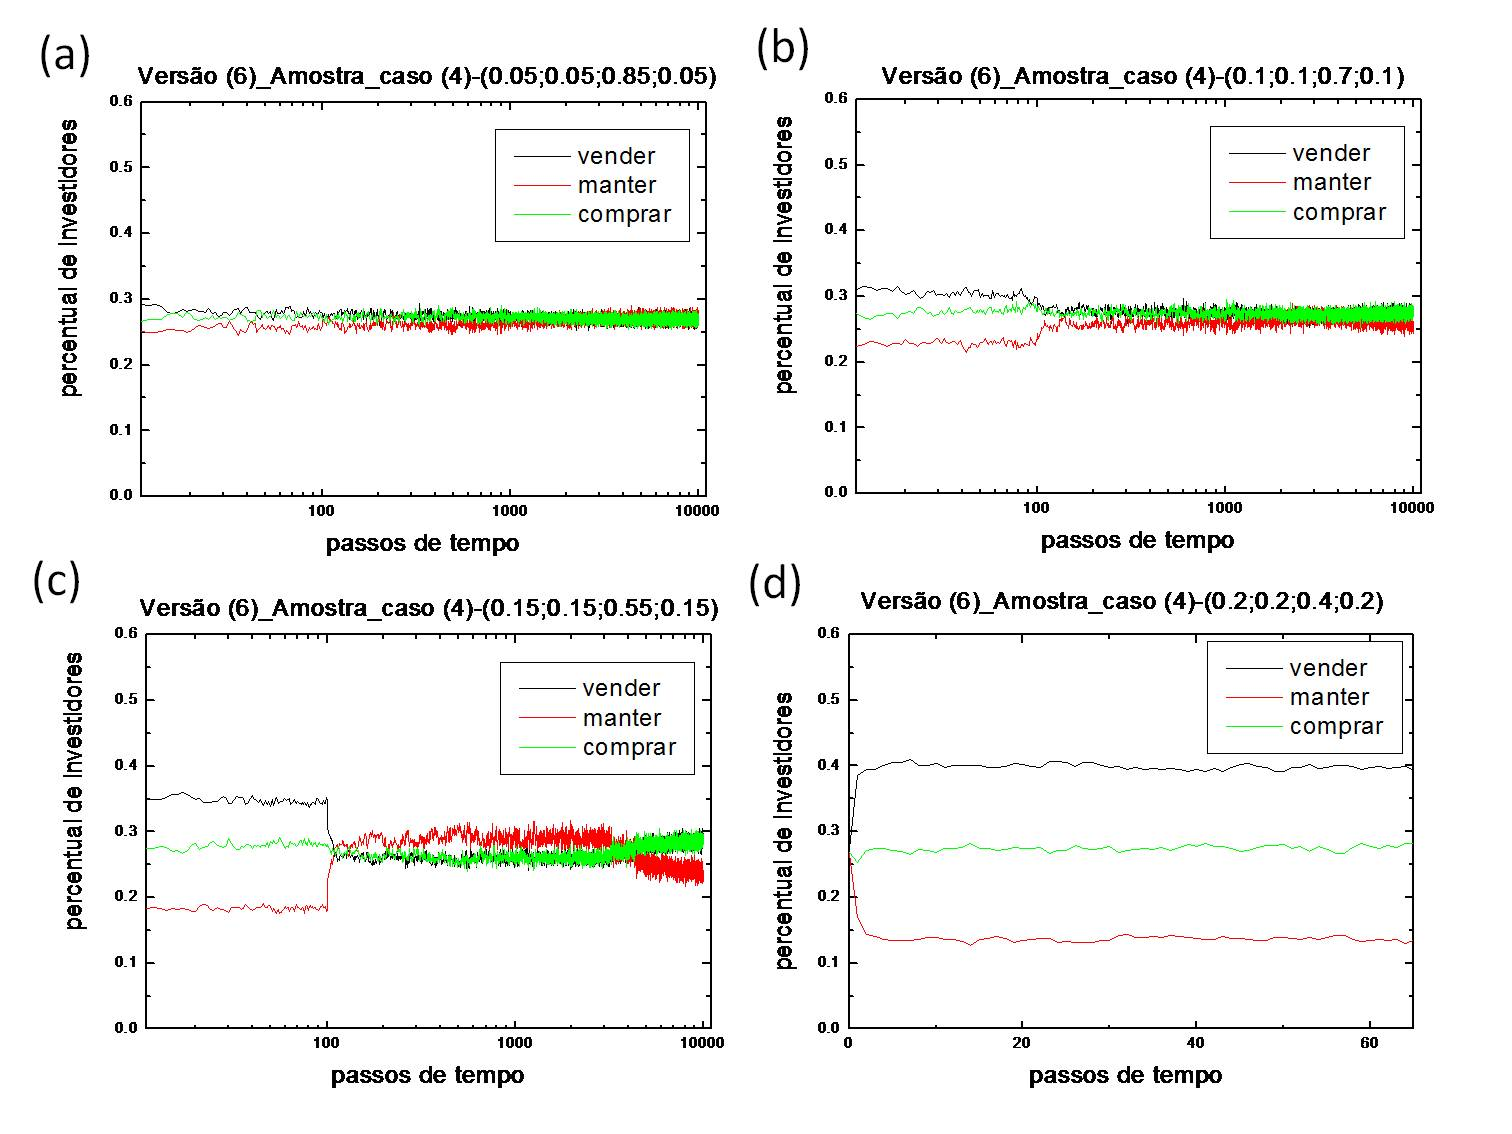
\includegraphics[width=.7\linewidth]{Figuras/37.jpg}
\caption{Evolução do comportamento dos investidores durante o tempo para caso
(4) na  versão (6) de uma amostra. Definimos a mesma escala da representação da
variação do percentual, em 0 a 0.6.  }
\label{fig:evolucao-comp-investidores10}
\end{figure}

\section{AL4- Versão (6) da simulação}

Na simulação da versão (6), AL4, semelhante à versão AL, a quantidade de
dinheiro e ações é finita, sendo seus valores iniciais, 10000 e 100,
respectivamente. Além dos três tipos de investidores, consideramos um quarto
tipo denominado ``imitador do mais rico''. Como temos quatro tipos de
investidores, os casos simulados são os C.4, C.5 e C.6.

\begin{figure}[!h]
\centering
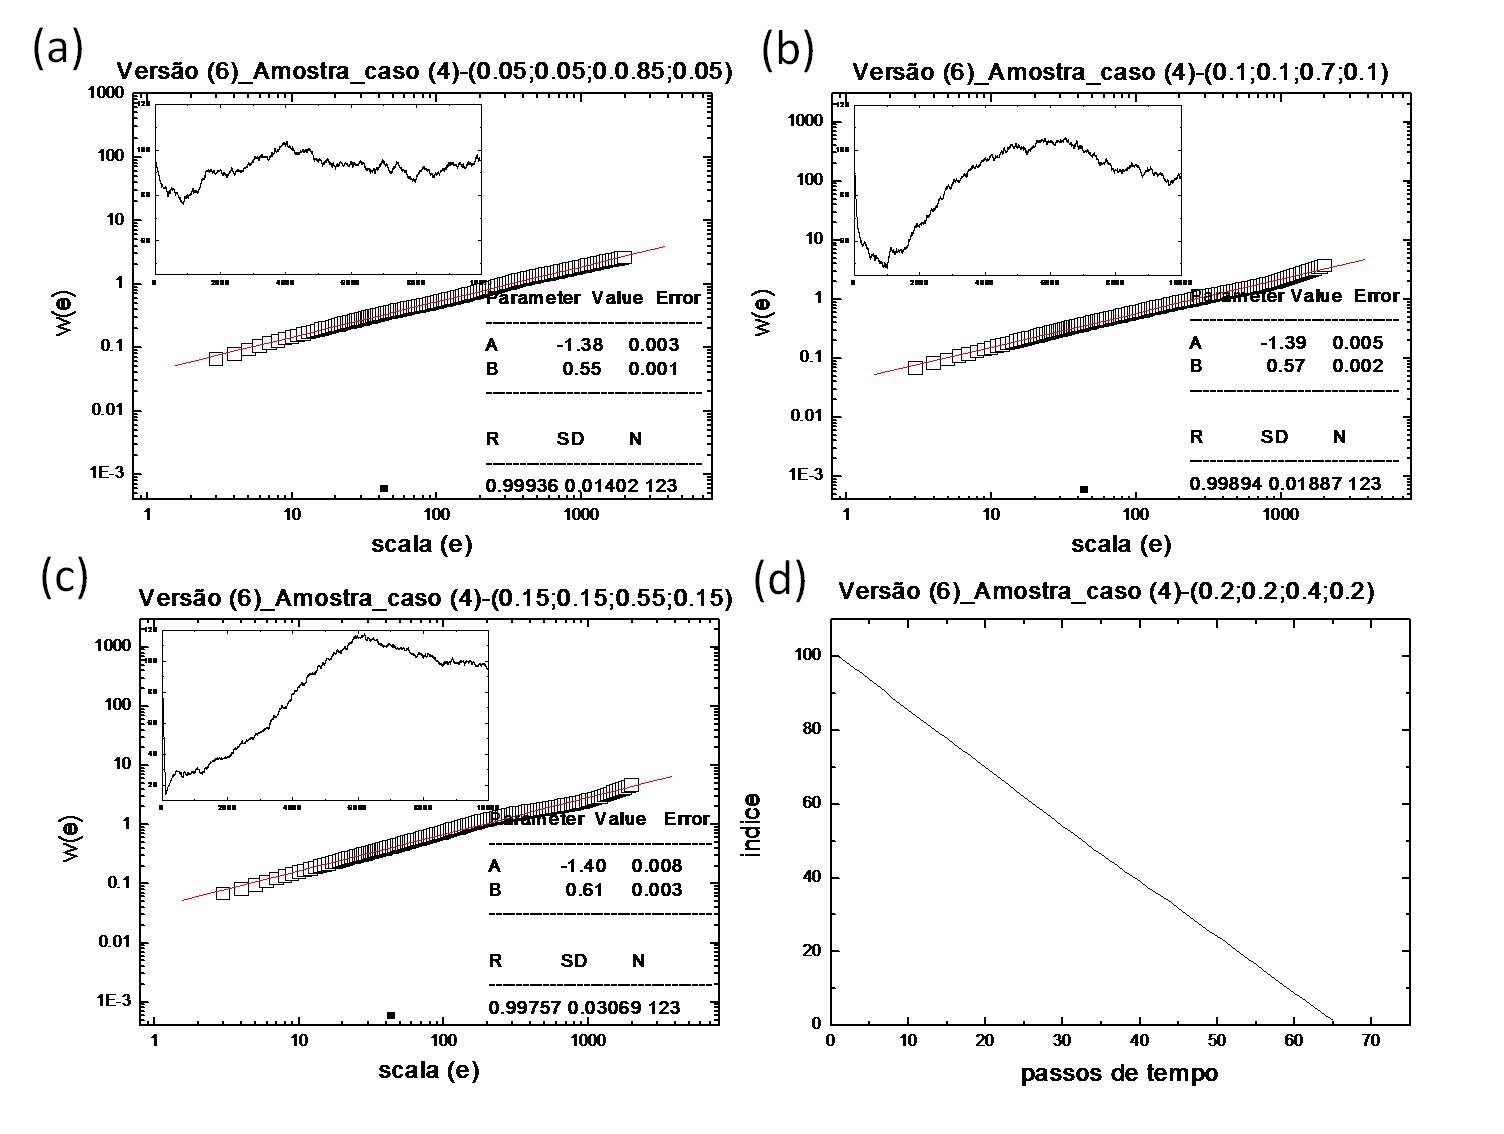
\includegraphics[width=.7\linewidth]{Figuras/38.jpg}
\caption{Em (a), (b), (c) representamos cálculo do expoente de Hurst para os
índices das ações de uma amostra produzidas no caso (4) da versão (6).  O
parâmetro $B$ representa o valor de $H$. Nos detalhes em cada painel são
mostrados os gráficos do índice das ações. As representação dos índices esta
variando de 45 a 120.  Em (d) representamos o gráfico do índice das ações do
caso (4)(0.2;0.2;0.4;0.2) da versão (6). }
\label{fig:calculo-exp-hurst13}
\end{figure}

Em AL4C.4, à medida que $P_1$ e $P_4$ aumentam, nos primeiros
passos de tempo, observamos na figura \ref{fig:evolucao-comp-investidores10} um
leve efeito de manada para a escolha vender. Depois de certo passo de tempo,
aumenta a tendência para a escolha manter, já no final da simulação essa
tendência diminui. Assim concluímos que muitos investidores, só ao final da
simulação, conseguiram recuperar suas perdas. Logo tal efeito afeta o índice,
como observado em \ref{fig:calculo-exp-hurst13} (a), (b) e (c), ao final da
simulação o mercado mantém estável. Semelhante as versões AI e AL, ocorre uma
quebra no mercado, para $(P_1+ P_4)=0,4$  o índice chega há perto de zero em
pouco tempo,
mas esse tempo é menor que nas outras versões, como exemplificado em
\ref{fig:calculo-exp-hurst13} (d). Já na simulação desse mesmo caso da
versão RL4 em que os parâmetros são os mesmos, mas a rede regular, em poucos
instantes os investidores recuperavam e voltavam perder suas ações ou dinheiro.
E na rede regular, não ocorre quebras no mercado.

\begin{figure}[!h]
\centering
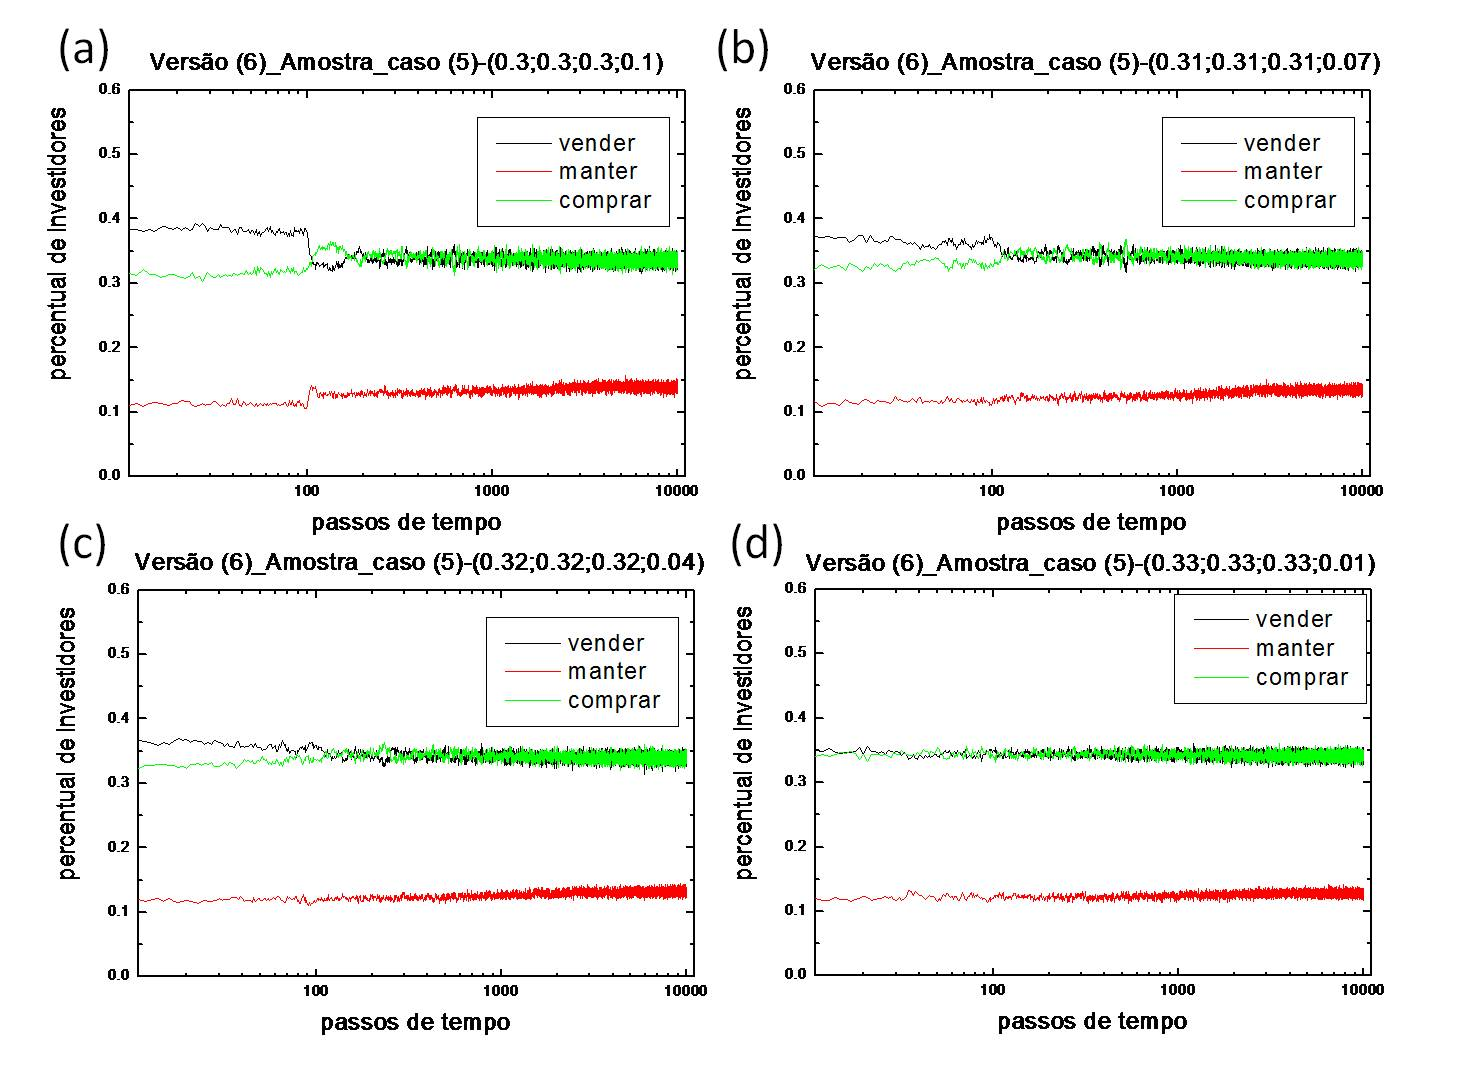
\includegraphics[width=.7\linewidth]{Figuras/39.jpg}
\caption{Evolução do comportamento dos investidores durante o tempo para caso
(5) na  versão (6) de uma amostra. Definimos a mesma escala da representação da
variação do percentual, em 0 a 0,6.  }
\label{fig:evolucao-comp-investidores11}
\end{figure}

\begin{figure}[!h]
\centering
\includegraphics[width=.7\linewidth]{Figuras/40.jpg}
\caption{Cálculo do expoente de Hurst para os índices das ações de uma amostra
produzidas no caso (5) na  versão (6).  O parâmetro B representa o valor de H.
Nos detalhes em cada painel são mostrados os gráficos do índice das ações. Em
todas as situações representamos os índices variando de 40 a 120. }
\label{fig:calculo-exp-hurst14}
\end{figure}

Em AL4C.5, os resultados são semelhante em todas as situações a
mesmo caso da versão RL4. Nos primeiros passos de tempo, observamos também um
efeito manada para a escolha vender, exemplificado na figura
\ref{fig:evolucao-comp-investidores11} principalmente, para as situações 
que possuem os maiores valores de $P_1 + P_4$. Influenciando também no aumento
do numero de pessoas que opta pela escolha manter, depois de um certo número de 
passos de tempo, como exemplificado em \ref{fig:evolucao-comp-investidores11}
(a) e (b). Significando que algumas delas ficaram sem dinheiro ou ações em
determinado tempo ou até o
final da simulação. Na figura \ref{fig:calculo-exp-hurst14}, observamos
que o índice não chega a perto de zero para $(P_1+ P_4)=0,4$ como ocorreu AL4C.4
fato se deve ao valor $P_2$ ser grande, o que minimiza o efeito de manada.

\begin{figure}[!h]
\centering
\includegraphics[width=.7\linewidth]{Figuras/41.jpg}
\caption{Evolução do comportamento dos investidores durante o tempo para caso
(6) na  versão (6) de uma amostra. Definimos a mesma escala da representação da
variação do percentual, em 0 a 0,6. }
\label{fig:evolucao-comp-investidores12}
\end{figure}

\begin{figure}[!h]
\centering
\includegraphics[width=.7\linewidth]{Figuras/42.jpg}
\caption{Cálculo do expoente de Hurst para os índices das ações de uma amostra
produzidas no caso (6) na  versão (6).  O parâmetro $B$ representa o valor de
$H$. Nos detalhes em cada painel são mostrados os gráficos do índice das ações.
Em todas as situações representamos os índices variando de 40 a 120. }
\label{fig:calculo-exp-hurst15}
\end{figure}

Em AL4C.6, o número de investidores que estão comprando e
vendendo são proporcionais, à medida que $P_2$ aumenta o número de investidores
que opta pela escolha manter diminui, durante um longo passo de tempo. Mas ao
final alguns investidores começam a opta pela escolha manter, como observado na
figura \ref{fig:evolucao-comp-investidores12}. Significando que investidores
começaram a ficar sem ações ou dinheiro. Já na figura
\ref{fig:calculo-exp-hurst15}, observamos que o mercado manteve-se estável em
todos os casos. Esses resultados
são diferentes da simulação desse mesmo caso da versão RL4 em que os parâmetros
são os mesmos, mas a rede regular.

\begin{figure}[!h]
\centering
\includegraphics[width=.7\linewidth]{Figuras/43.jpg}
\caption{Histograma do dinheiro final dos investidores. (Cálculo feito pela
quantidade final de ações vezes o índice atual, somado a quantidade final de
dinheiro). As figuras (a) e (b) representam o caso (4), (c)  o caso (5) e (d) o
caso (6).}
\label{fig:histograma4}
\end{figure}

Analisando o histograma da distribuição riqueza final dos investidores na versão
AL4, observamos que as figuras \ref{fig:calculo-exp-hurst15} no geral 
seguem uma gaussiana, mas a media que $P_4$ aumenta essa distribuição tende a
seguir uma lei da potência, como em \ref{fig:calculo-exp-hurst15} (b),(c).
Isso não acontece em AL, versão que nao temos o $P_4$. Quando há imitação do
mais rico é alta, ao final da simulçao,poucos investidores ganharão muito e
muito investidores ganharão pouco. Em todas os casos o número de falidos é zero.
Indicando que ninguém ficou sem ações e dinheiro ao final do jogo.

\begin{figure}[!h]
\centering
\includegraphics[width=.7\linewidth]{Figuras/44.jpg}
\caption{Na figura \ref{fig:grafico6} (a) é representado no gráfico o valor
médio das 1000 amostras do expoente de Hurst na versão (6) para cada caso em
função de $P_2$. Na figura \ref{fig:grafico6} (b) é representada a porcentagem
 da diferença entre o número de pessoas que estão
comprando ($Q_b$) e as que estão vendendo ($Q_s$) (cálculo do efeito médio de
manada para as escolhas comprar ou vender) em função de $P_2$. Na figura
\ref{fig:grafico6} (c) é representada porcentagem  da
diferença entre o número de pessoas que estão comprando ($Q_b$) e as que estão
mantendo ($Q_h$) (que é igual à diferença entre o número pessoas que estão
vendendo e as que estão mantendo) em função de $P_2$, ou seja, é calculada a
porcentagem da diminuição da escolha ``manter''.}
\label{fig:grafico6}
\end{figure}

Na figura 5.44, observamos também o efeito de “manada” é o que mais influência
no expoente de Hurst, como observado em \ref{fig:grafico6}. O valor máximo do
expoente de Hurst é aproximadamente 0.69, observado em \ref{fig:grafico6}(a);
menor do que o máximo, em todas as 5 versões anteriores.  


Em AL4C.4, observamos também que o aumento de $P_1$ (investidores imitadores)
juntamente com $P_4$ (imitador do mais rico) aumenta a tendência para $H>(1/2)$,
que rapidamente fica parecida com a dos mercados de países emergentes. 

Em AL4C.5, em que a porcentagem de investidores imitadores, somada à de 
imitadores do mais rico, é maior que a de investidores anti-imitadores somada
aos indiferentes; o efeito manada aumenta à medida que $P_1+P_4$ aumentam, mais
rapidamente que nos outros casos, relação o que já foi observado em RL2C.5,
fazendo, assim, que H seje maior, como em \ref{fig:grafico6}(a).   

Em AL4C.6, em que o número de anti-imitadores somado ao número de indiferentes
esta em maioria, observamos a tendência de $H\sim 0,5$, o que é esperado para um
mercado de países desenvolvidos. Mesmo com o aumento de $P_2$, e com a
diminuição do número de investidores que estão no estado manter, o expoente de
Hurst também varia pouco.

\begin{figure}[!h]
\centering
\includegraphics[width=.7\linewidth]{Figuras/tabela1.jpg}
\caption{Média do Expoente de Hurst - Caso (1)}
\label{fig:tabela1}
\end{figure}

\begin{figure}[!h]
\centering
\includegraphics[width=.7\linewidth]{Figuras/tabela2.jpg}
\caption{Média do Expoente de Hurst - Caso (2)}
\label{fig:tabela2}
\end{figure}

\begin{figure}[!h]
\centering
\includegraphics[width=.7\linewidth]{Figuras/tabela3.jpg}
\caption{Média do Expoente de Hurst - Caso (3)}
\label{fig:tabela3}
\end{figure}

\begin{figure}[!h]
\centering
\includegraphics[width=.6\linewidth]{Figuras/tabela4.jpg}
\caption{Média do Expoente de Hurst - Caso (4)}
\label{fig:tabela4}
\end{figure}

\begin{figure}[!h]
\centering
\includegraphics[width=.6\linewidth]{Figuras/tabela5.jpg}
\caption{Média do Expoente de Hurst - Caso (5)}
\label{fig:tabela5}
\end{figure}

\begin{figure}[!h]
\centering
\includegraphics[width=.6\linewidth]{Figuras/tabela6.jpg}
\caption{Média do Expoente de Hurst - Caso (6)}
\label{fig:tabela6}
\end{figure}

Essa versão é que mais possui criterios semelhantes aos mercados
reais.Comparando o valor AL4, nas tabelas acima, com outras versões analisadas,
observamos que os valores do
expoente de Hurst estão mais próximos dos valores esperados para o mercado
real.  

\chapter{Conclusão e Perspectivas }\label{conclusao-perspectivas}

Nesta dissertação, propusemos um modelo de mercado financeiro artificial baseado
em agentes, por um modelo de autômato celular, com dois tipos diferentes de
redes, a regular com oito vizinhos e a aleatória referente à teoria de redes
complexas. Consideramos quatro tipos diferentes de agentes o imitador, o
anti-imitador, o indiferente e o imitador do mais rico. 

Simulamos seis versões diferentes. Nas versões RI, RL e RL4 baseamos nosso
modelo na rede regular, sendo que, em RI, consideramos apenas três tipos de
investidores e a quantidade de dinheiro e ações iniciais era ilimitada; em RL,
essa quantidade era limitada. Na RL4, além dos parâmetros da RL, acrescentamos
um quarto tipo de investidor, o imitador do rico.  Em AI , AL e AL4 nosso modelo
foi baseado na teoria das redes aleatórias, o que torna nosso mercado mais real,
pois o número de conhecidos de cada investidor é variado, existindo pessoas com
apenas um ou dois amigos e outras com vários amigos que investem no mercado. Nos
modelos baseados em redes aleatórias, a cada versão, usamos os mesmos parâmetros
dos modelos baseados em redes regulares. Assim, a cada versão simulada, o
mercado tornava-se cada vez mais real. Em cada versão, analisamos o índice do
mercado obtido, calculando o expoente de Hurst e a distribuição final da riqueza
de cada investidor, com o objetivo de validar nosso modelo e comparar os
resultados com o mercado real.  

O expoente de Hurst é proposto na literatura para classificar os índices de
mercado dos países e ser usado como uma medida da eficiência do mercado. Se
persistência de longo alcance está presente nos retornos dos ativos financeiros,
a hipótese o mercado eficiente não é válida. Segundo Cajueiro
\cite{CaTa04,CaTa08}, o valor do expoente de Hurst nos mercados de ações em
mercados desenvolvidos – onde é válida a hipótese de mercado eficiente – deve
estar próximo de $H=0,5$. Em mercados emergentes, seu valor é maior que 0.5. Em
nosso mercado artificial, o valor do expoente de Hurst aproxima-se desses
valores esperados, principalmente nas versões, em que a quantidade de dinheiro e
ações é limitada (semelhante à vida real). Com isso, o modelo foi capaz de
reproduzir a complexidade do mercado em grau comparável à realidade e, portanto,
é condizente com os mercados da vida real.                    



Em todos os casos, evidenciou-se que o aumento do percentual de investidores
imitadores influencia no aumento das flutuações e do efeito de manada. E esses
aumentos influenciam diretamente no expoente de Hurst. Na rede regular, o
aumento do número desses investidores faz com que o número de falidos também
aumente. Já na rede aleatória, o índice do mercado quebra, em poucos passos de
tempo, nos casos com percentual alto de imitadores. Tal fato se explica por ser
uma rede de alto alcance onde  esse efeito se dissemina mais rapidamente.   

No caso do imitador do mais rico, que é também um tipo de imitação, observamos
que sua influencia é alta, produz resultados interessantes. Além dos efeitos
semelhantes ao “imitador”, verificamos que, na rede regular, quando seu valor é
pequeno, os investidores perdem e recuperam suas ações e seu dinheiro em poucos
instantes de tempo. Em redes aleatórias, o aumento do número de investidores que
usam essa estratégia faz com que a distribuição final do dinheiro tenda a seguir
uma lei da potência. 

Já o aumento do número de investidores anti-imitadores faz com que o mercado
flutue pouco; o efeito de manada e o valor do expoente de Hurst diminuem,
tornando o índice semelhante aos do mercado eficiente.  Na rede regular, o
número de investidores falidos é menor. Na rede aleatória, a distribuição final
da riqueza tende a seguir uma gaussiana.                              
Os investidores indiferentes produzem efeitos semelhantes aos anti-imitadores; a
união dos dois em grandes percentuais faz com que o mercado se torne o mais
eficiente possível.  

O comportamento tipo imitador e principalmente do imitador do mais rico no
modelo pode ser relacionado aos investidores racionais da hipótese do mercado
eficiente, aqueles que seguem a tendência. Já os investidores anti-imitadores e
os indiferentes são considerados os “irracionais” das finanças comportamentais.
Com os resultados, evidenciou-se que a estabilidade do mercado é afetada pela
preferência de investimento. Quando o comportamento do investidor é afetado
apenas pelo comportamento de outros investidores, como explicado acima,
espera-se que enormes flutuações ocorram no mercado – efeito de “manada”. Quando
o número de investidores imitadores e imitadores do mais rico é alto, o expoente
de Hurst é bem maior  que 0,5; desse modo, a hipótese  do mercado eficiente não
é válida. Em todos os casos simulados, verificamos que quanto maior o número de
investidores indiferentes e menor o número de investidores imitadores e
imitadores do mais rico, mais próximo de 0,5 está o H, que é o esperado para os
mercados desenvolvidos (mercados eficientes). Assim, se o comportamento dos
investidores é totalmente independente, espera-se uma maior estabilidade do
mercado de ações.  Ou seja, a maior diversidade de ponto de vista dos
investidores e a menor imitação promoverão melhor desenvolvimento do mercado.
Observamos, também, que resultado final é imprevisível a partir do estado
inicial, o que revela um grau de complexidade do modelo para reproduzir o
mercado de ações. De acordo com esses resultados, conclui-se que a modelagem por
meio de autômatos celulares é capaz de reproduzir com verossimilhança o
comportamento do mercado de ações.
 
Apesar dessa verossimilhança, sabemos que nosso modelo ainda possui limitações
comparadas aos mercados reais como: ignorar a existência de outros tipos de
estratégicas dos investidores, por exemplo, a análise gráfica; a utilização de
apenas um ativo financeiro sem a possibilidade de compor uma carteira; a mudança
de estratégia, durante a simulação; a implementação de redes de mundo pequeno; a
variação da quantidade de dinheiro e de ações iniciais. Assim, como trabalho
futuro, podem ser implementadas melhorias visando aprimorar e sanar essas
limitações. Contudo voltamos a ressaltar que nosso modelo é valido e
possibilitou várias conclusões interessantes.   


\input{dissertacao.bbl}

%\nocite{*}
%\bibliography{dissertacao}


\end{document}


